\chapter{信号优化}\label{chap:signal_optimization}
在初步筛选之后,为了进一步加强信号显著性,利用动力学性质进行信号优化是有必要的。因为每个信号质量点的动力学性质差别
较大,所以,每个质量点都会进行信号优化过程,而后通过各自
动力学选择条件之后的区域才作为每个质量点的最终信号区。

\section{优化策略}
MVA方法用于确定不同运动学变量的分离能力,并考虑所有变量之间的相关性。最终,前五个运动学变量用于形成优化选择,分别是$M(\ell\ell)$,$\Delta R_{min}(\ell_{2}, j)$,$\Delta R_{min}(\ell_{1}, j)$ ,$ M_{\ell_{1} jj}$和$M(all)$,它们具有很强的分离能力,而且相互之间的相关性很低(图~\ref{fig:correlation_check})。通常,$M(\ell\ell)$和$ M_{\ell_{1} jj} $对低质量点敏感,而其余对高质量和非共振信号敏感。
基于这些知识,$\Delta R_{min}(\ell_{1}, j)$,$M(\ell\ell)$,$ M_{\ell_{1}jj}$和$M(all)$用于在低质量搜索中形成优化削减,而$\Delta R_{min}(\ell_{2}, j)$,$\Delta R_{min}(\ell_{1}, j)$,$M(\ell\ell)$和$M_{\ell_{1}jj}$用于高质量搜索中。它们的相应分布分别见图~\ref{fig:SigOpt_low_kine}和图~\ref{fig:SigOpt_high_kine}。\\
TMVA包(CutsSA选项)~\cite{Hocker:2007ht}用于实现最佳筛选。所有背景:promptSS,$V\gamma$,QmisID和fakes都包含在训练中。
为了减少对变量筛选顺序的依赖,每次仅训练2个变量。
在每个信号效率工作点(WP),在测试样本中对每个事例应用对应的选择条件,
并计算显著性($S/\sqrt{B}$)。随后,选择具有最高信号显著性的WP,对应该WP的2个变量筛选值即为最佳选择,
最后再对剩下两个变量重复以上步骤。图~\ref{fig:nonres:SigOpt_mumu}展示SM希格斯粒子对搜寻中$\mu\mu$分析道的效率,各个运动学
变量的选择上下限以及显著性随信号效率WP的分布。
对剩余的分析道或者其他质量点重复此操作,即可得到所有质量点的分析道的最佳优化选择条件。 \\
最终考虑从低到高(和非共振)质量点筛选值的单调性,一定的选择调整被执行。最终的选择总结在表~\ref{optimization_cuts_lowmass}和表~\ref {optimization_cuts_highmass}中,分别对应于低质量搜索和高质量搜索。

\begin{figure}[h]
\begin{center}
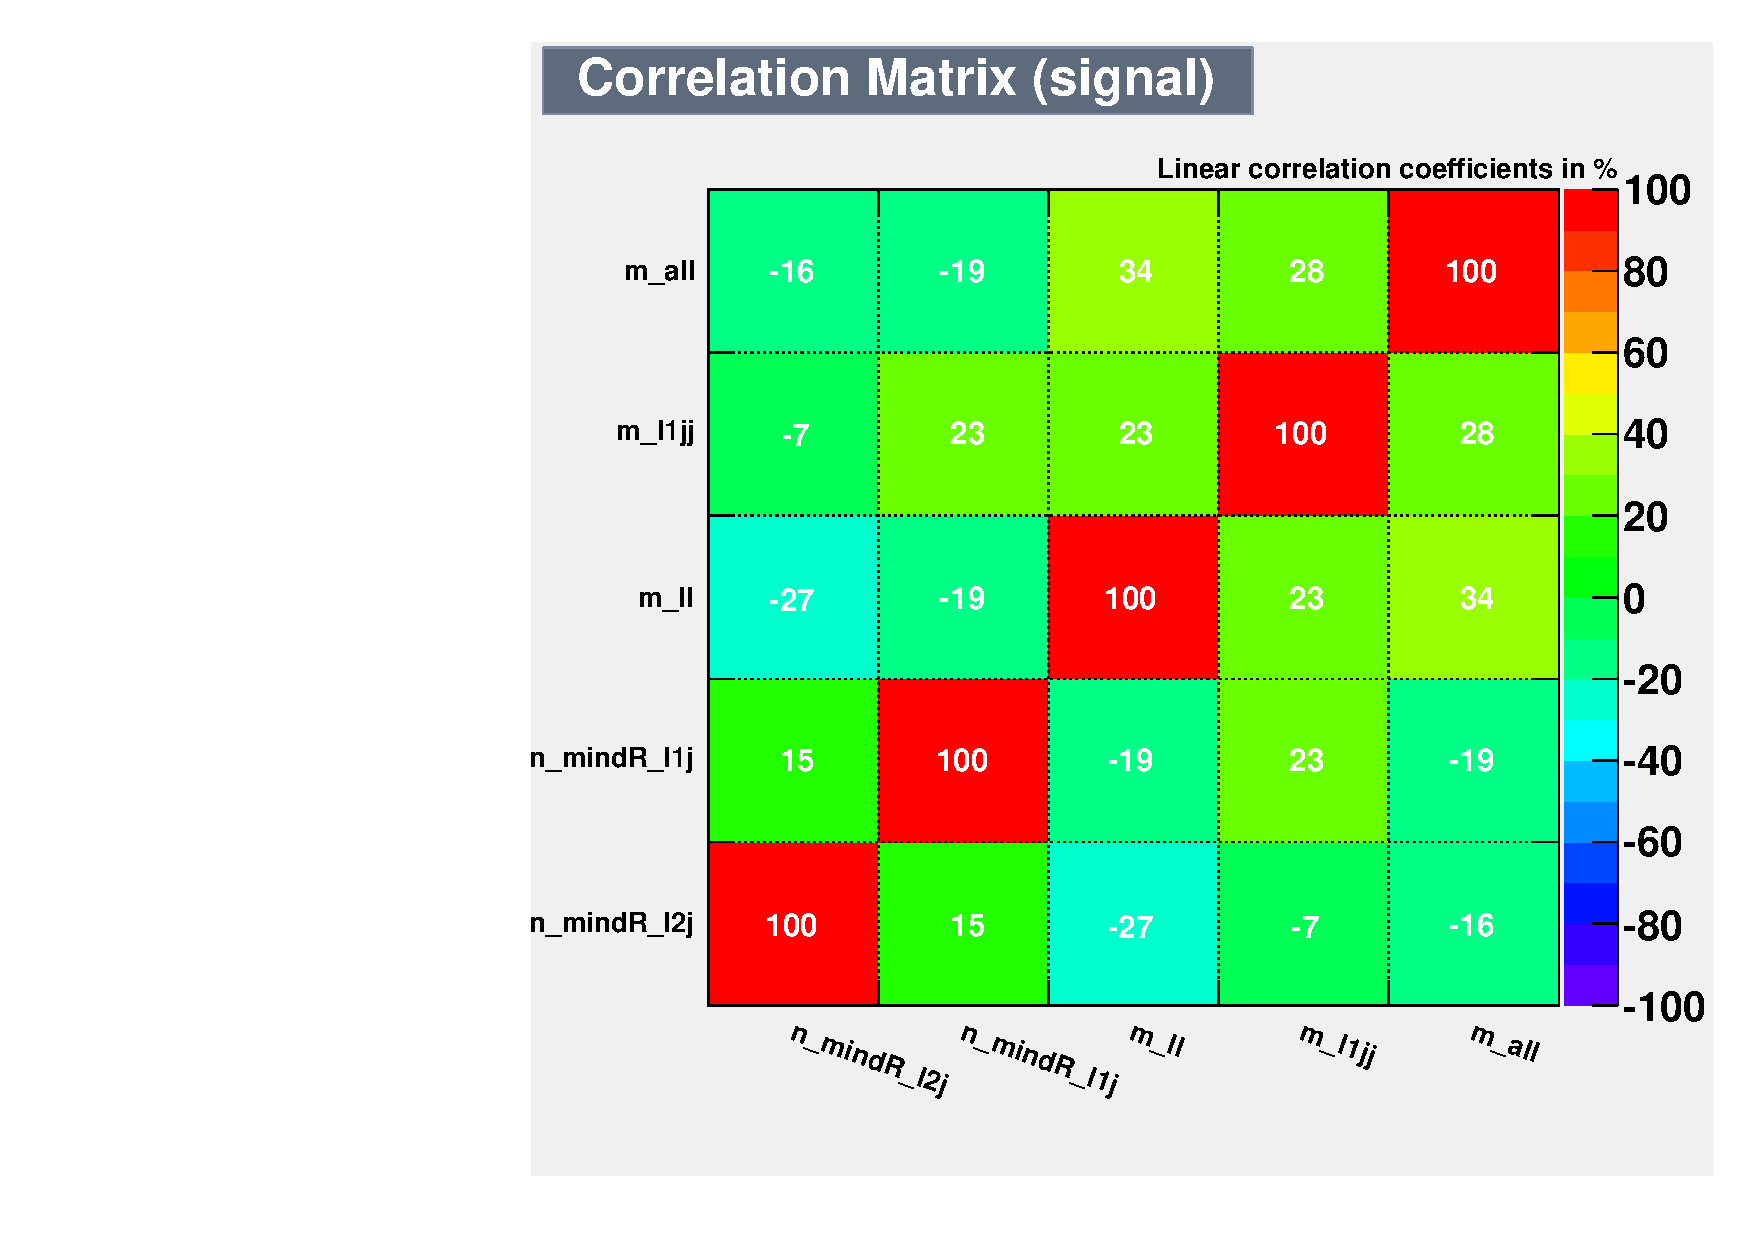
\includegraphics[width = 0.4\textwidth,angle=-90]{fig/SigOpt/correlation_signal.pdf}
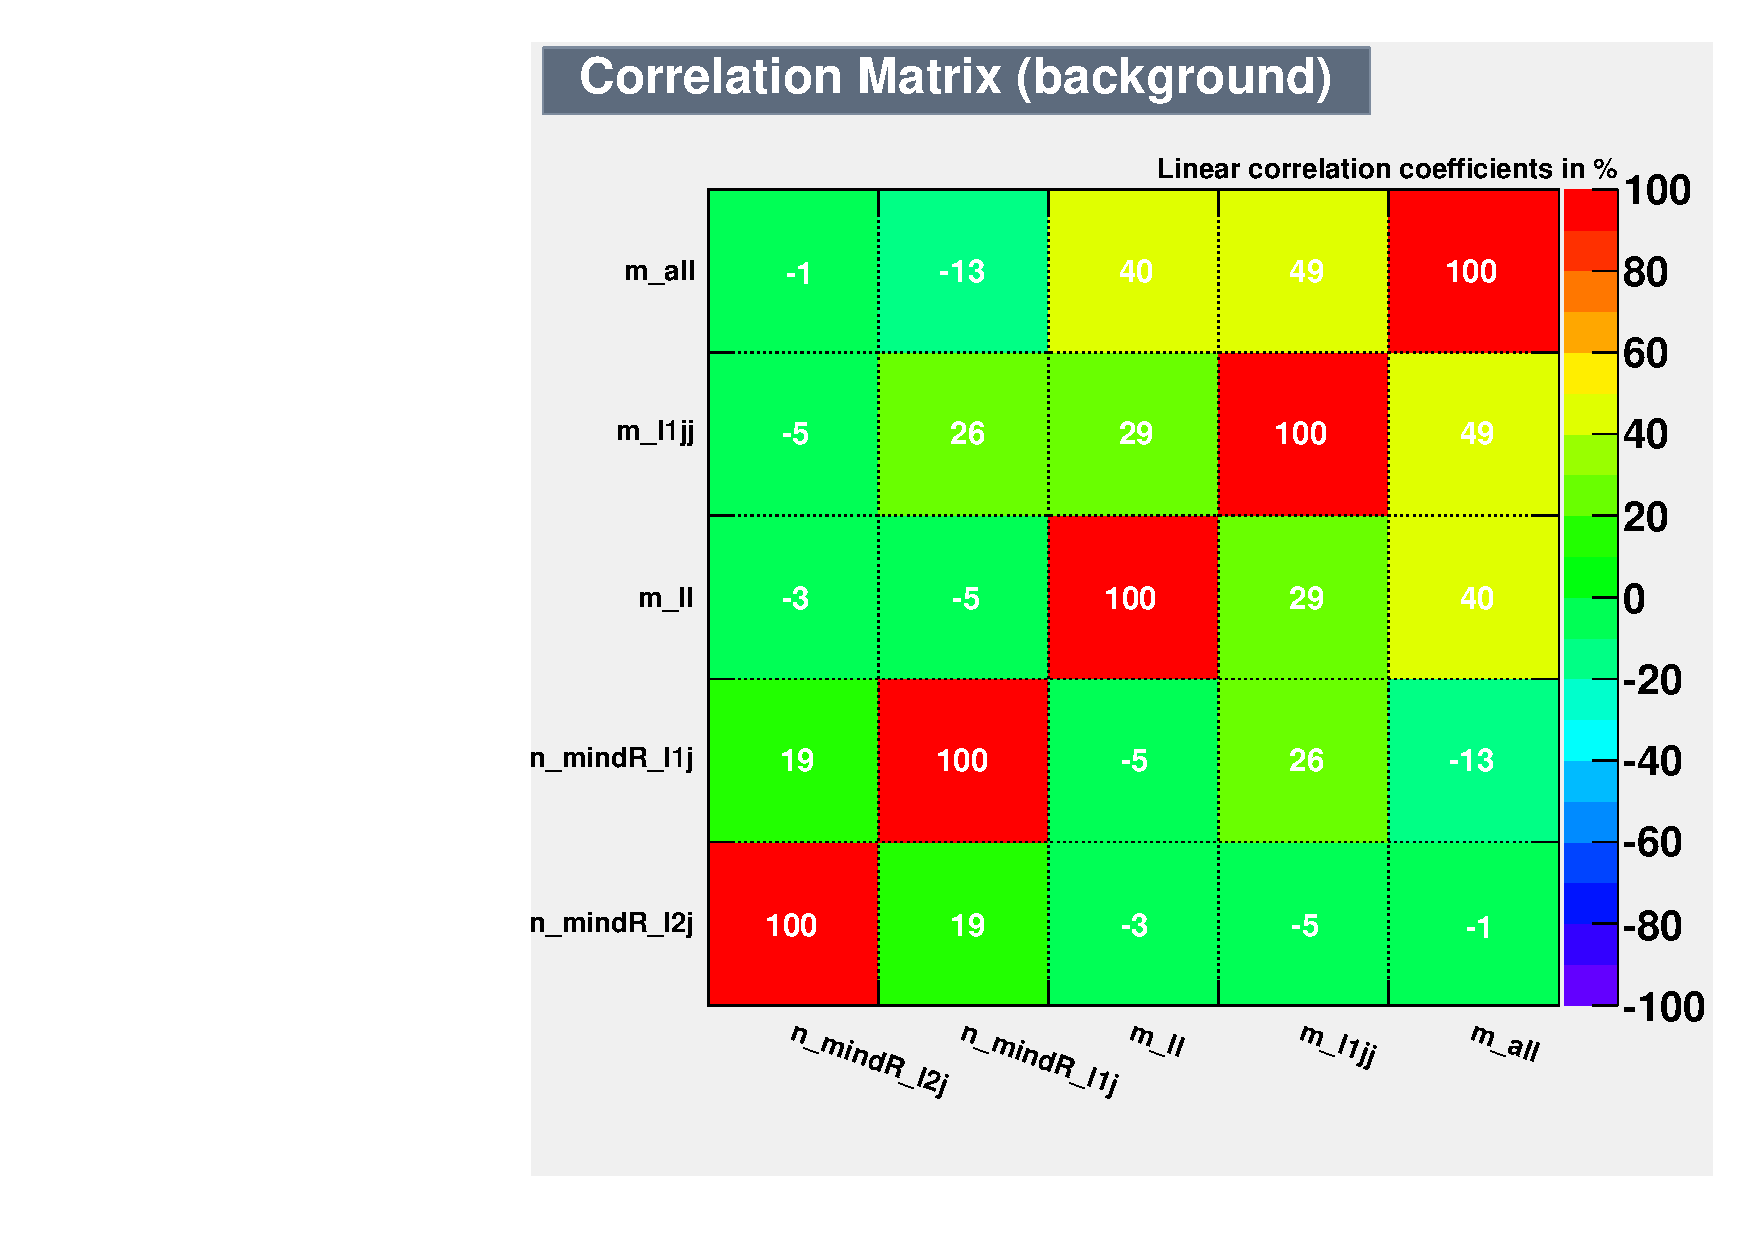
\includegraphics[width = 0.4\textwidth,angle=-90]{fig/SigOpt/correlation_bkg.pdf}
\caption{Correlation check of input training variables.} \label{fig:correlation_check}
\end{center}
\end{figure}

\begin{figure}[h]
\begin{minipage}[t]{0.33\linewidth}
 \centering
 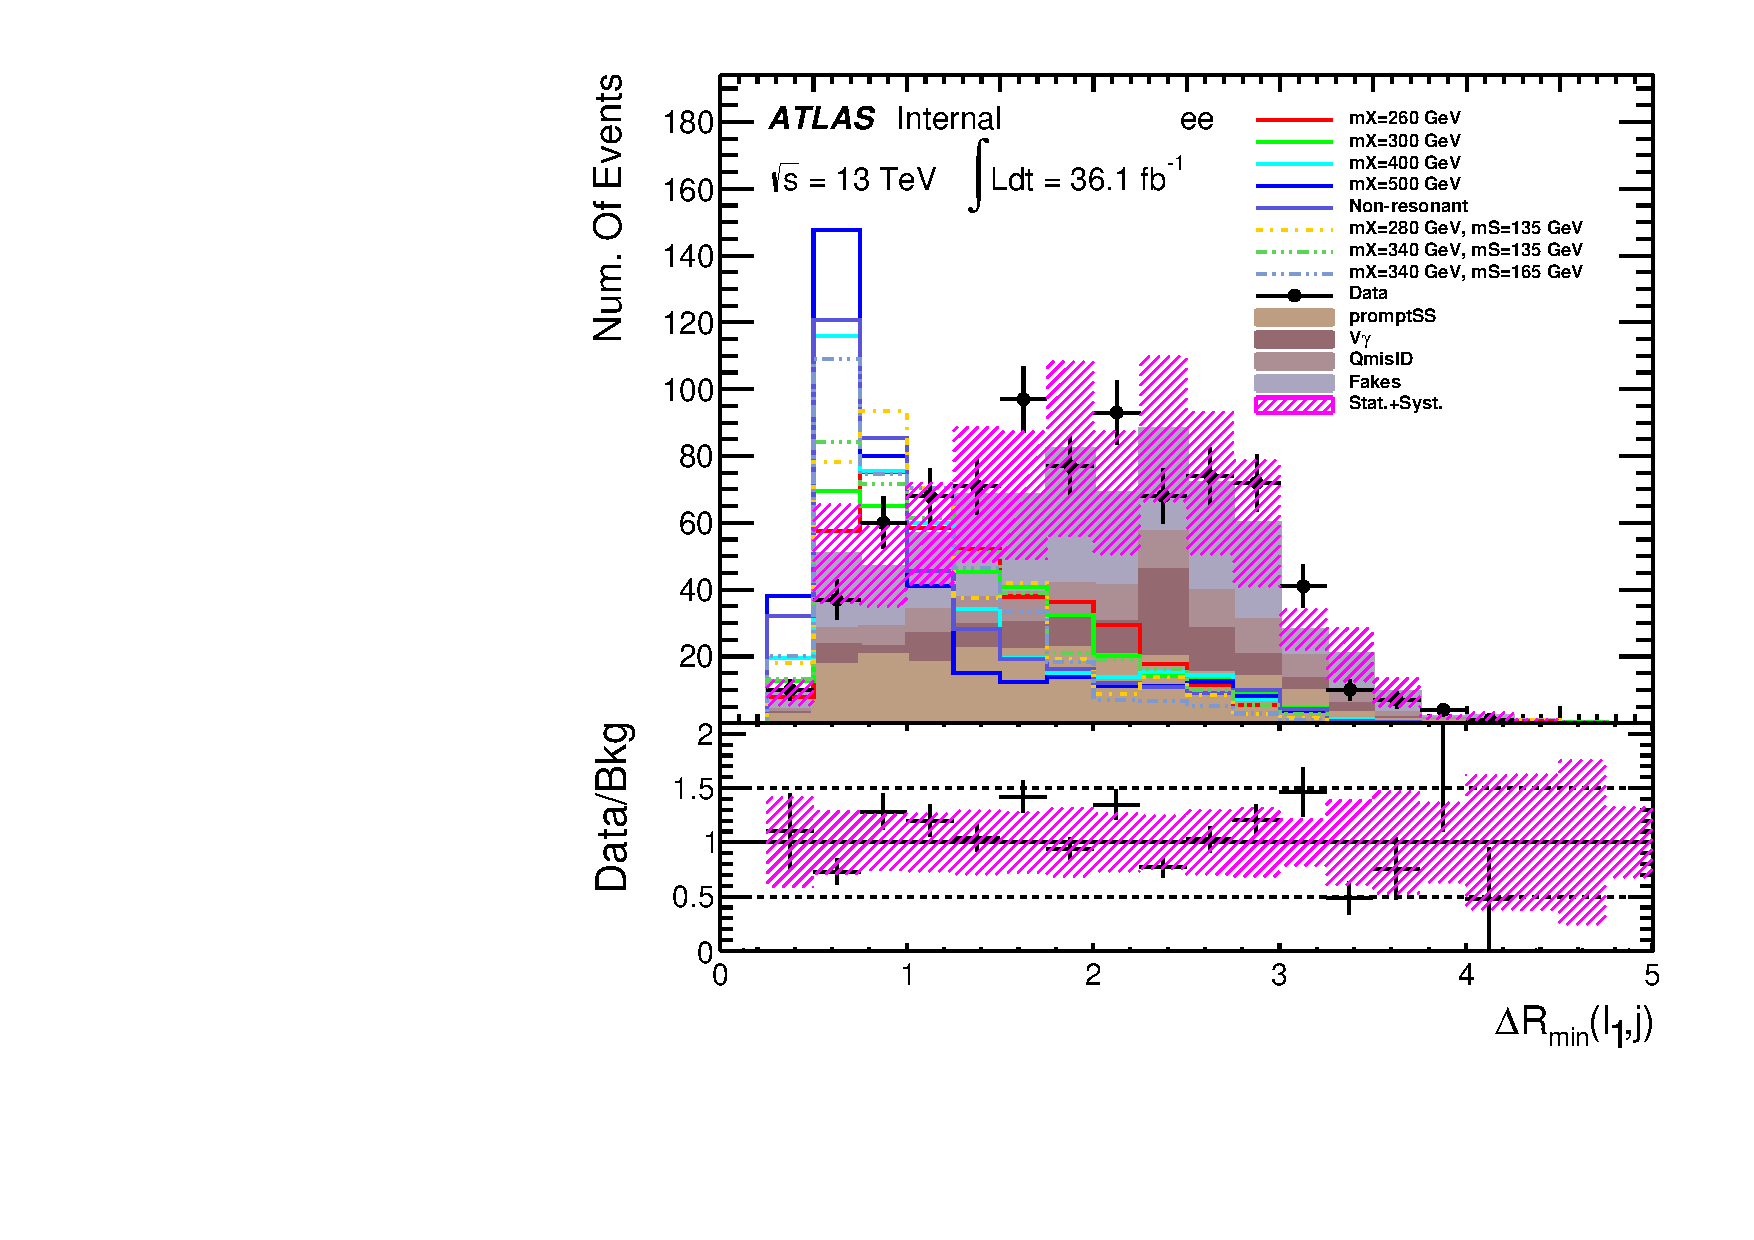
\includegraphics[width=1.0\textwidth]{fig/dataMC_low_Njet_CR/mindR_l1j_ee.pdf}\label{fig:dataMC_low_Njet_CR:mindRl1j_ee.pdf}
 \end{minipage}
 \begin{minipage}[t]{0.33\linewidth}
 \centering
 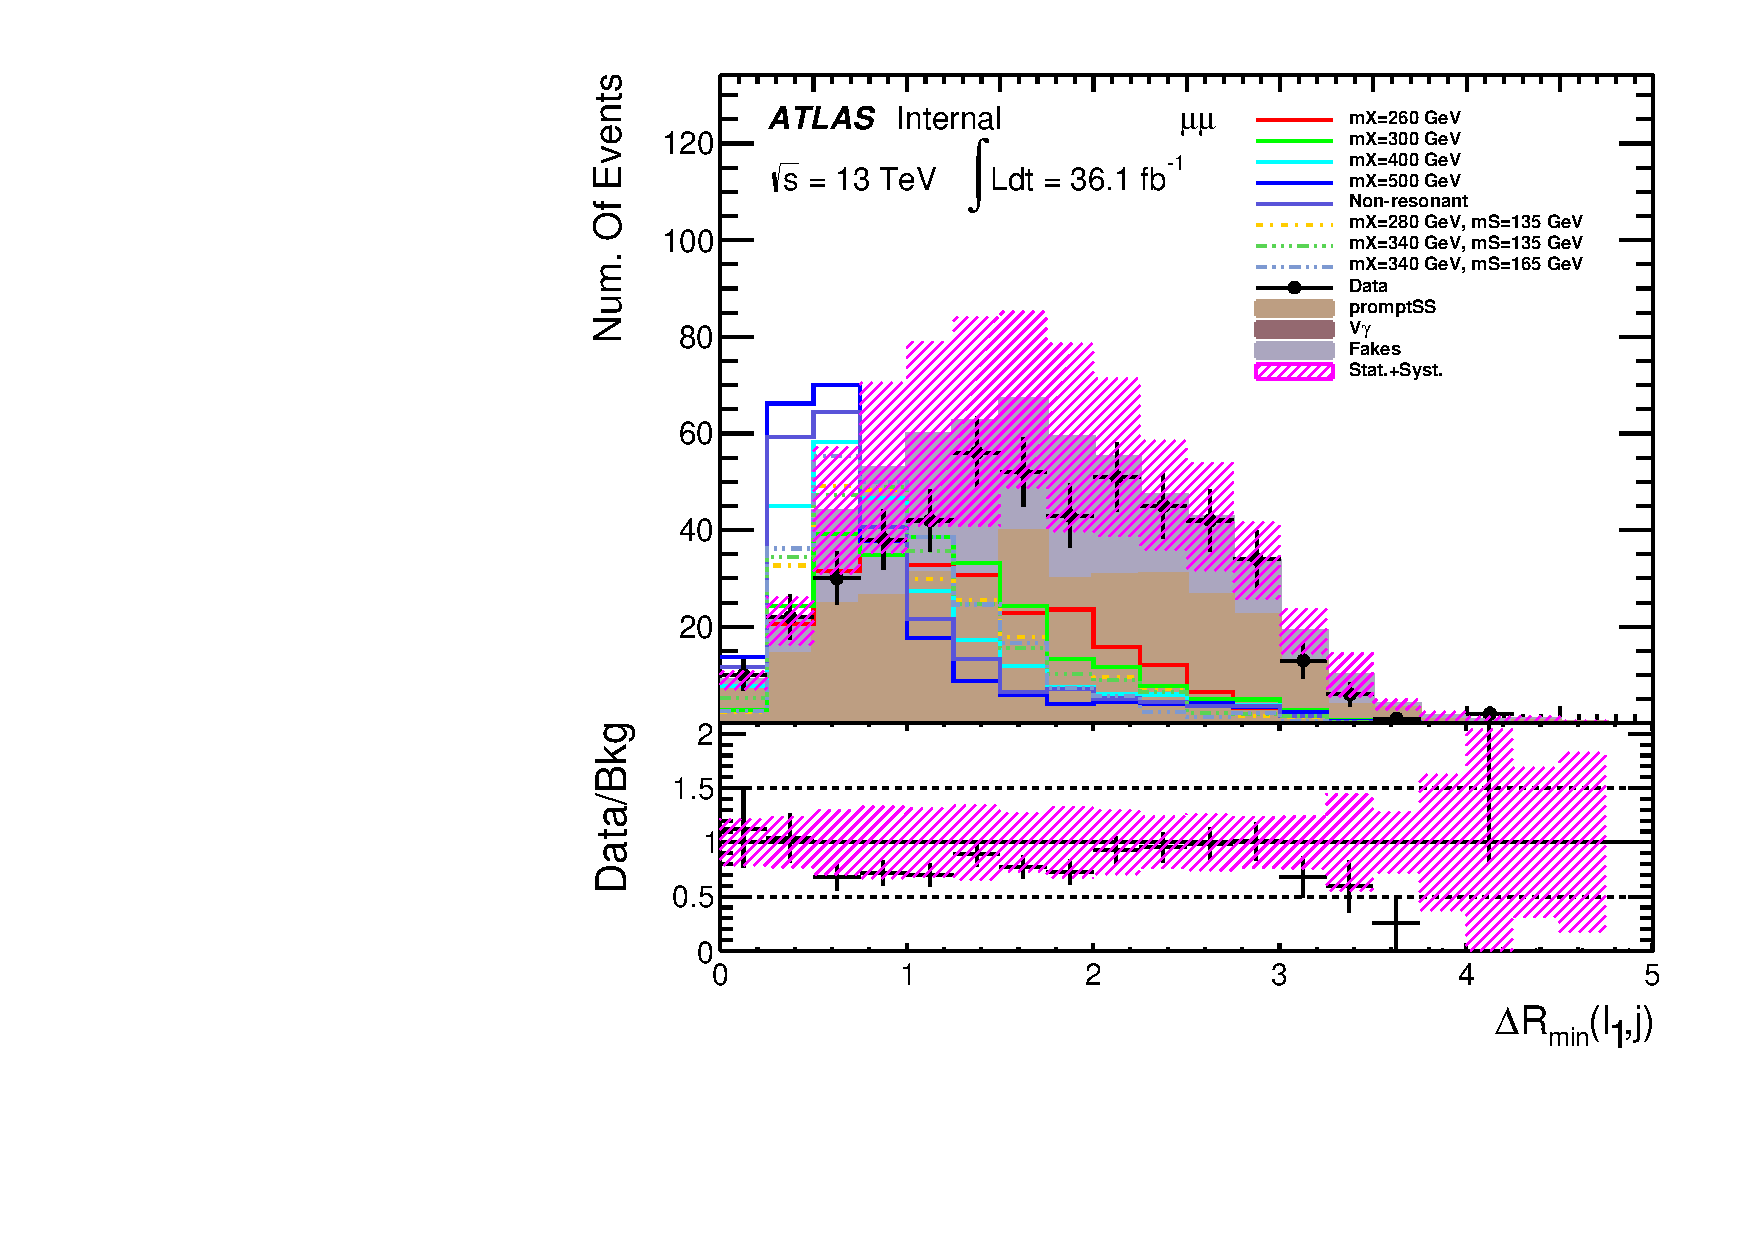
\includegraphics[width=1.0\textwidth]{fig/dataMC_low_Njet_CR/mindR_l1j_mumu.pdf}\label{fig:dataMC_low_Njet_CR:mindRl1j_mumu.pdf}
 \end{minipage}
 \begin{minipage}[t]{0.33\linewidth}
 \centering
 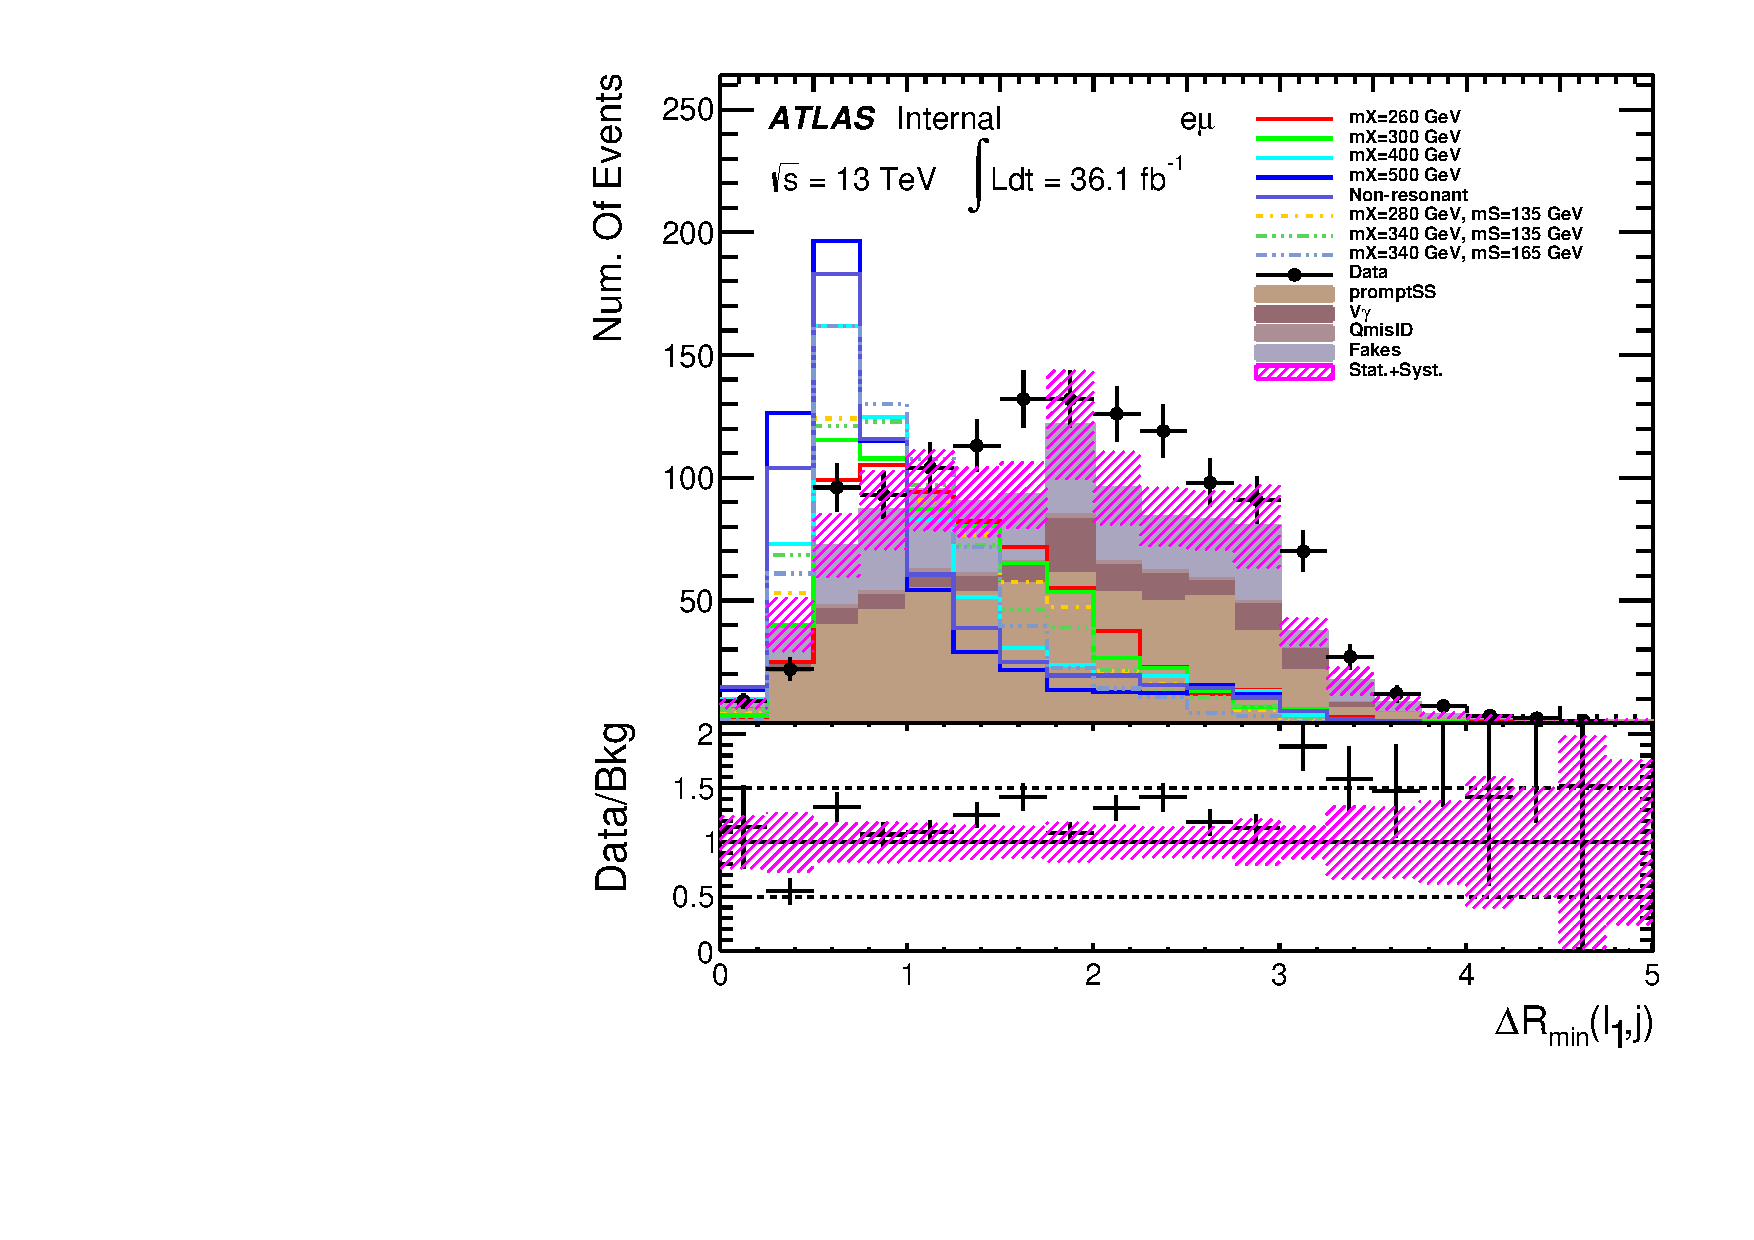
\includegraphics[width=1.0\textwidth]{fig/dataMC_low_Njet_CR/mindR_l1j_emu.pdf}\label{fig:dataMC_low_Njet_CR:mindRl1j_emu.pdf}
 \end{minipage}
 \begin{minipage}[t]{0.33\linewidth}
 \centering
 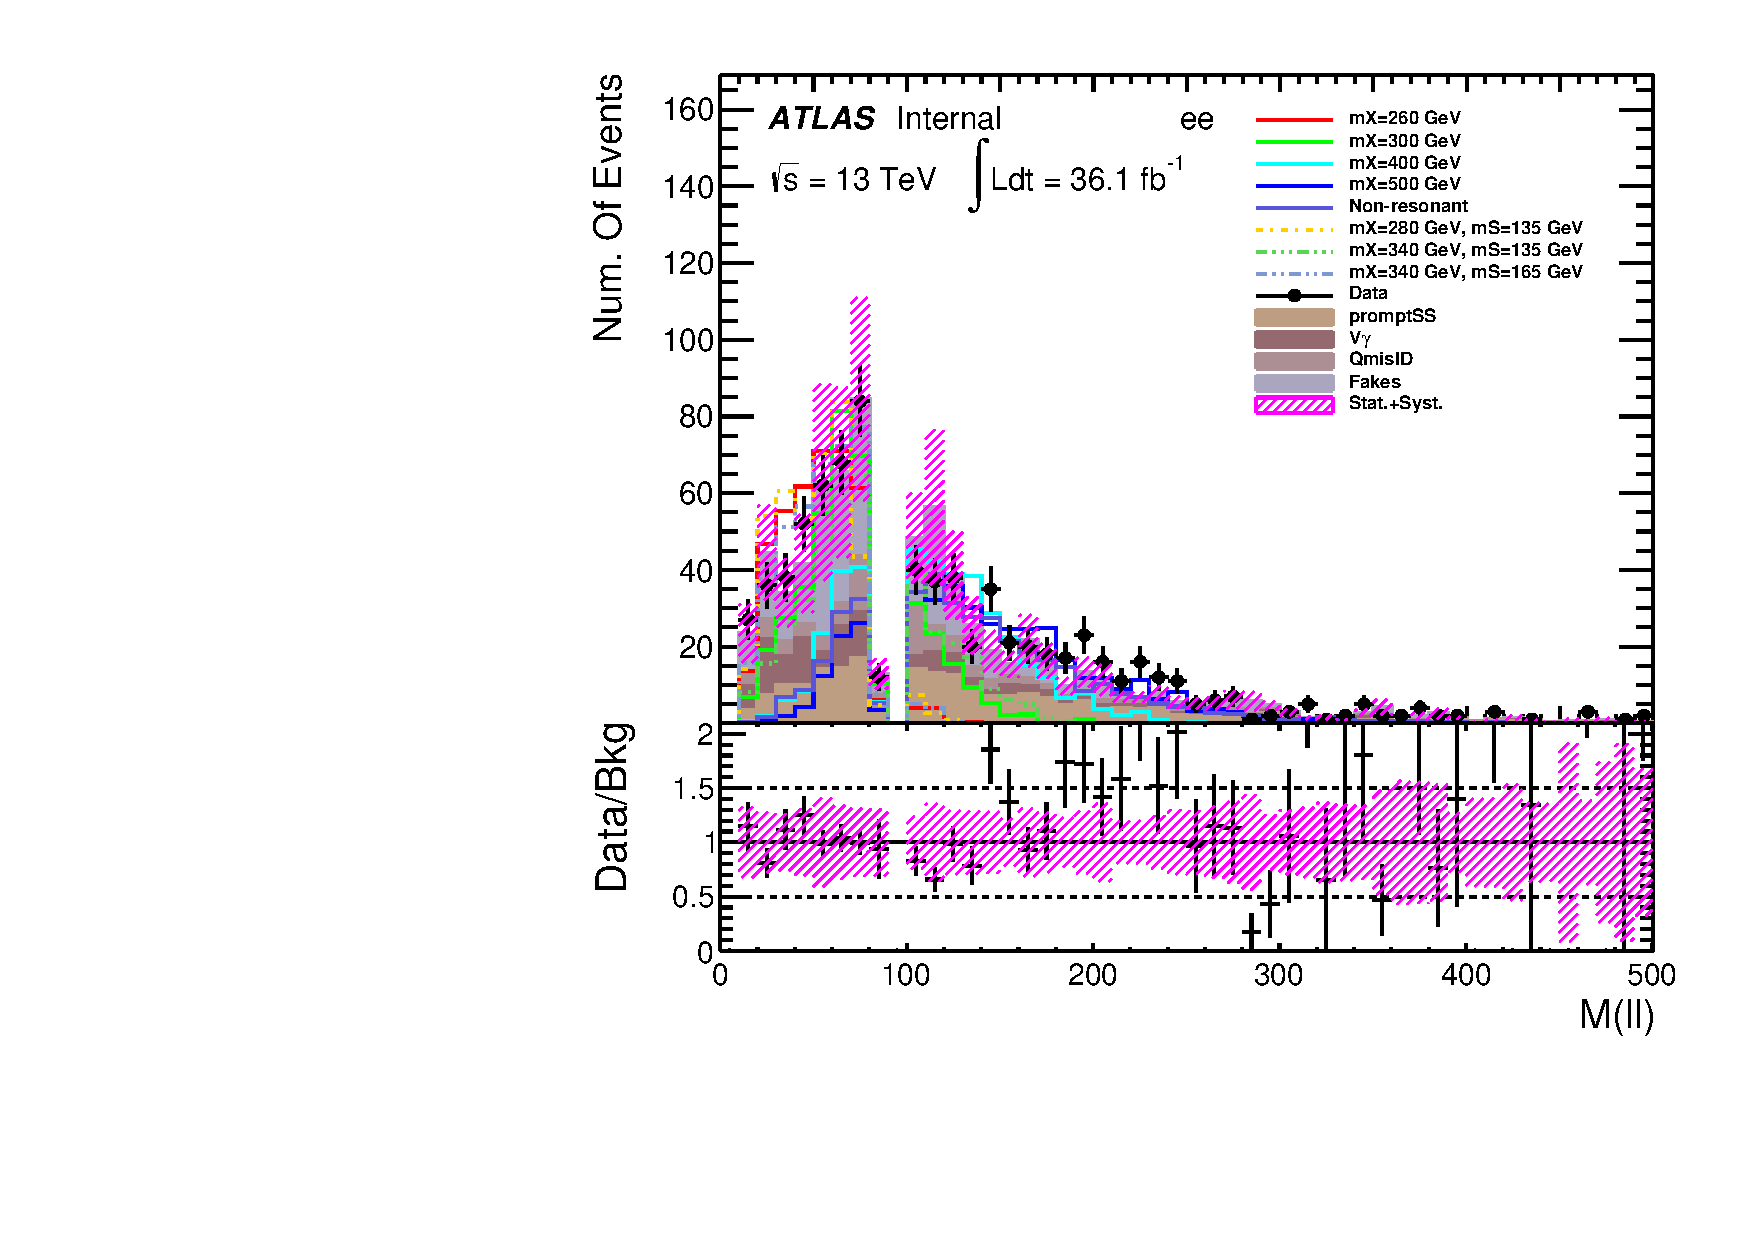
\includegraphics[width=1.0\textwidth]{fig/dataMC_low_Njet_CR/m_ll_ee.pdf}
 \label{fig:dataMC_low_Njet_CR:m_ll_ee.pdf}
 \end{minipage}
 \begin{minipage}[t]{0.33\linewidth}
 \centering
 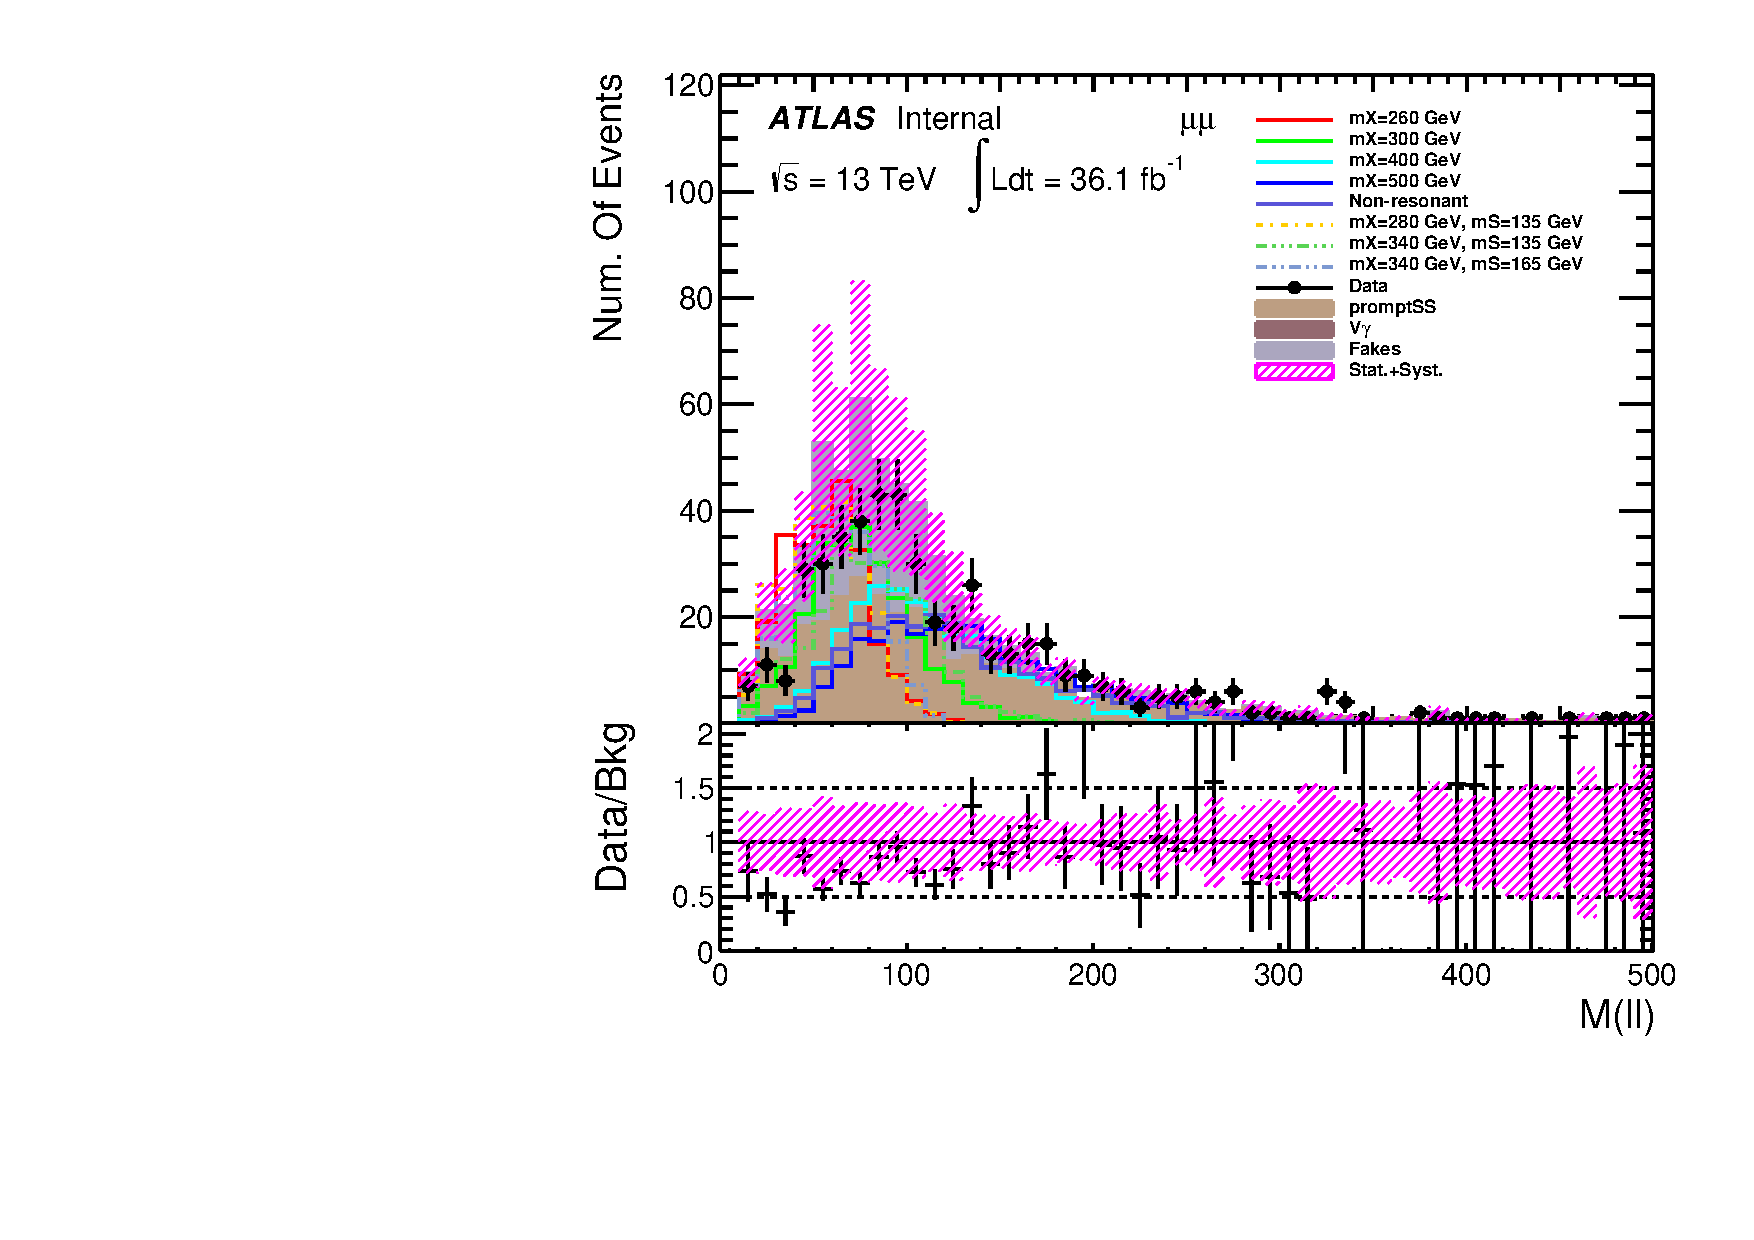
\includegraphics[width=1.0\textwidth]{fig/dataMC_low_Njet_CR/m_ll_mumu.pdf}
 \label{fig:dataMC_low_Njet_CR:m_ll_mumu.pdf}
 \end{minipage}
  \begin{minipage}[t]{0.33\linewidth}
 \centering
 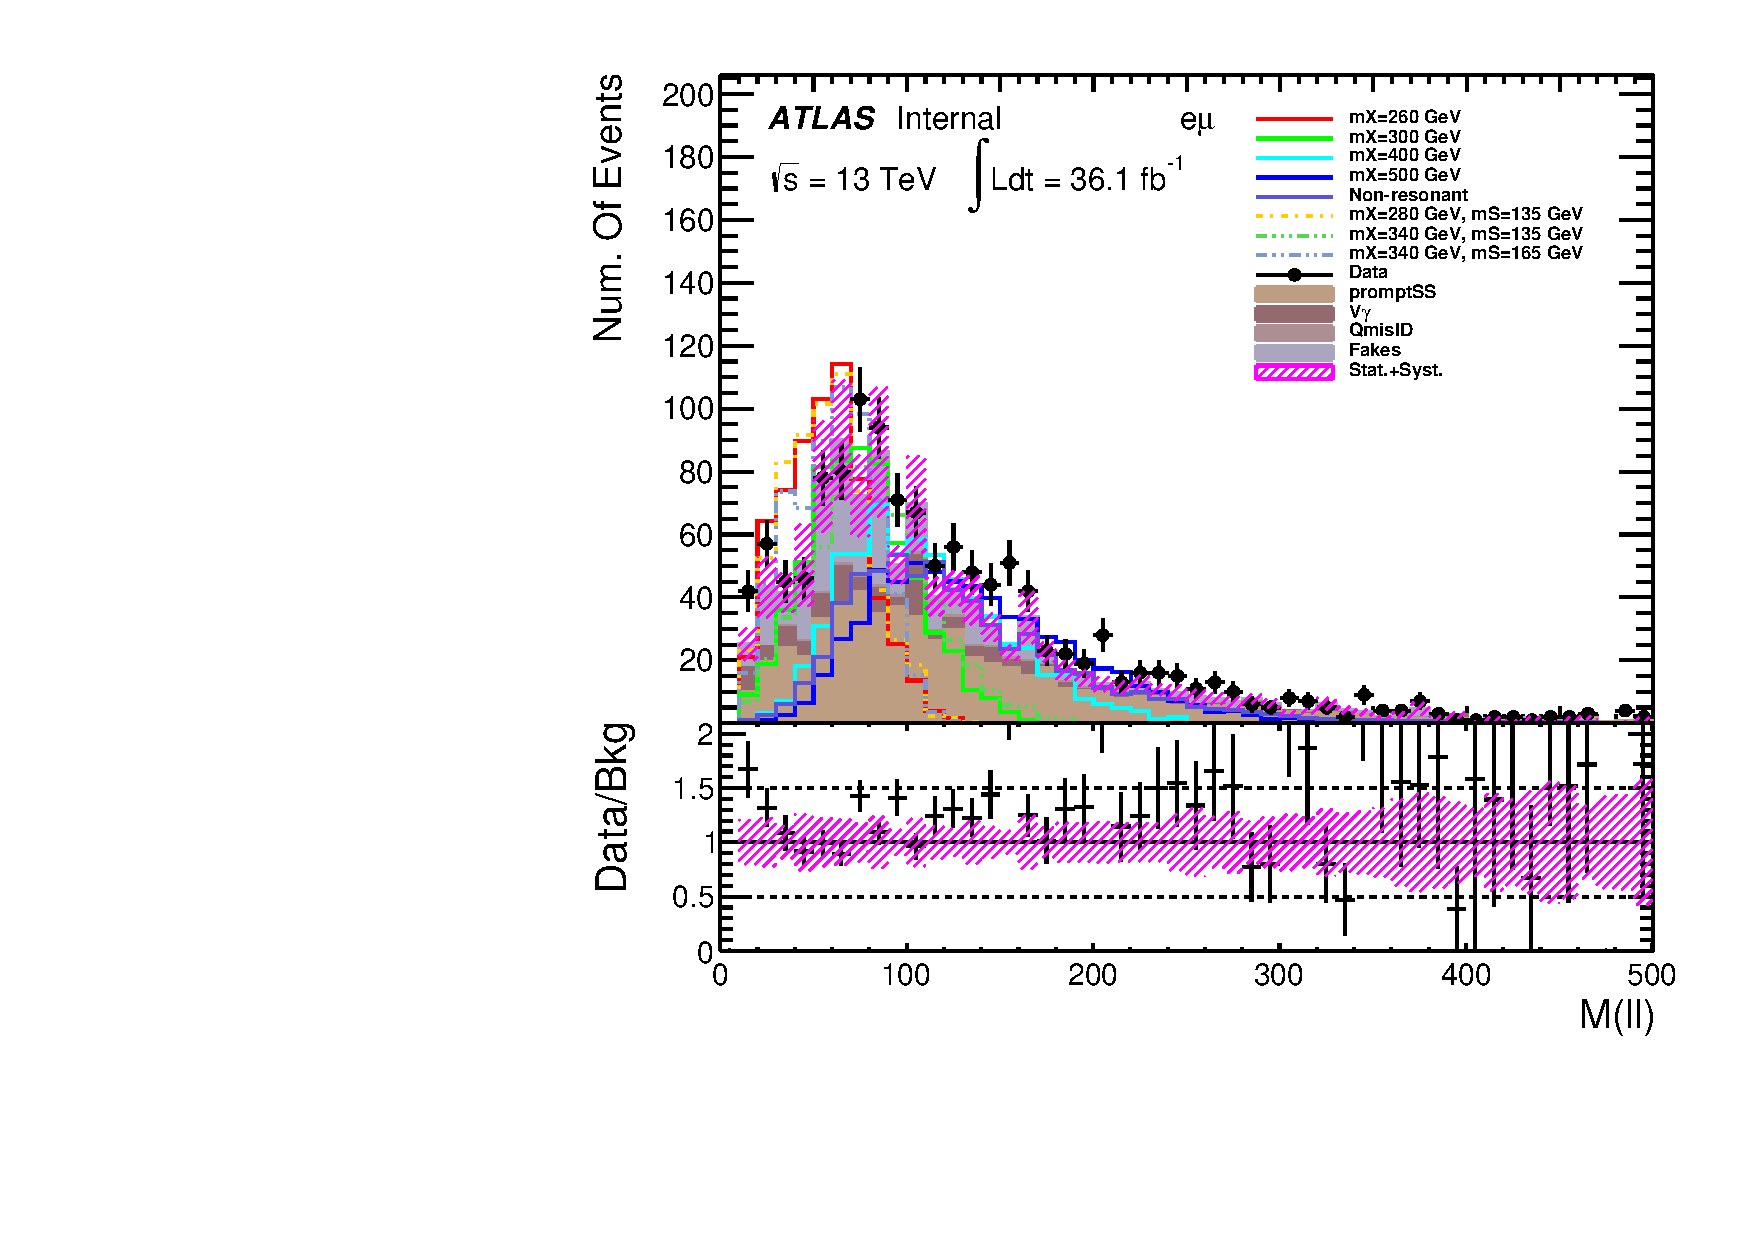
\includegraphics[width=1.0\textwidth]{fig/dataMC_low_Njet_CR/m_ll_emu.pdf}
 \label{fig:dataMC_low_Njet_CR:m_ll_emu.pdf}
 \end{minipage}
\begin{minipage}[t]{0.33\linewidth}
 \centering
 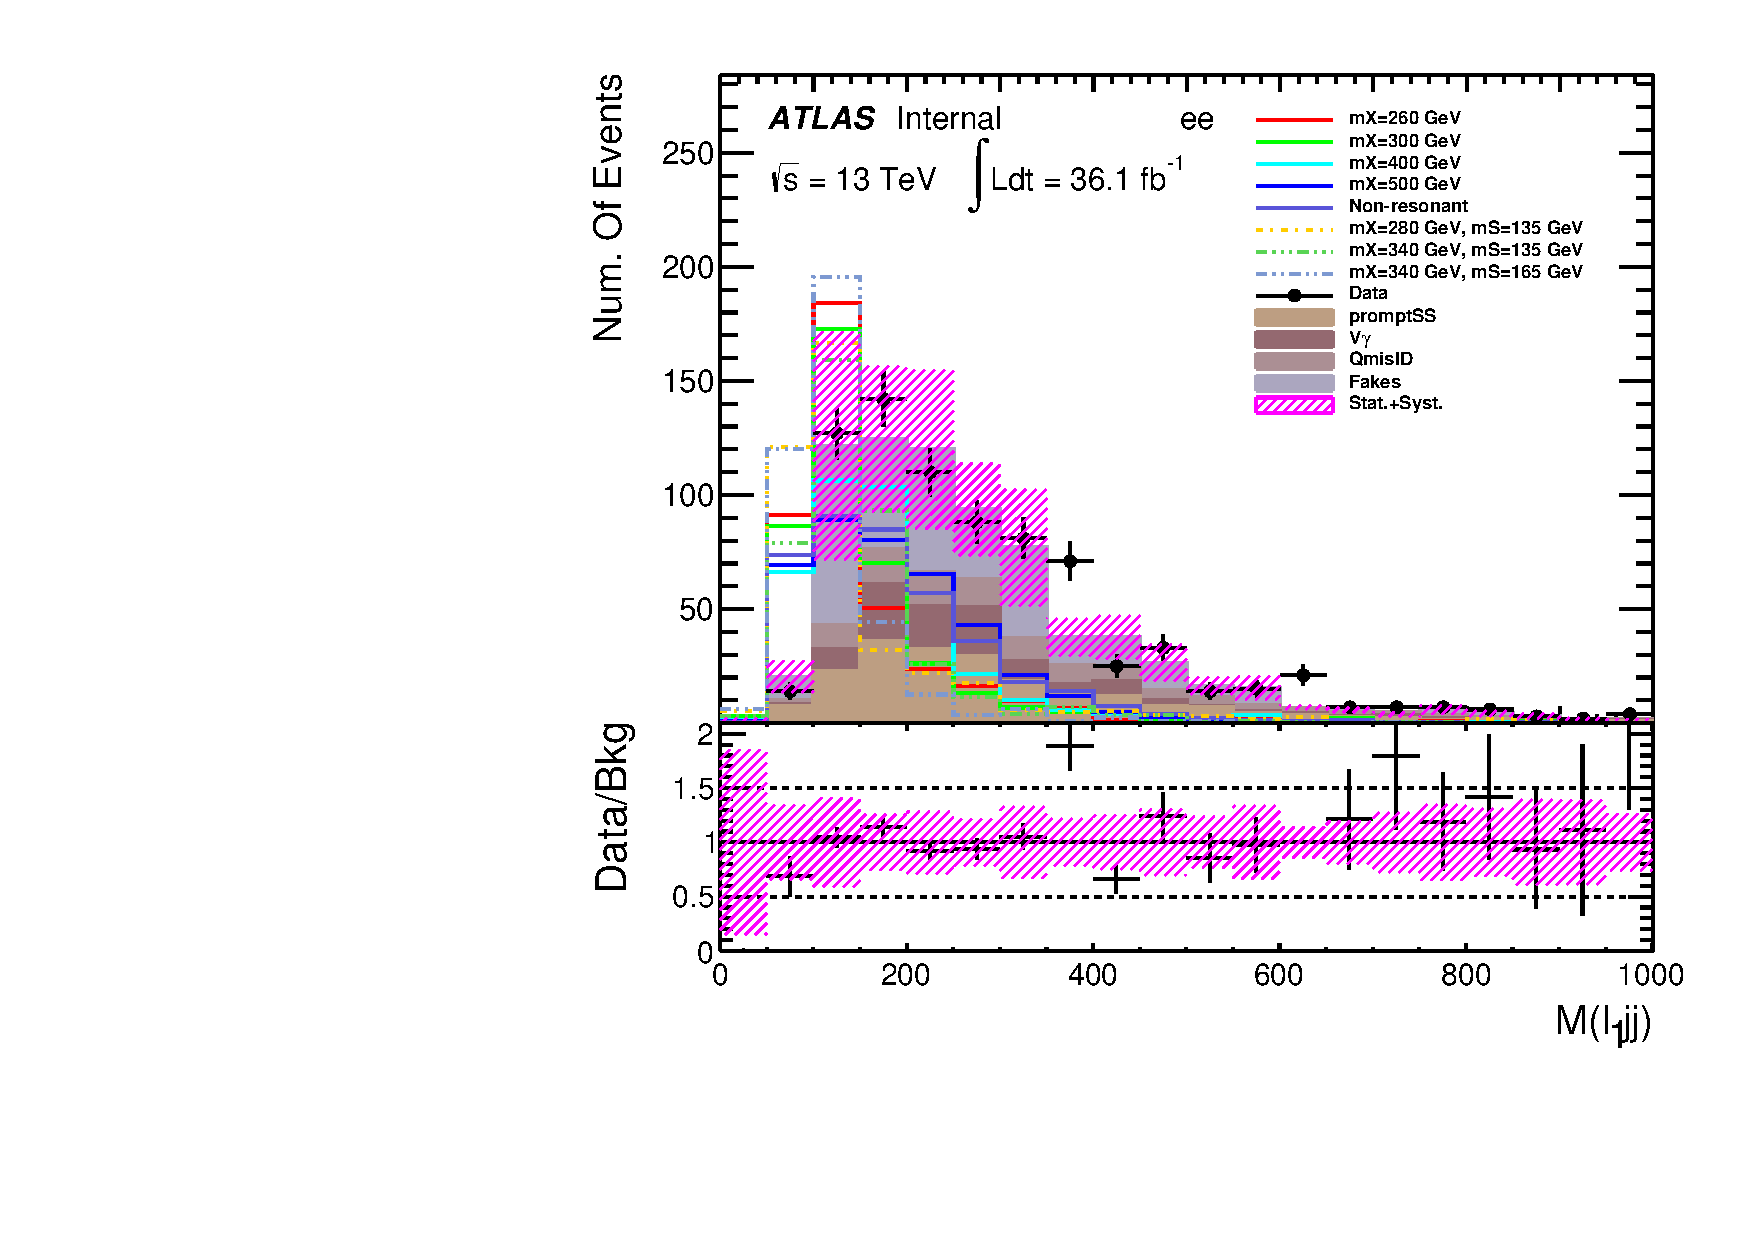
\includegraphics[width=1.0\textwidth]{fig/dataMC_low_Njet_CR/m_l1jj_ee.pdf}\label{fig:dataMC_low_Njet_CR:m_l1jj_ee.pdf}
 \end{minipage}
 \begin{minipage}[t]{0.33\linewidth}
 \centering
 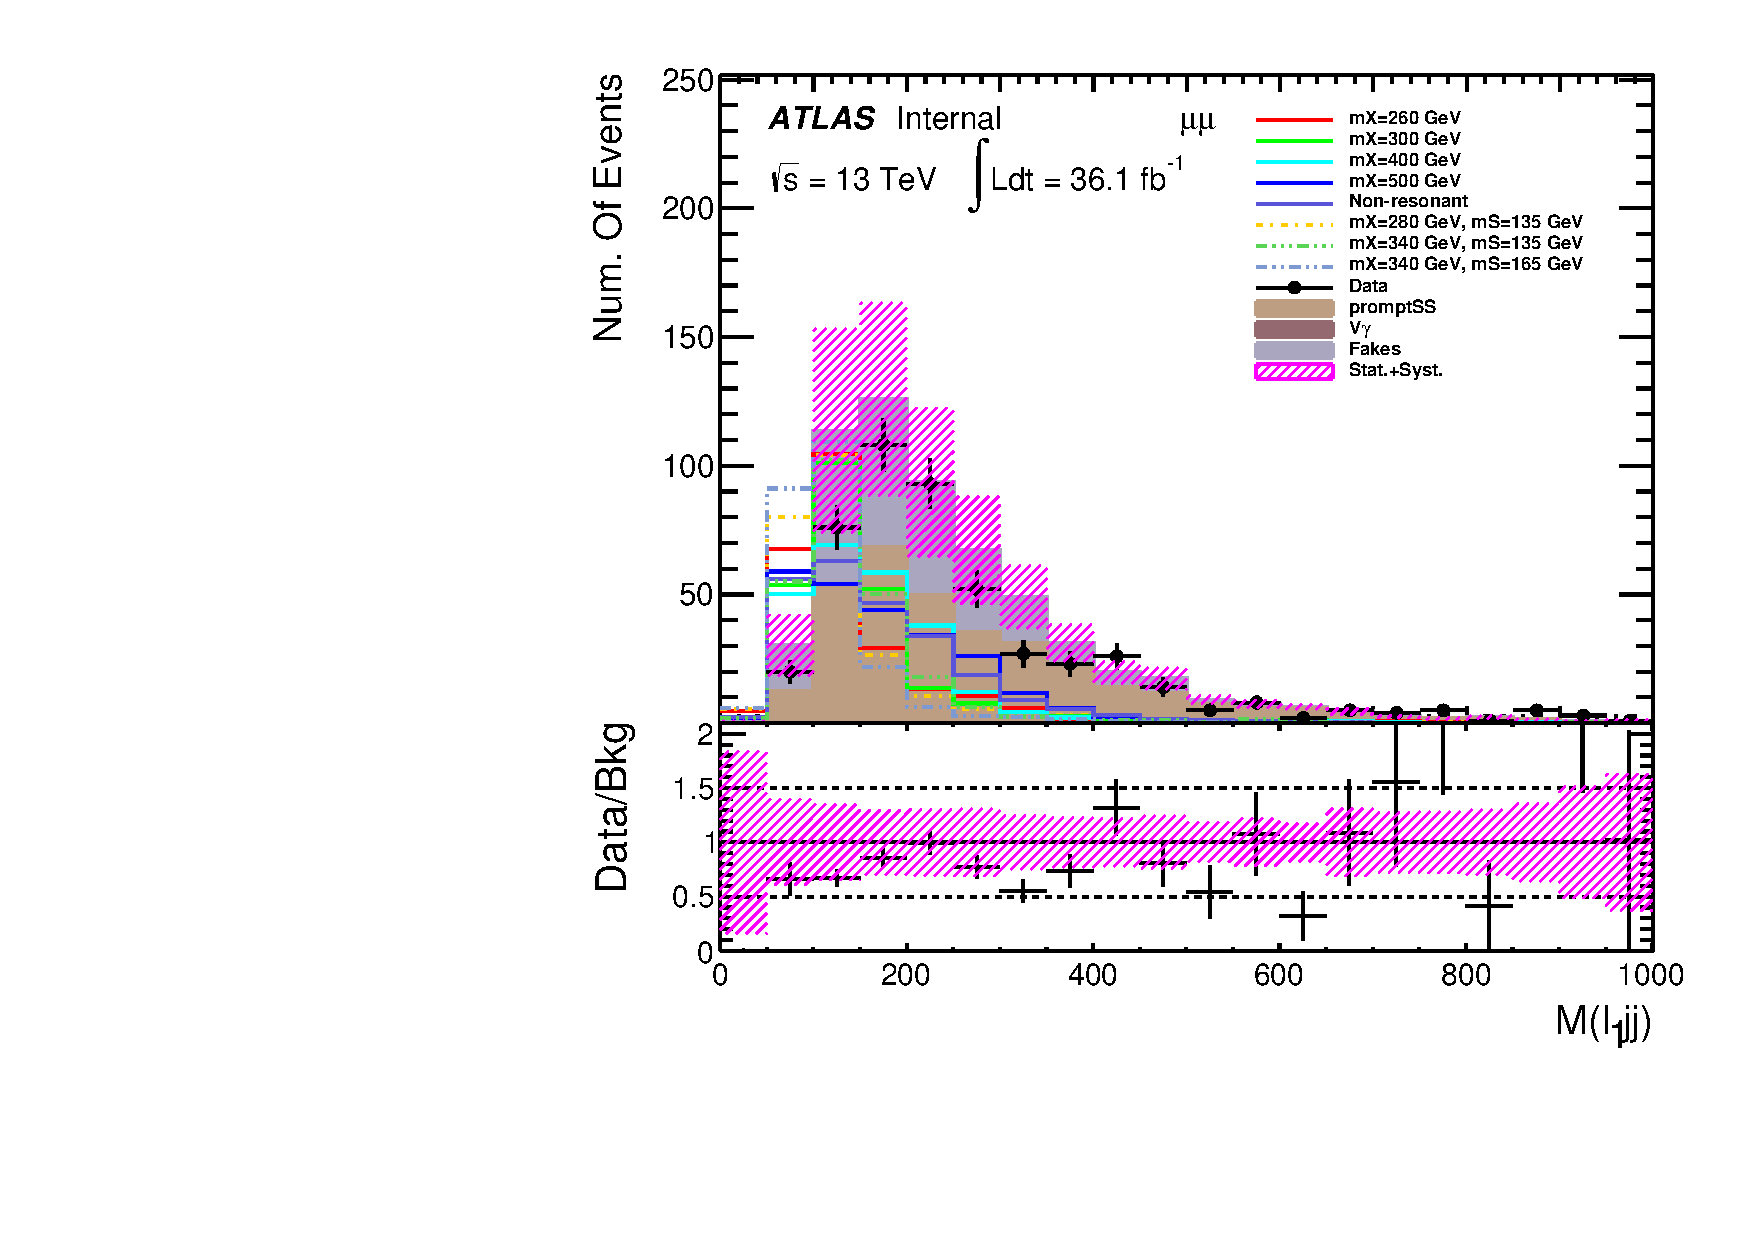
\includegraphics[width=1.0\textwidth]{fig/dataMC_low_Njet_CR/m_l1jj_mumu.pdf}\label{fig:dataMC_low_Njet_CR:m_l1jj_mumu.pdf}
 \end{minipage}
 \begin{minipage}[t]{0.33\linewidth}
 \centering
 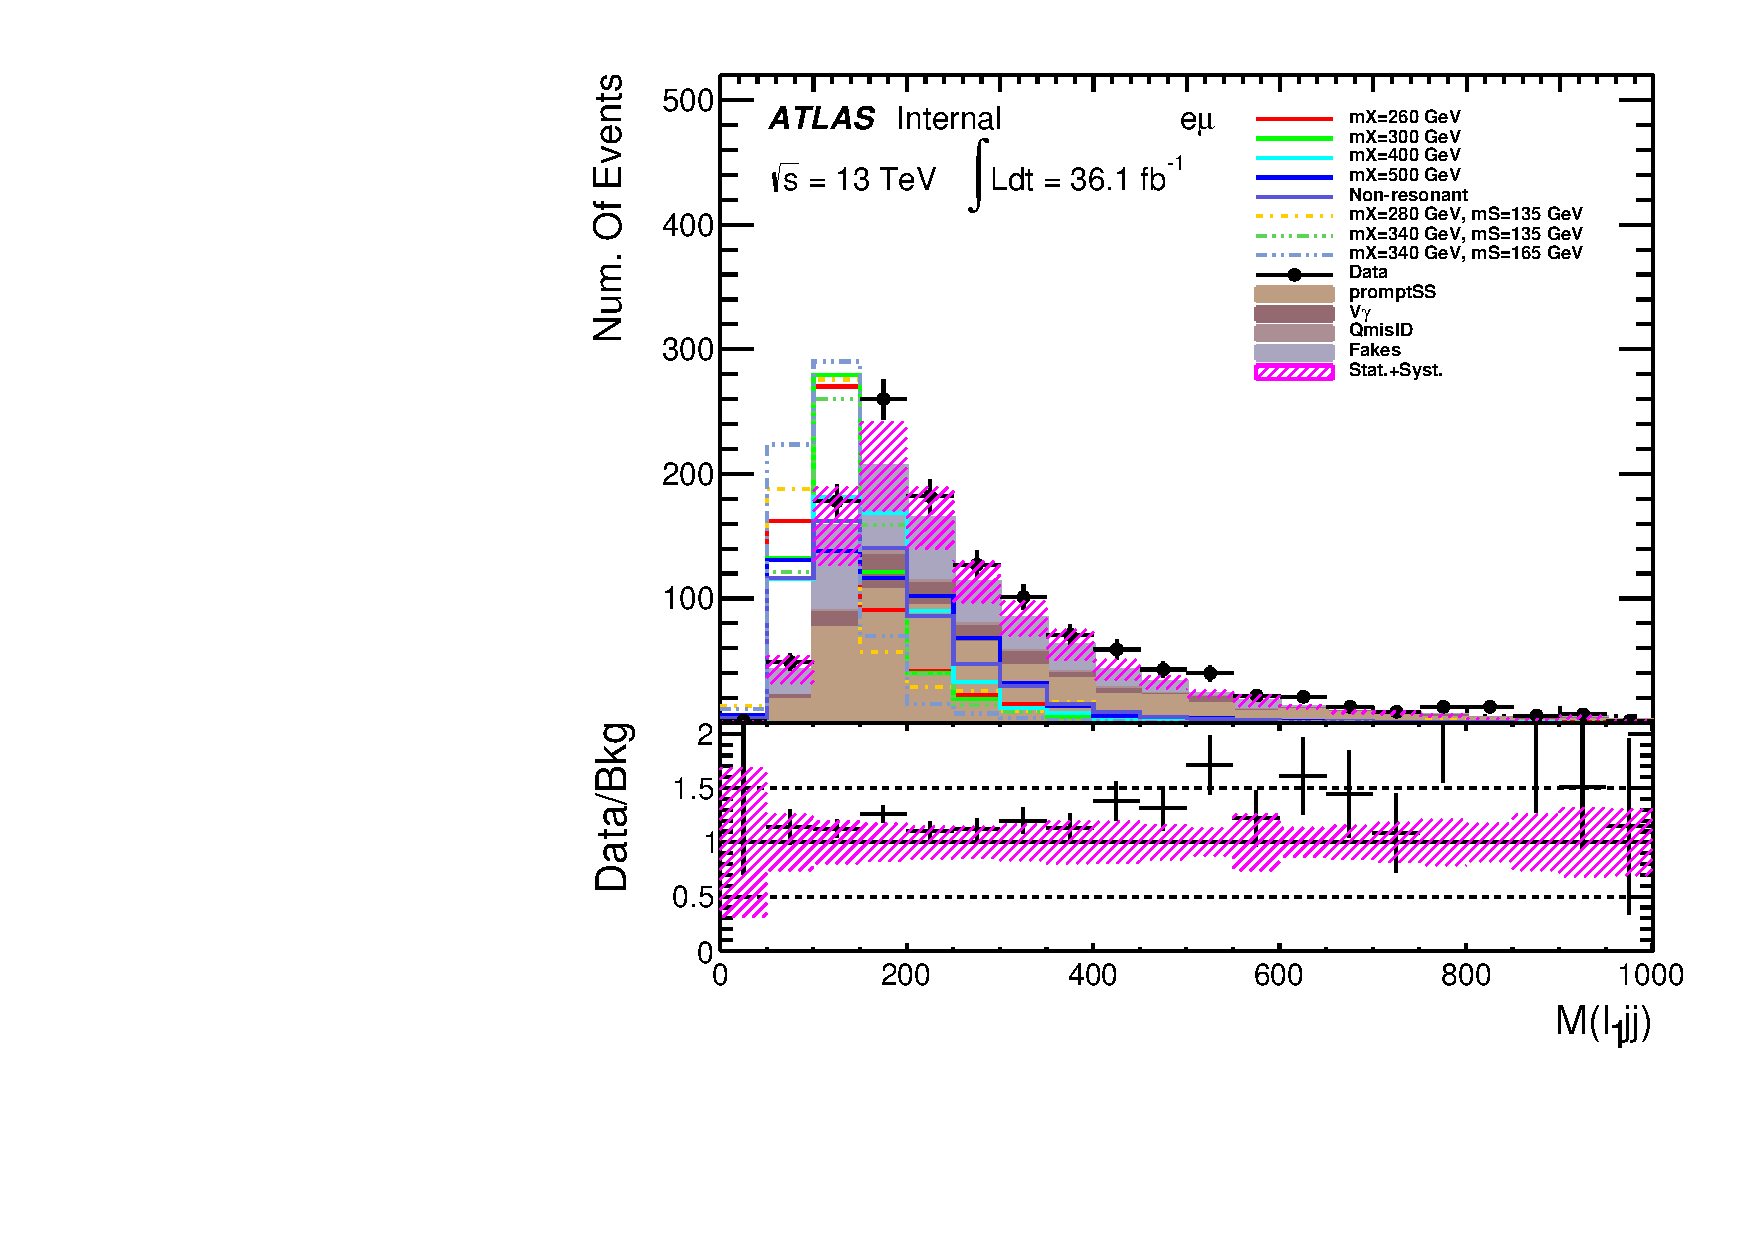
\includegraphics[width=1.0\textwidth]{fig/dataMC_low_Njet_CR/m_l1jj_emu.pdf}\label{fig:dataMC_low_Njet_CR:m_l1jj_emu.pdf}
 \end{minipage}
 \begin{minipage}[t]{0.33\linewidth}
 \centering
 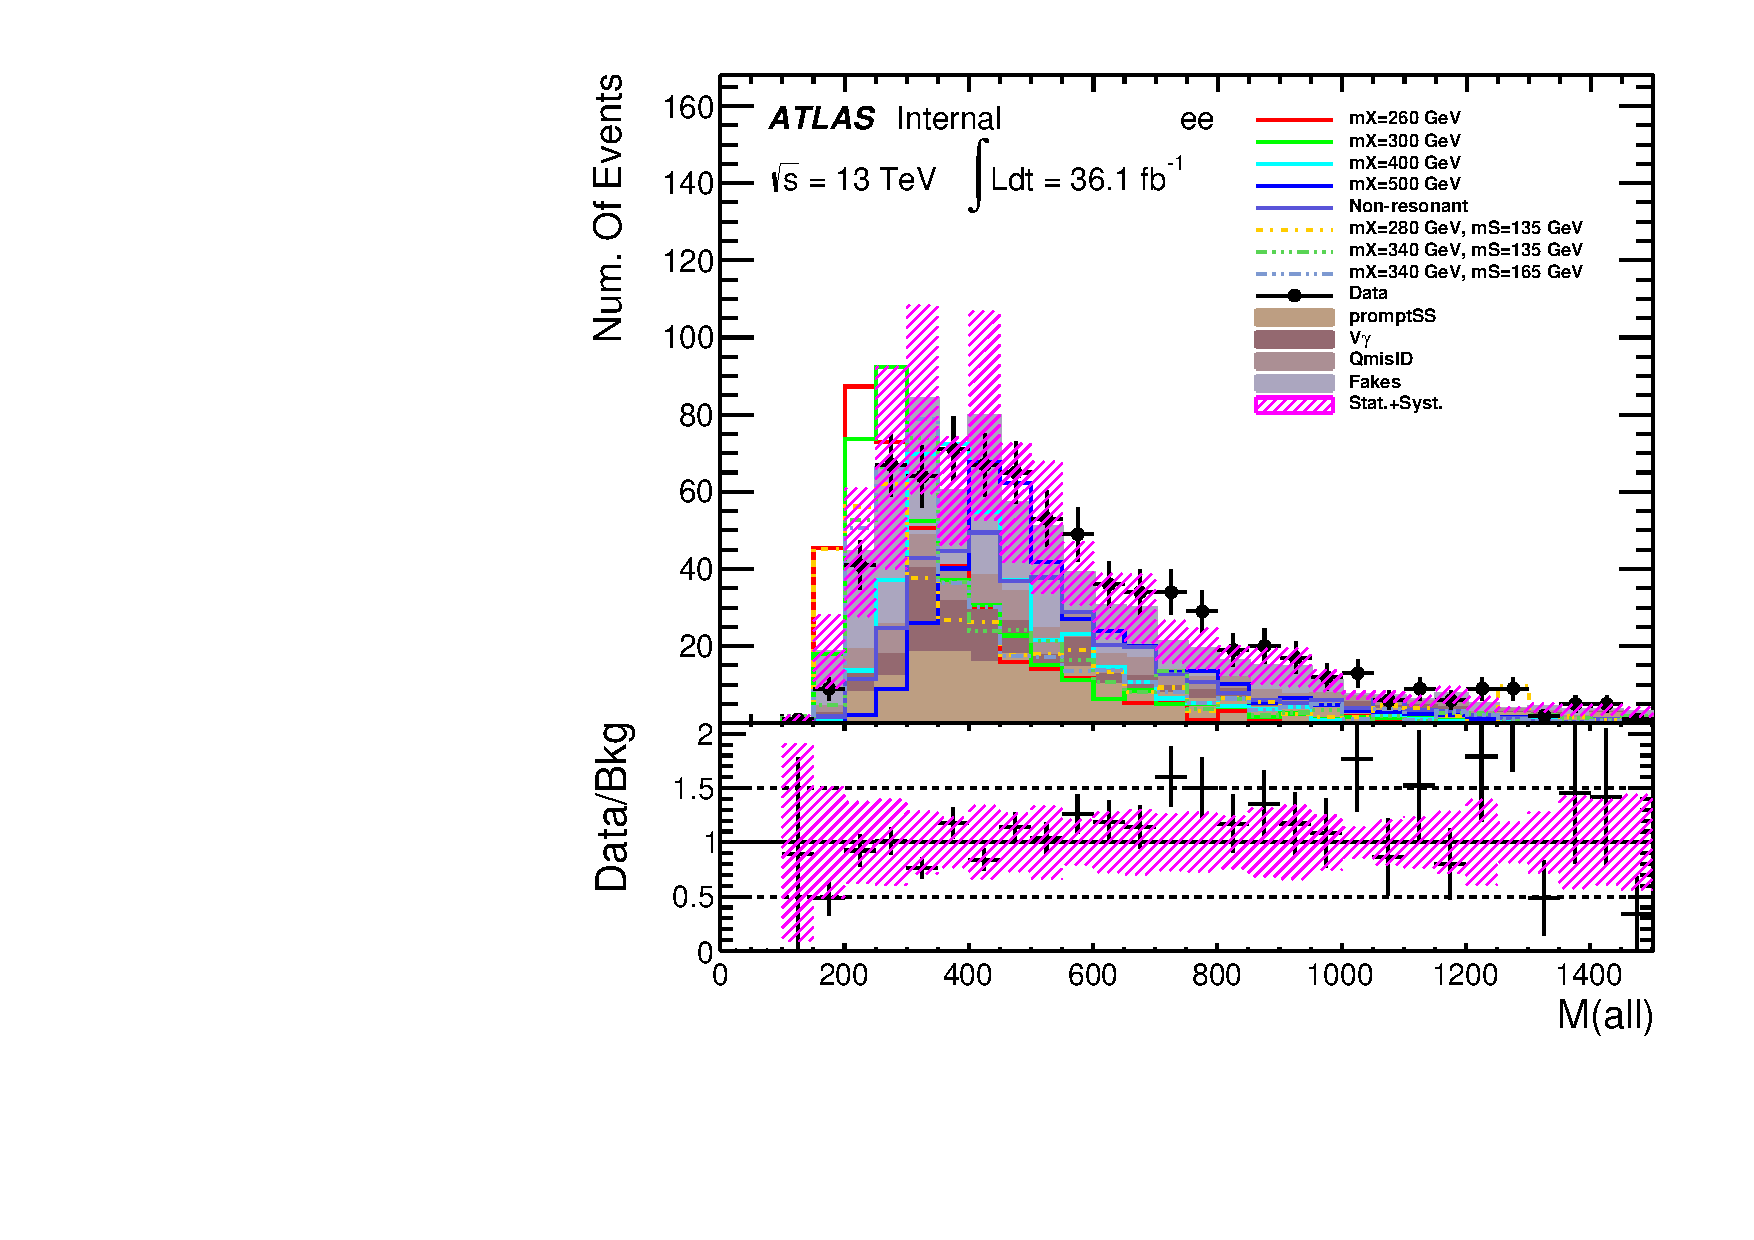
\includegraphics[width=1.0\textwidth]{fig/dataMC_low_Njet_CR/m_all_ee.pdf}\label{fig:dataMC_low_Njet_CR:m_all_ee.pdf}
 \end{minipage}
  \begin{minipage}[t]{0.33\linewidth}
 \centering
 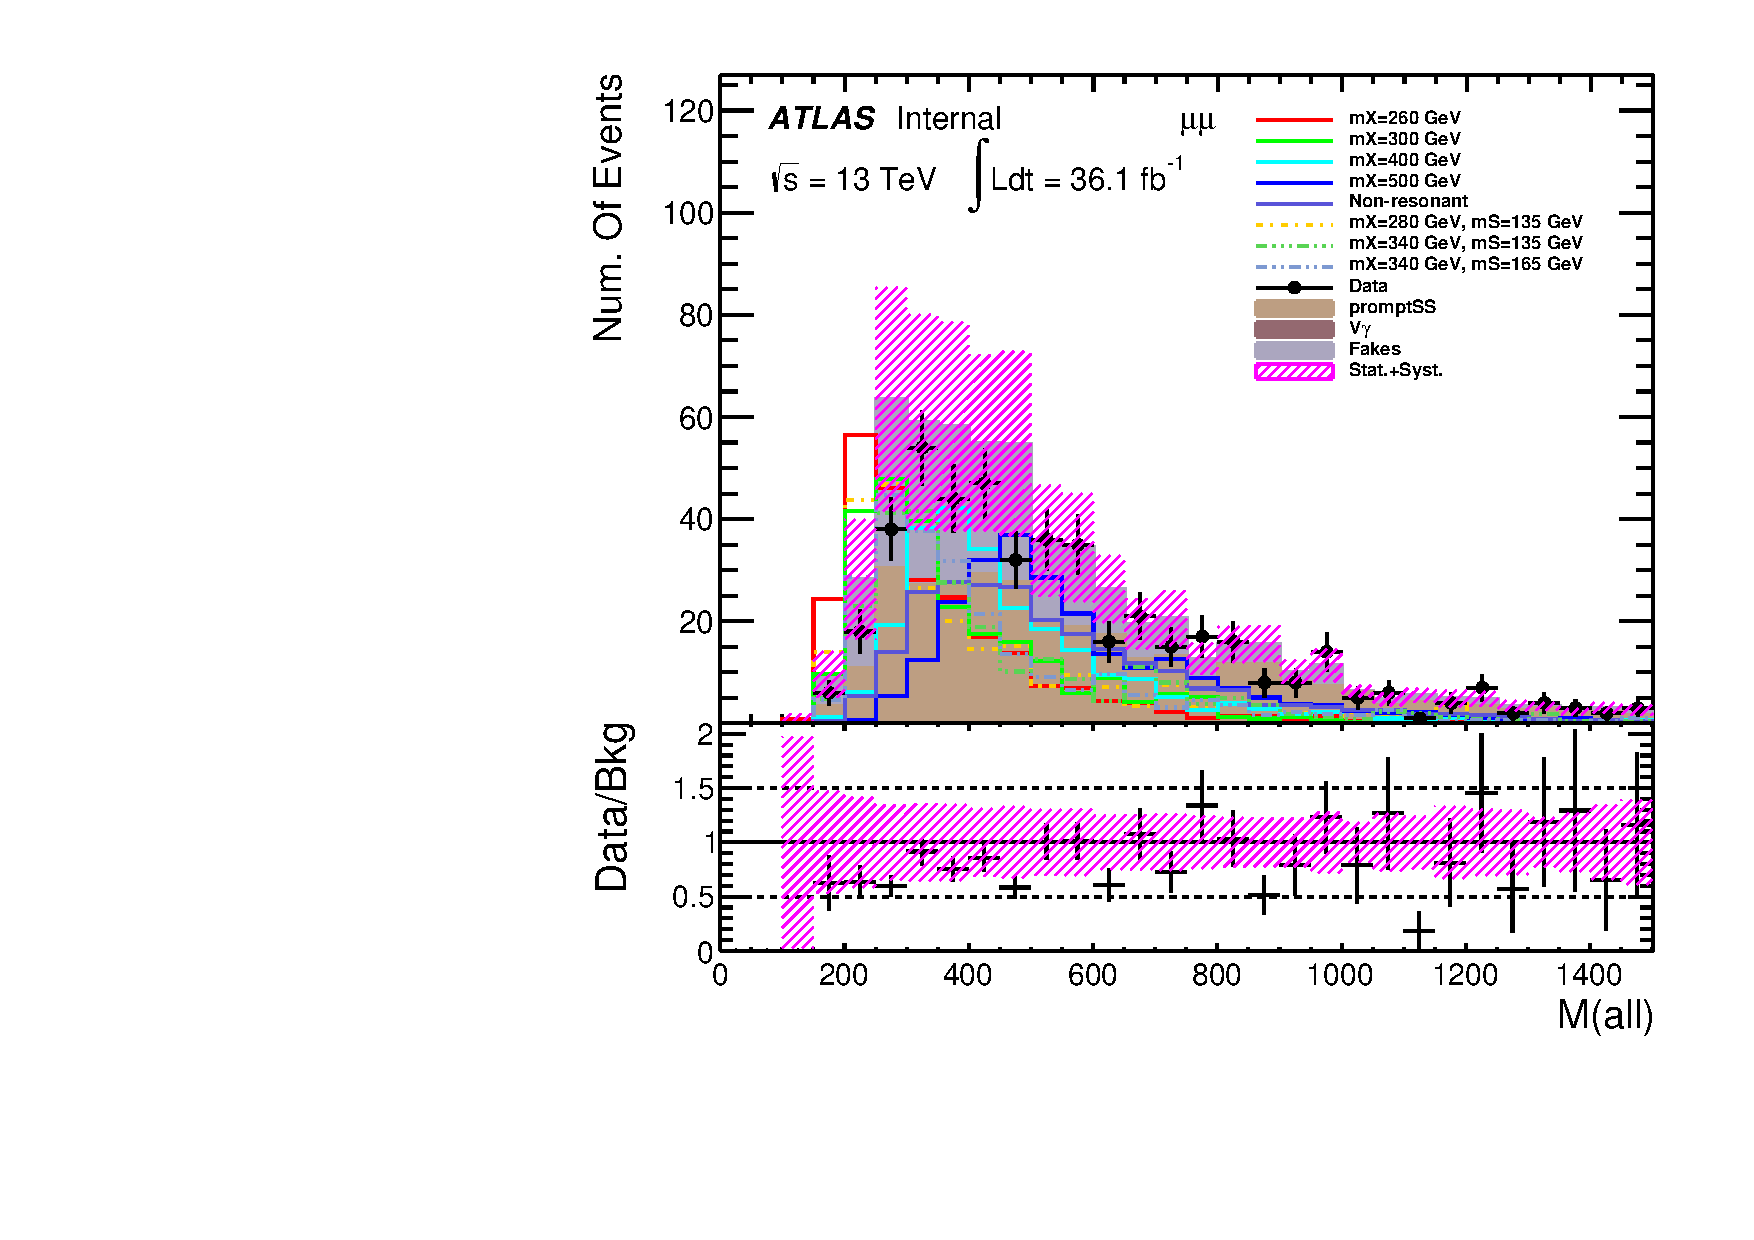
\includegraphics[width=1.0\textwidth]{fig/dataMC_low_Njet_CR/m_all_mumu.pdf}\label{fig:dataMC_low_Njet_CR:m_all_mumu.pdf}
 \end{minipage}
 \begin{minipage}[t]{0.33\linewidth}
 \centering
 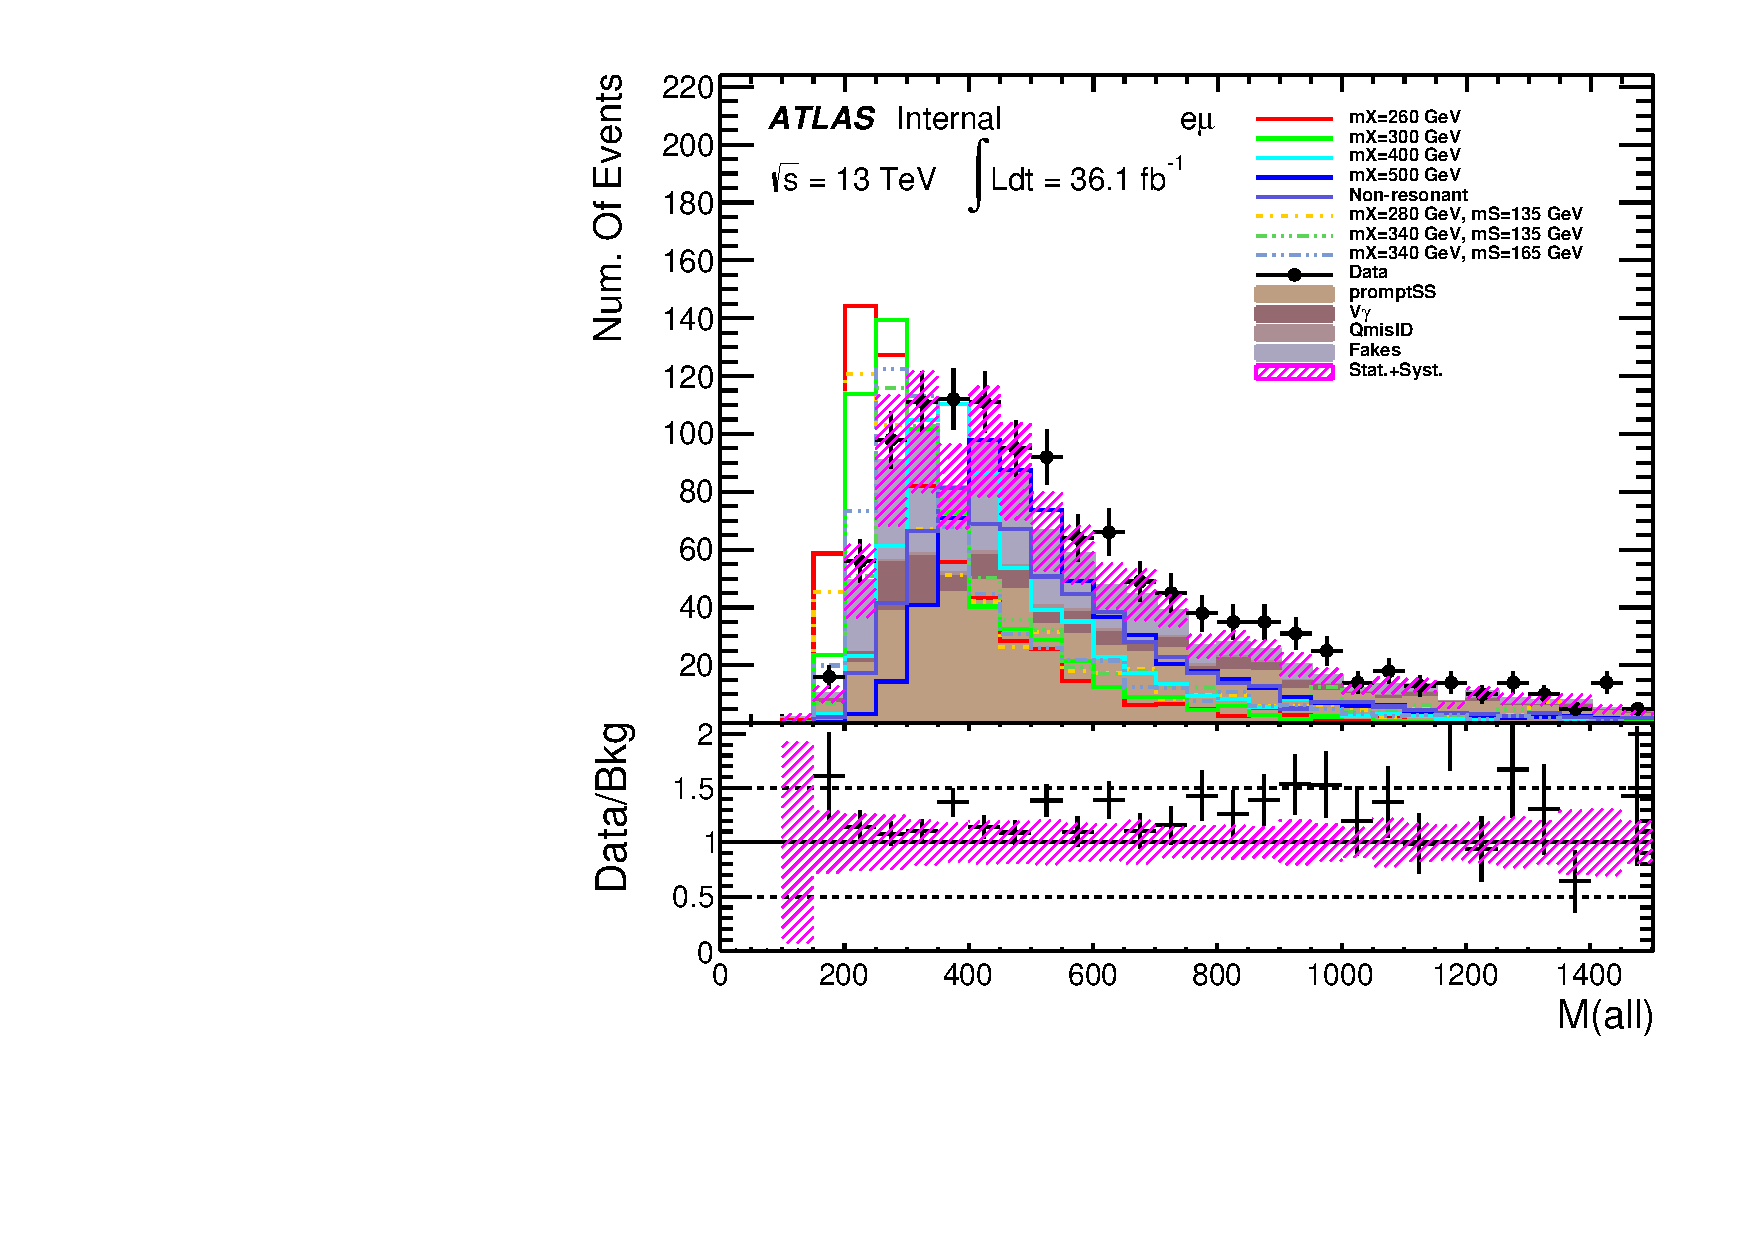
\includegraphics[width=1.0\textwidth]{fig/dataMC_low_Njet_CR/m_all_emu.pdf}\label{fig:dataMC_low_Njet_CR:m_all_emu.pdf}
 \end{minipage}
 \caption{The distributions of kinematic variables that are used to form optimization selections at pre-selection level, corresponding to $N_{\text{jet}}\geq2$. Left: $ee$, middle: $\mu\mu$, right: $e\mu$. PromptSS and $V+\gamma$ are normalized to the luminosity of 36.1 fb$^{-1}$.}
\label{fig:SigOpt_low_kine}
\end{figure}

\begin{figure}[h]
 \begin{minipage}[t]{0.33\linewidth}
 \centering
 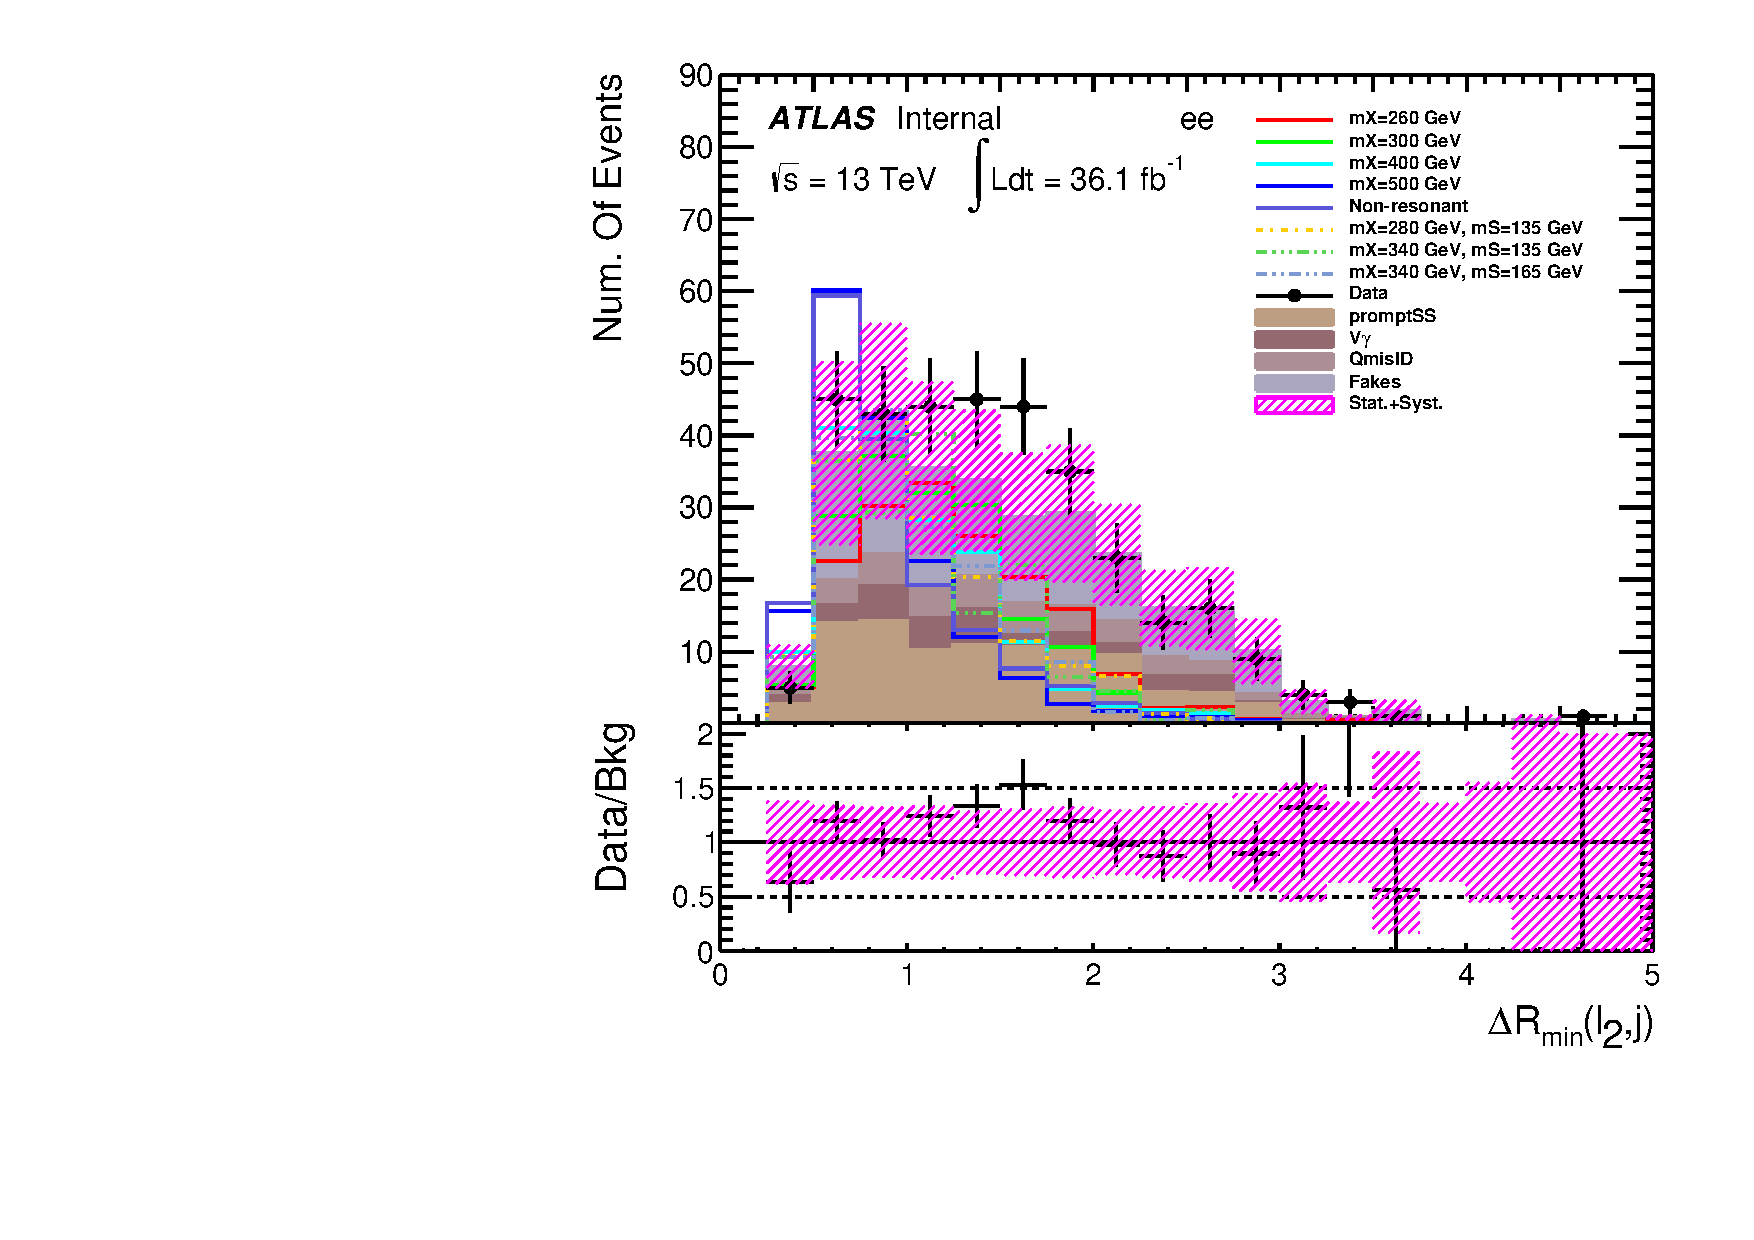
\includegraphics[width=1.0\textwidth]{fig/dataMC_high_Njet_CR/mindR_l2j_ee.pdf}\label{fig:dataMC_high_Njet_CR:mindRl2j_ee.pdf}
 \end{minipage}
 \begin{minipage}[t]{0.33\linewidth}
 \centering
 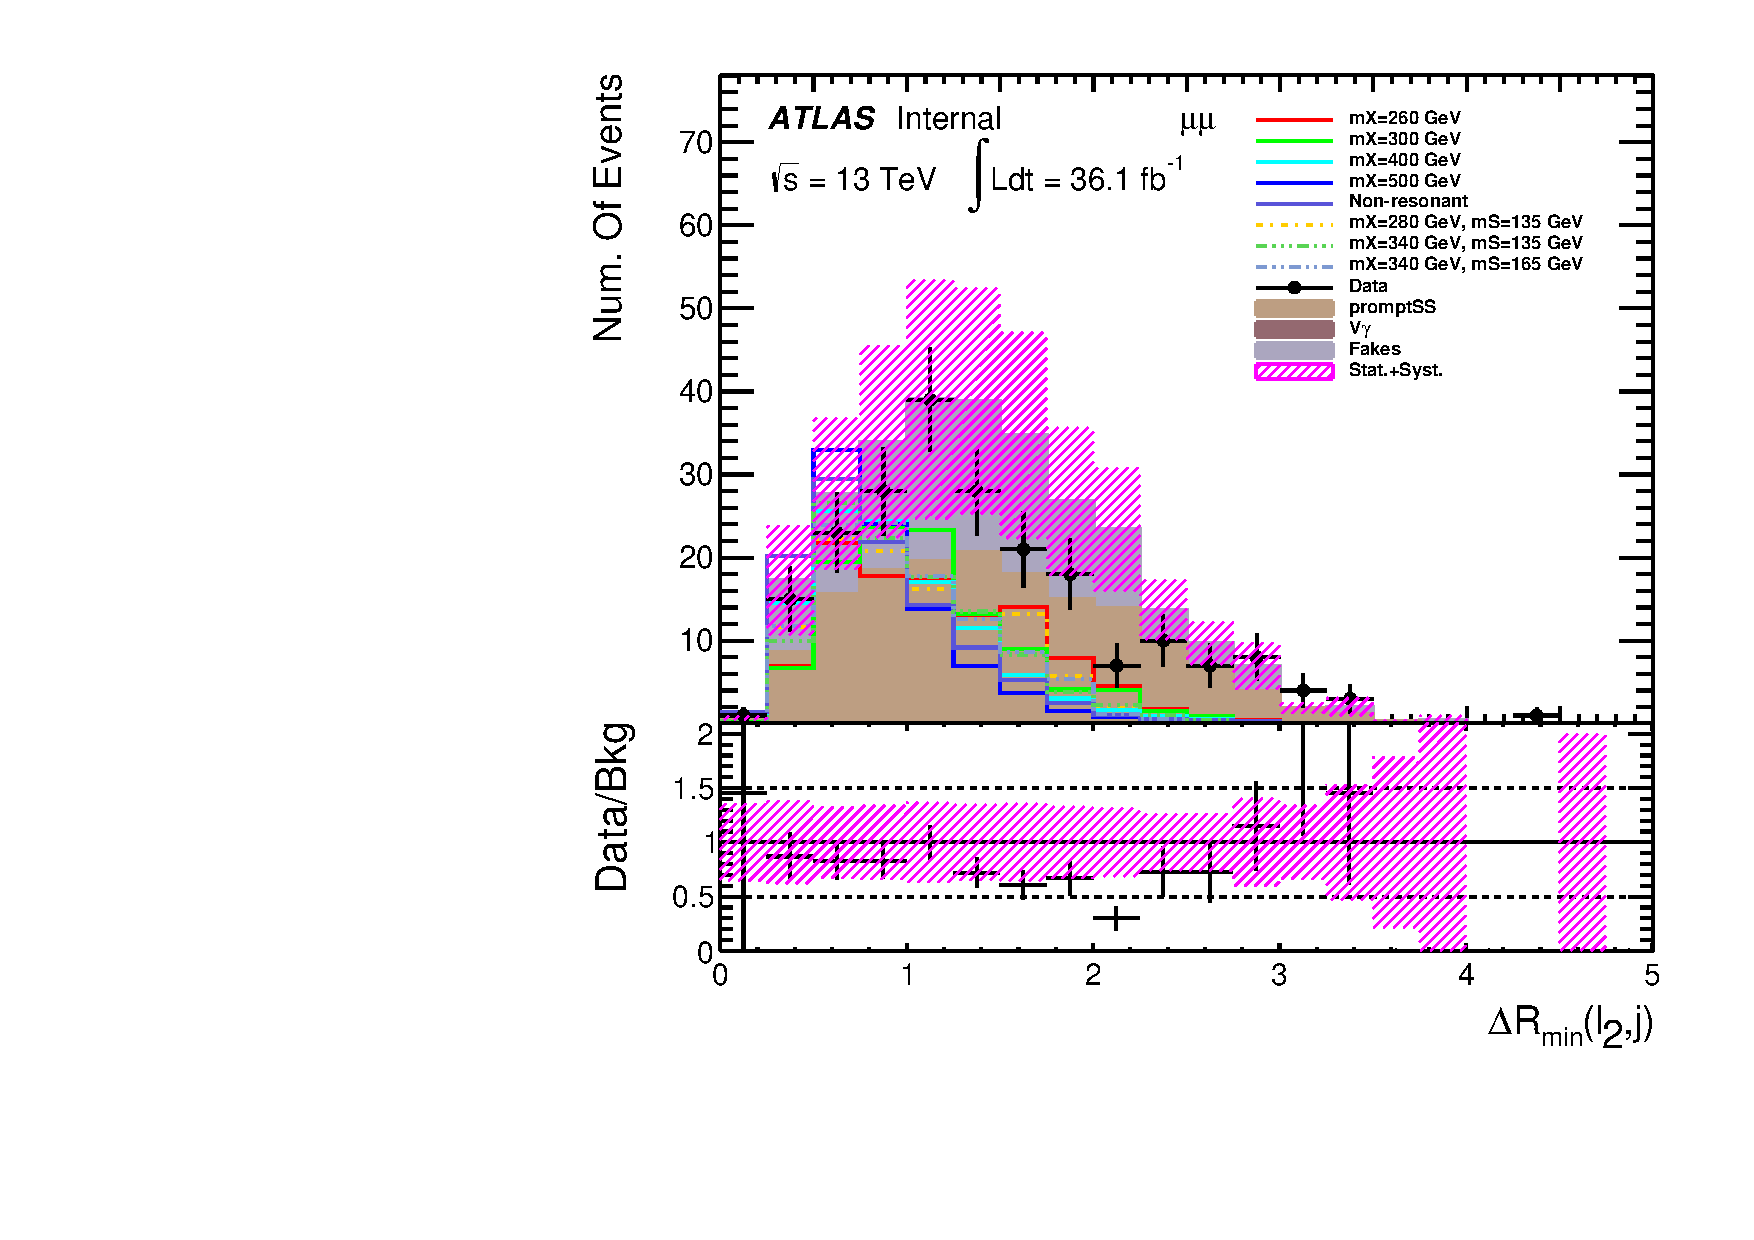
\includegraphics[width=1.0\textwidth]{fig/dataMC_high_Njet_CR/mindR_l2j_mumu.pdf}\label{fig:dataMC_high_Njet_CR:mindRl2j_mumu.pdf}
 \end{minipage}
 \begin{minipage}[t]{0.33\linewidth}
 \centering
 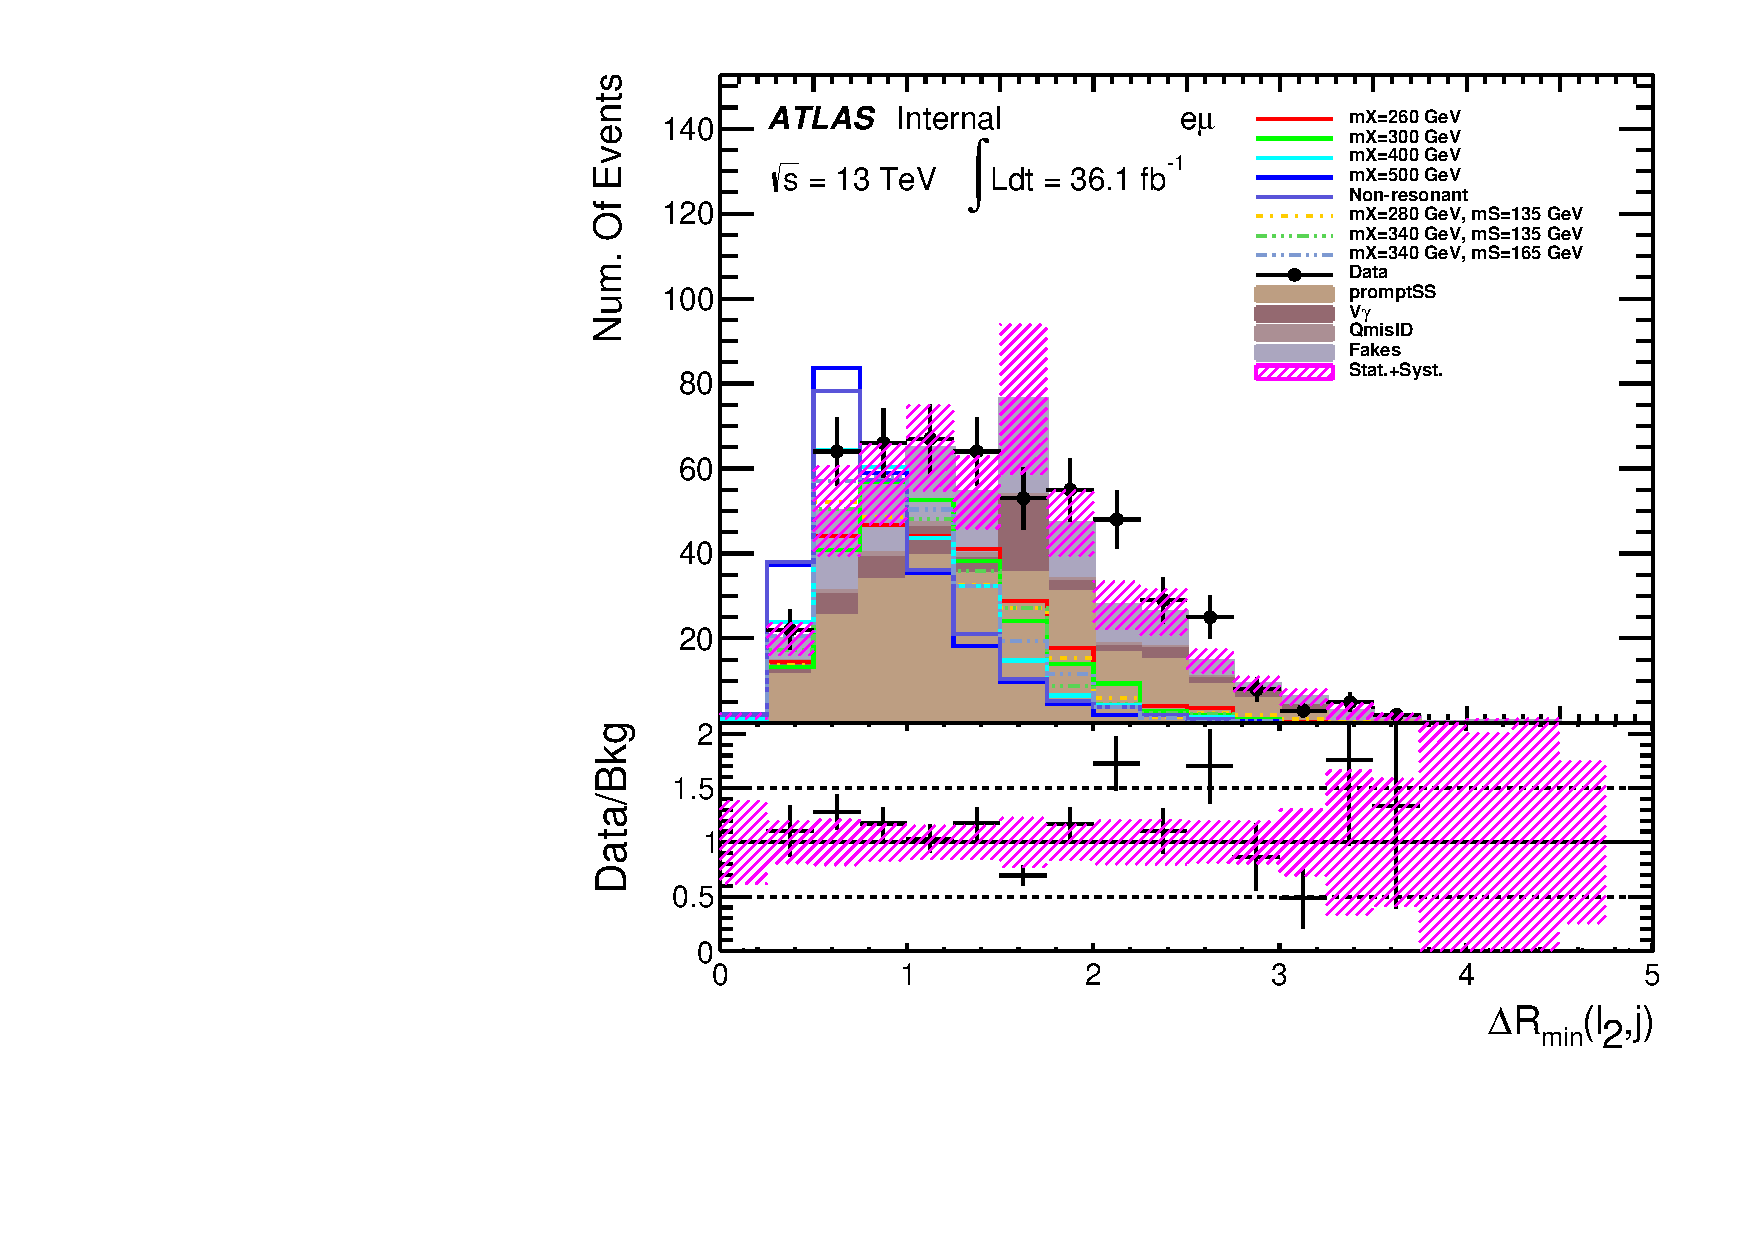
\includegraphics[width=1.0\textwidth]{fig/dataMC_high_Njet_CR/mindR_l2j_emu.pdf}\label{fig:dataMC_high_Njet_CR:mindRl2j_emu.pdf}
 \end{minipage}
 \begin{minipage}[t]{0.33\linewidth}
 \centering
 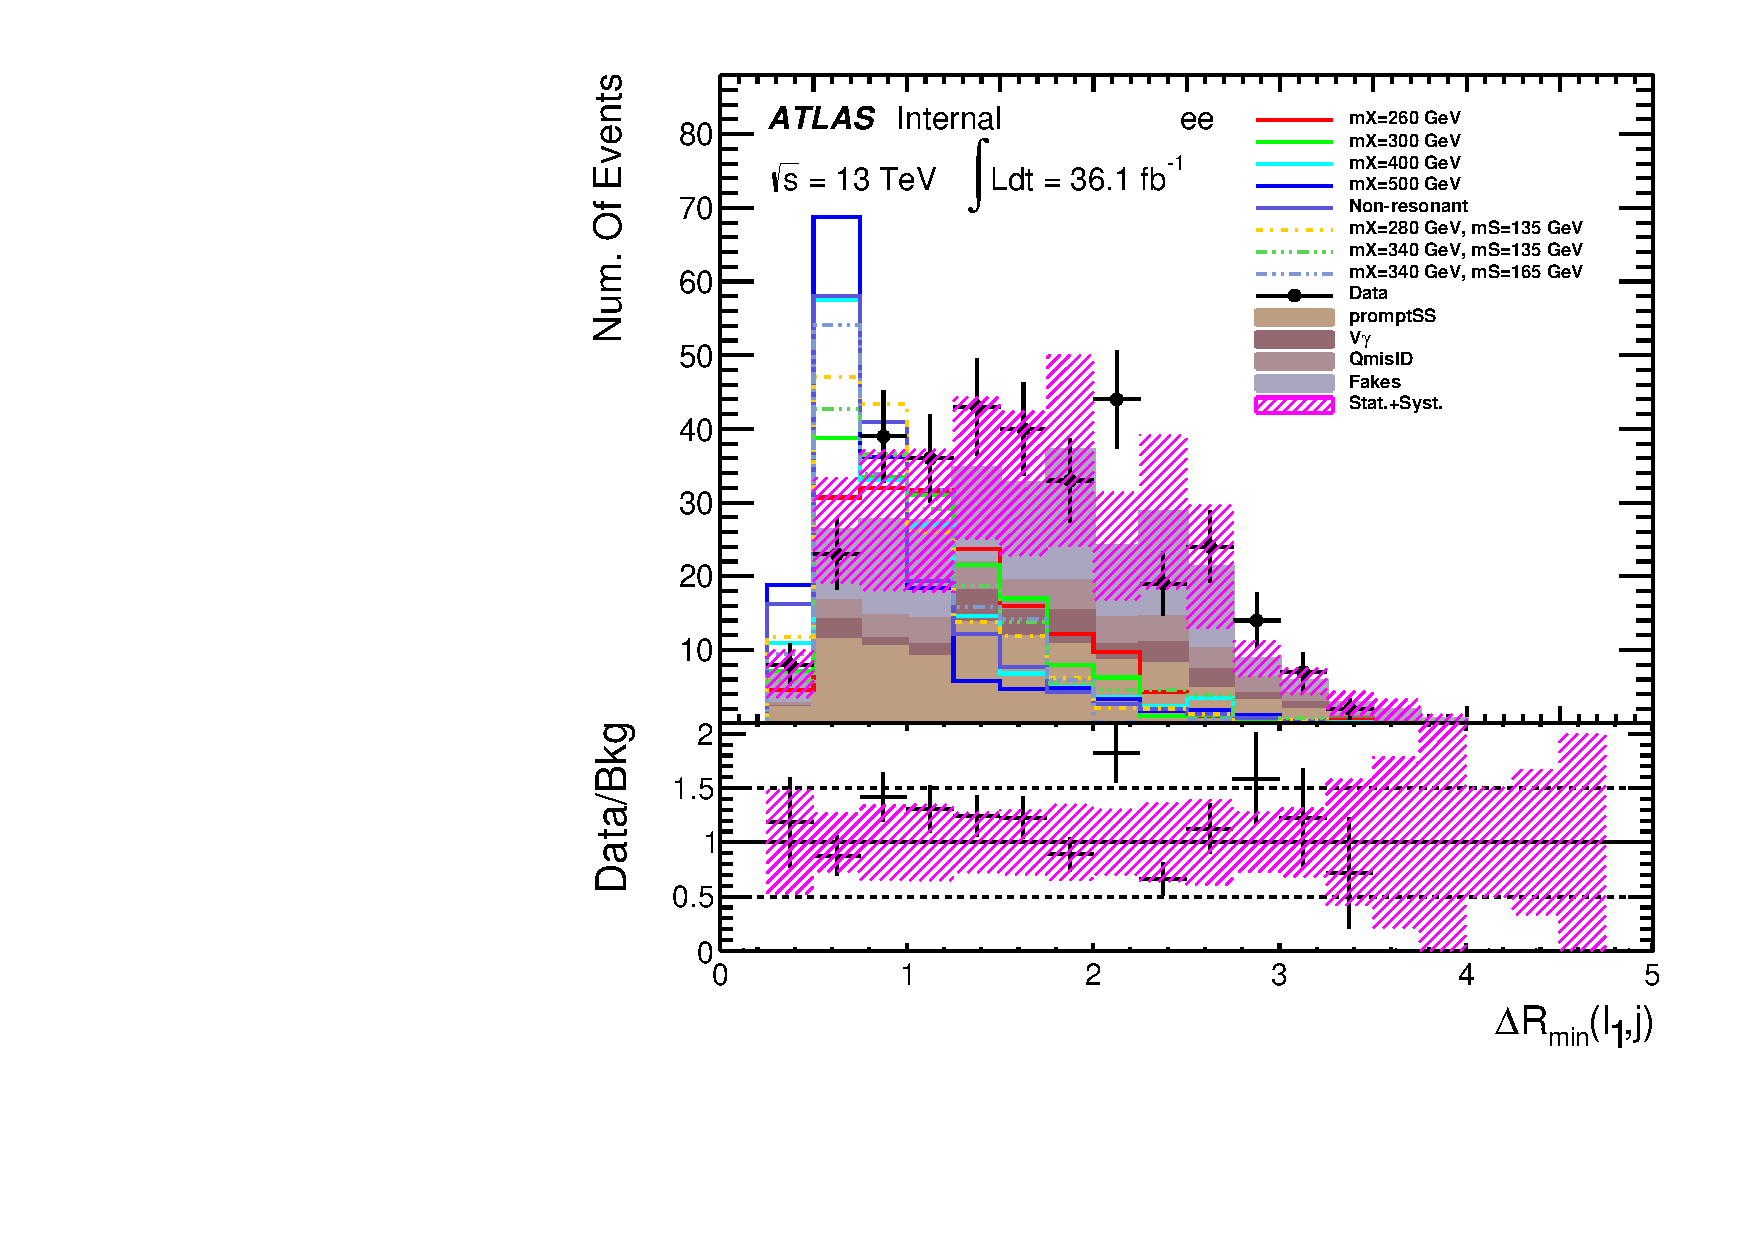
\includegraphics[width=1.0\textwidth]{fig/dataMC_high_Njet_CR/mindR_l1j_ee.pdf}\label{fig:dataMC_high_Njet_CR:mindRl1j_ee.pdf}
 \end{minipage}
 \begin{minipage}[t]{0.33\linewidth}
 \centering
 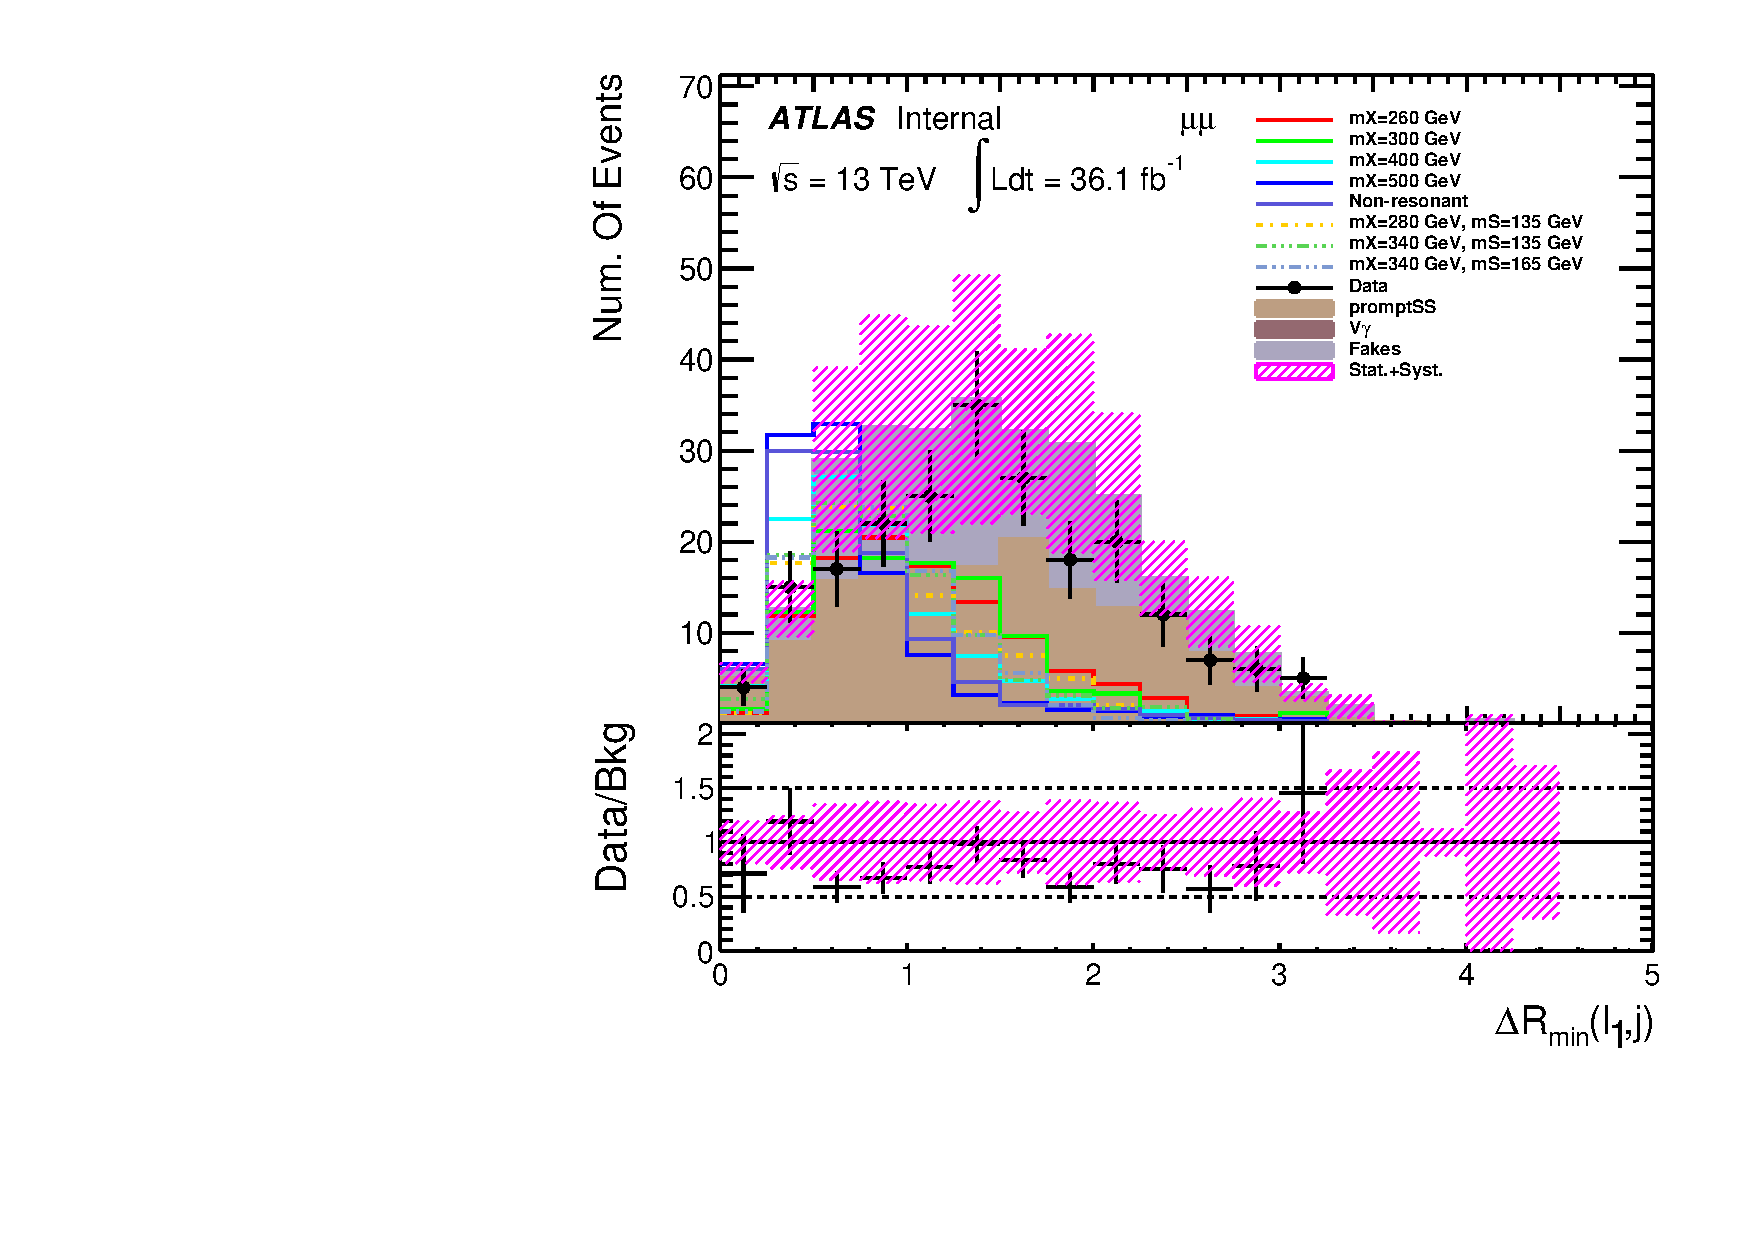
\includegraphics[width=1.0\textwidth]{fig/dataMC_high_Njet_CR/mindR_l1j_mumu.pdf}\label{fig:dataMC_high_Njet_CR:mindRl1j_mumu.pdf}
 \end{minipage}
  \begin{minipage}[t]{0.33\linewidth}
 \centering
 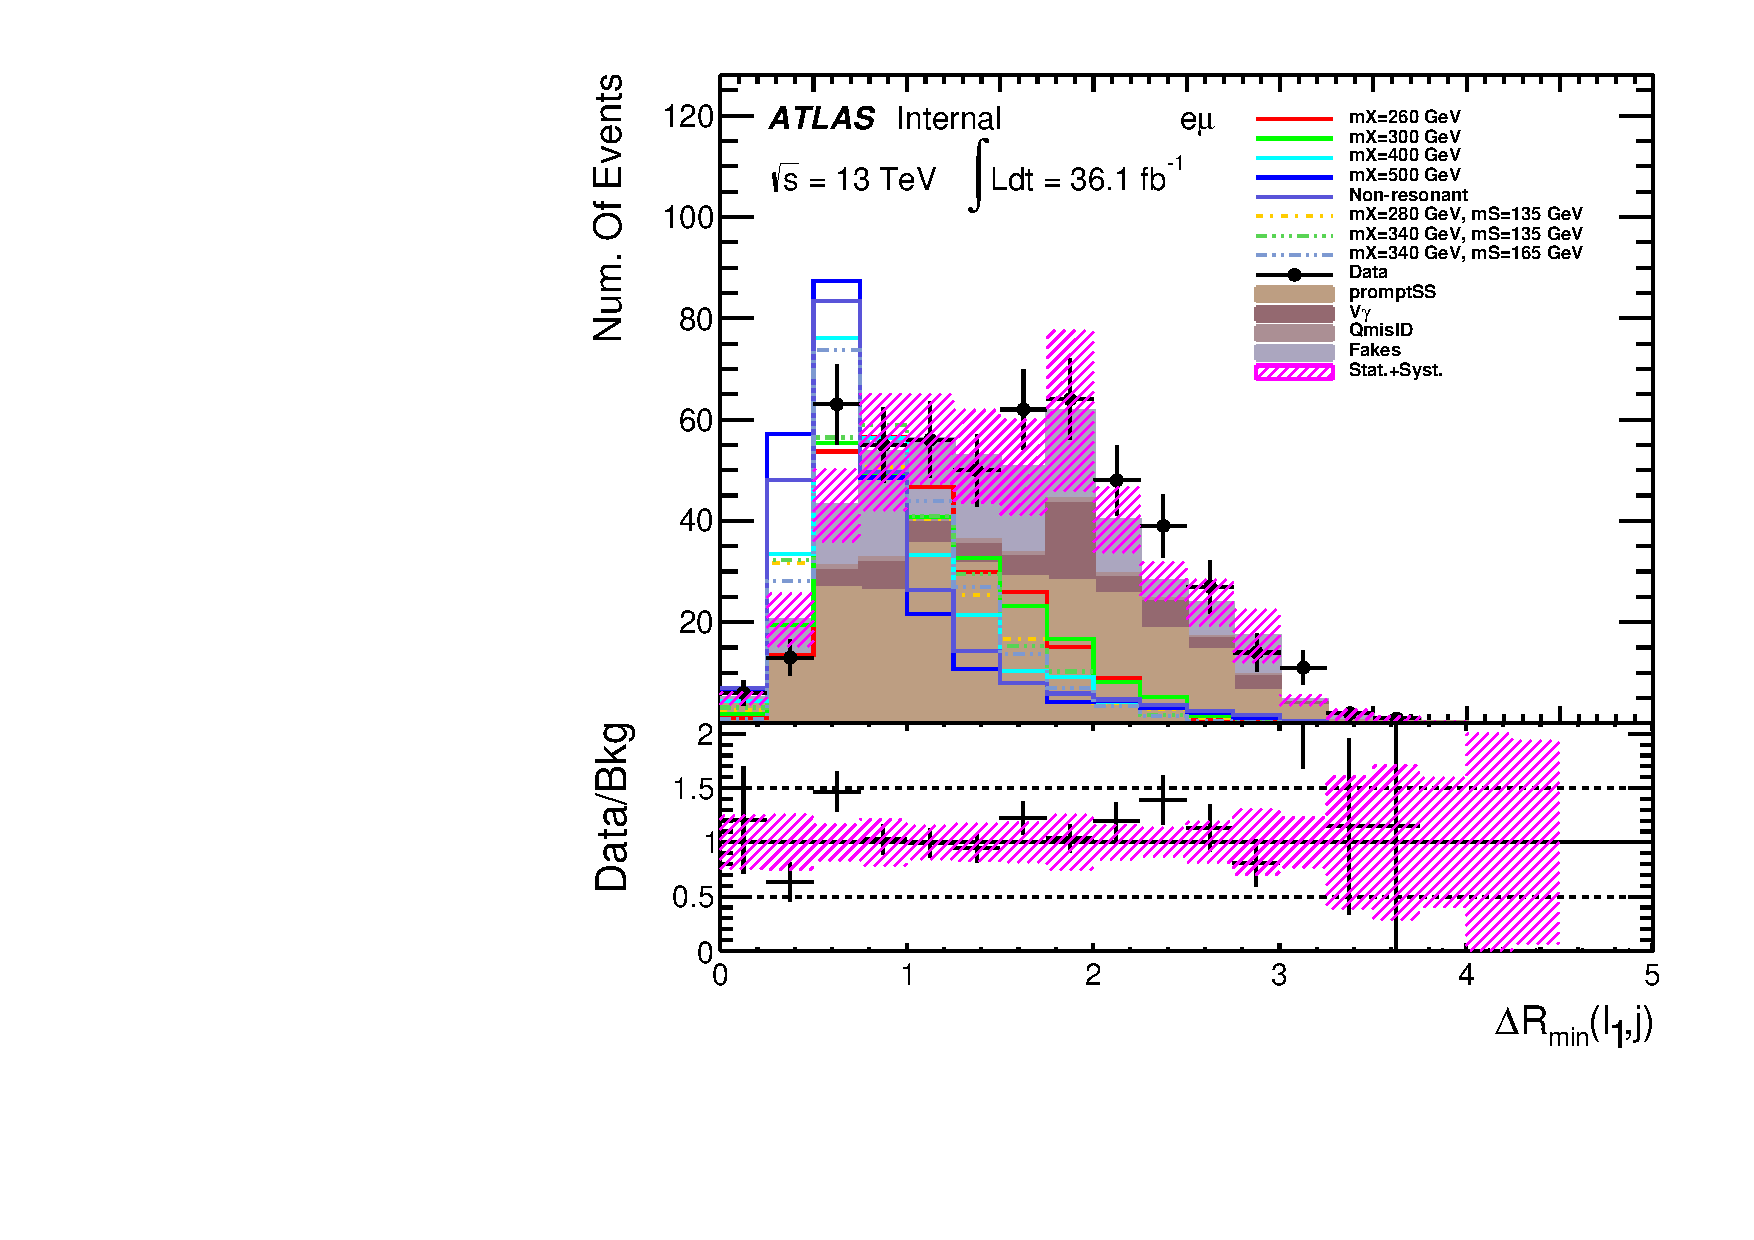
\includegraphics[width=1.0\textwidth]{fig/dataMC_high_Njet_CR/mindR_l1j_emu.pdf}\label{fig:dataMC_high_Njet_CR:mindRl1j_emu.pdf}
 \end{minipage}
\begin{minipage}[t]{0.33\linewidth}
 \centering
 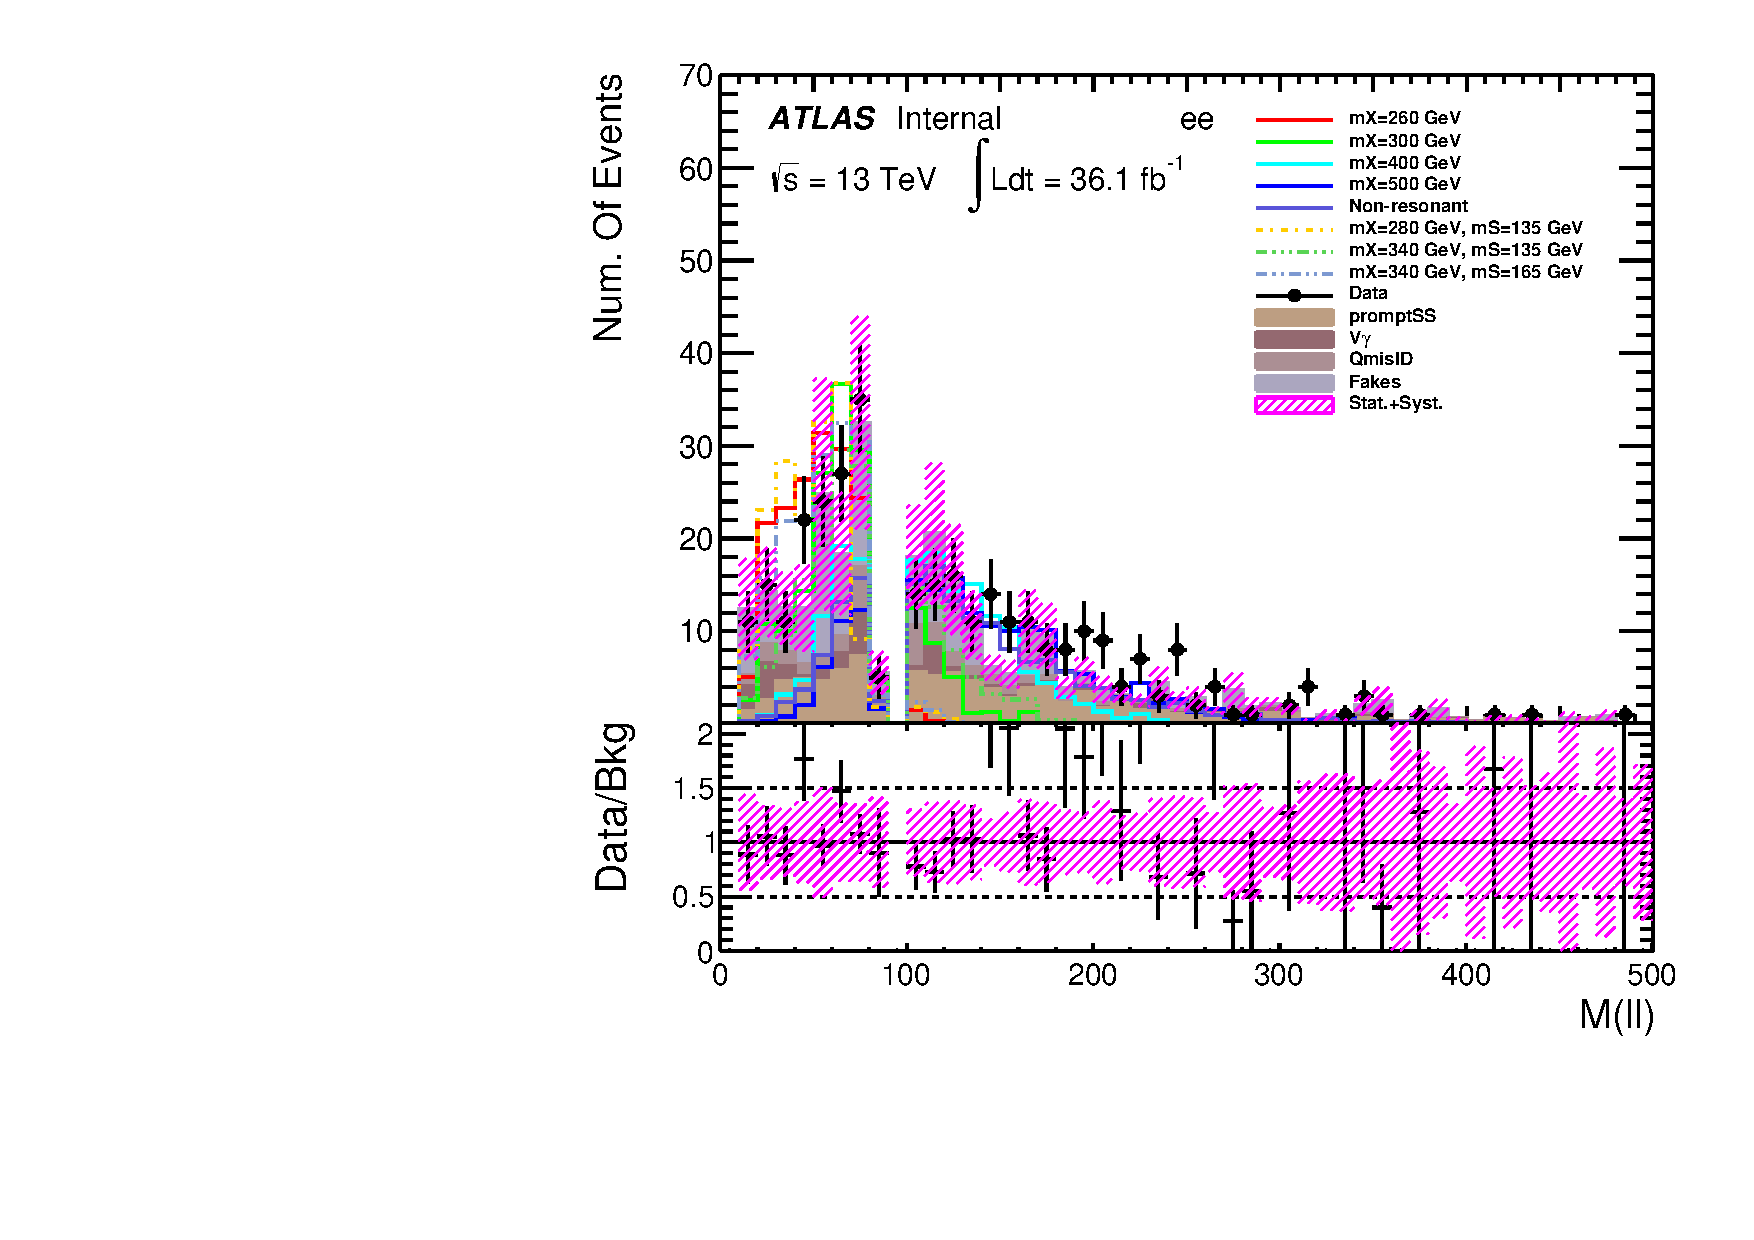
\includegraphics[width=1.0\textwidth]{fig/dataMC_high_Njet_CR/m_ll_ee.pdf}
 \label{fig:dataMC_high_Njet_CR:m_ll_ee.pdf}
 \end{minipage}
 \begin{minipage}[t]{0.33\linewidth}
 \centering
 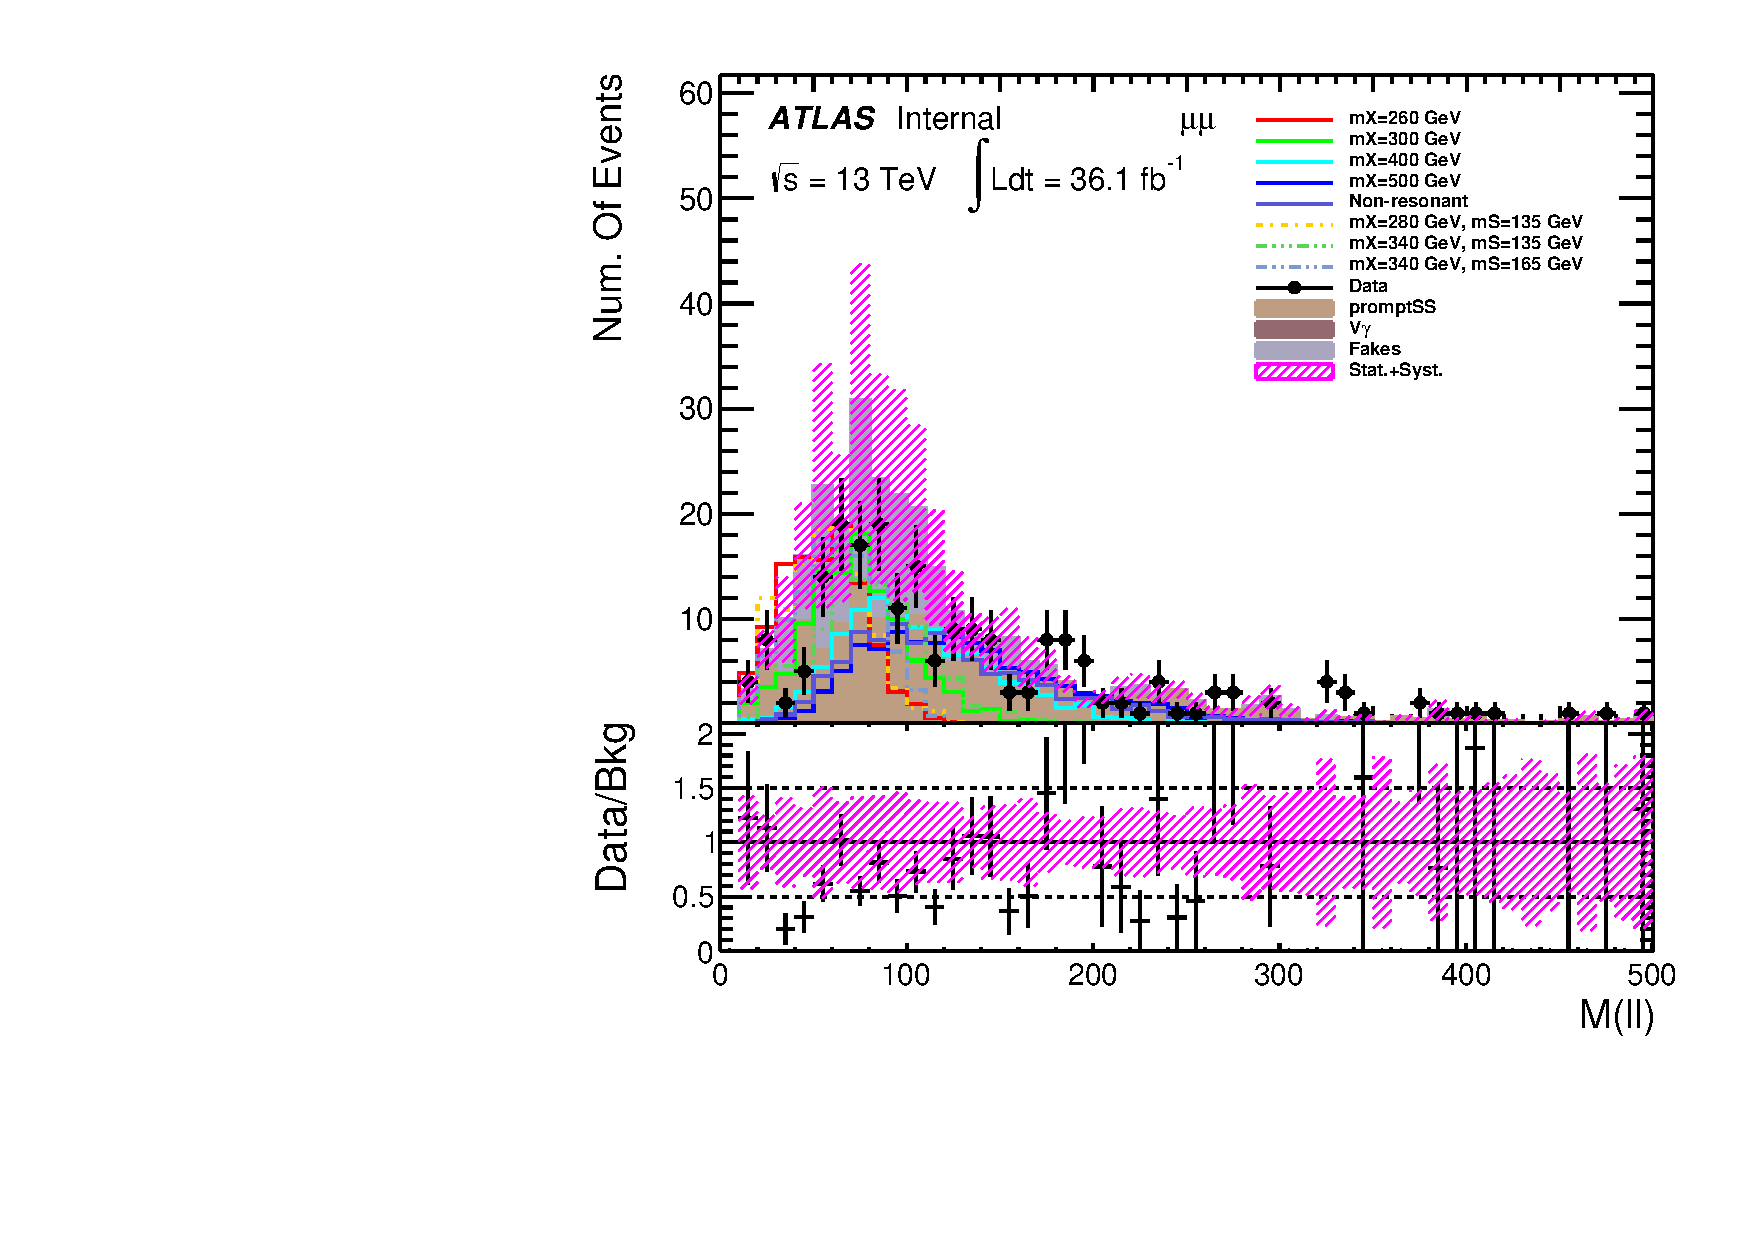
\includegraphics[width=1.0\textwidth]{fig/dataMC_high_Njet_CR/m_ll_mumu.pdf}
 \label{fig:dataMC_high_Njet_CR:m_ll_mumu.pdf}
 \end{minipage}
 \begin{minipage}[t]{0.33\linewidth}
 \centering
 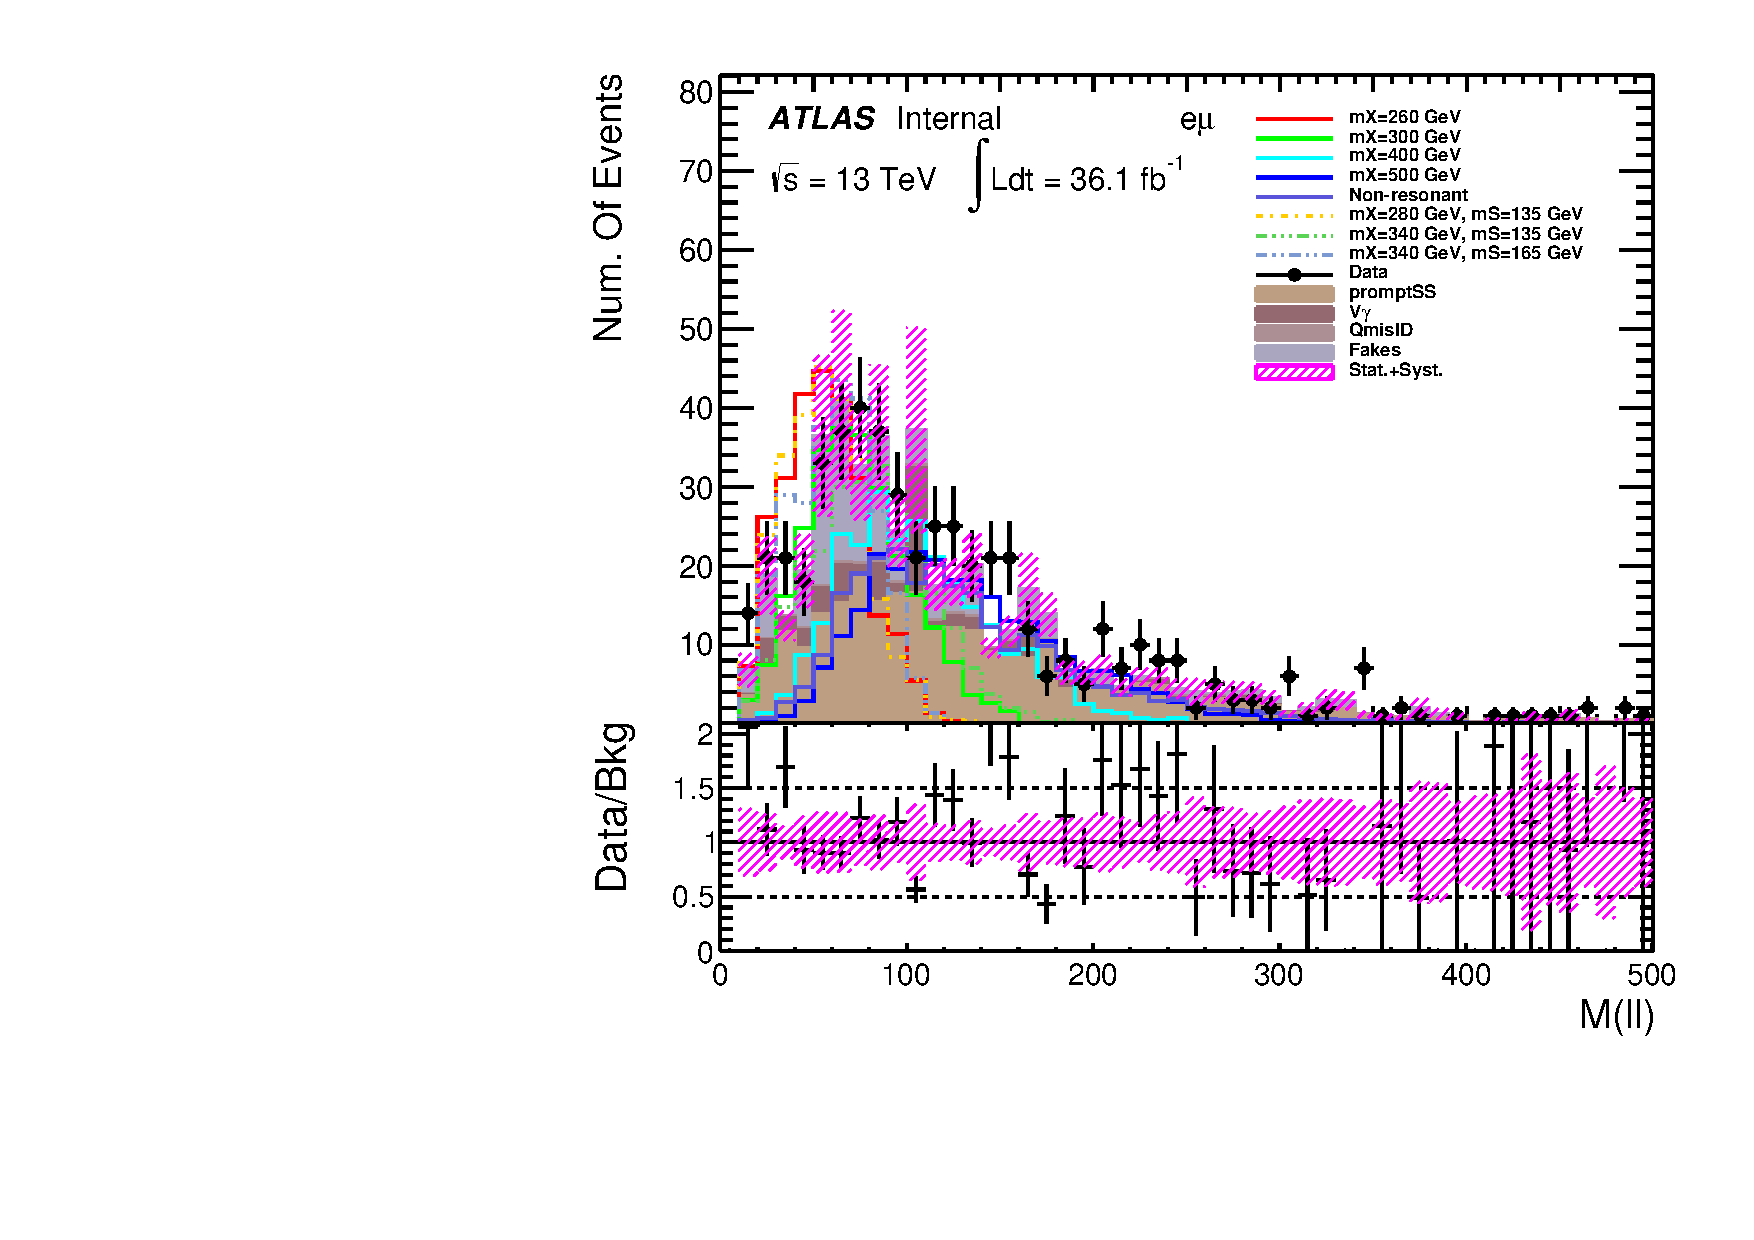
\includegraphics[width=1.0\textwidth]{fig/dataMC_high_Njet_CR/m_ll_emu.pdf}
 \label{fig:dataMC_high_Njet_CR:m_ll_emu.pdf}
 \end{minipage}
\begin{minipage}[t]{0.33\linewidth}
 \centering
 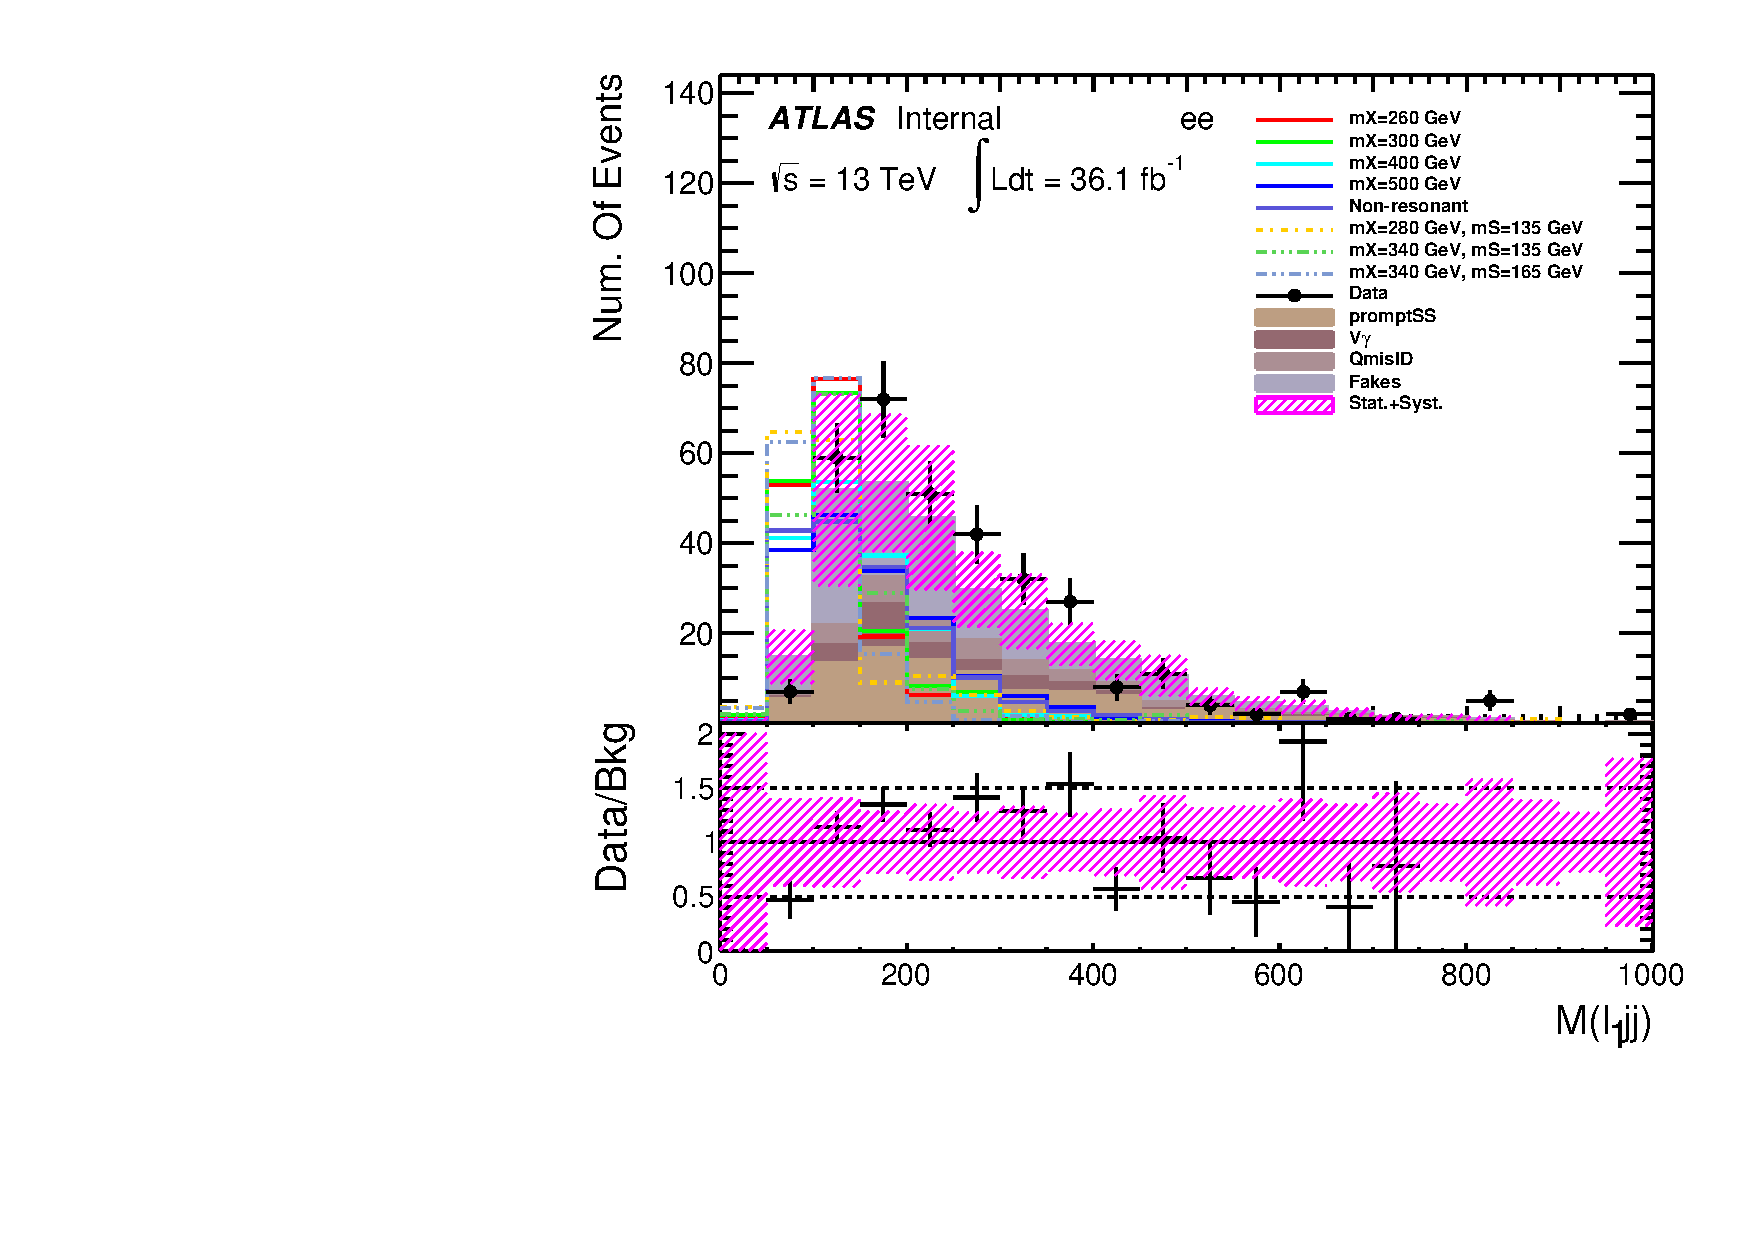
\includegraphics[width=1.0\textwidth]{fig/dataMC_high_Njet_CR/m_l1jj_ee.pdf}\label{fig:dataMC_high_Njet_CR:m_l1jj_ee.pdf}
 \end{minipage}
  \begin{minipage}[t]{0.33\linewidth}
 \centering
 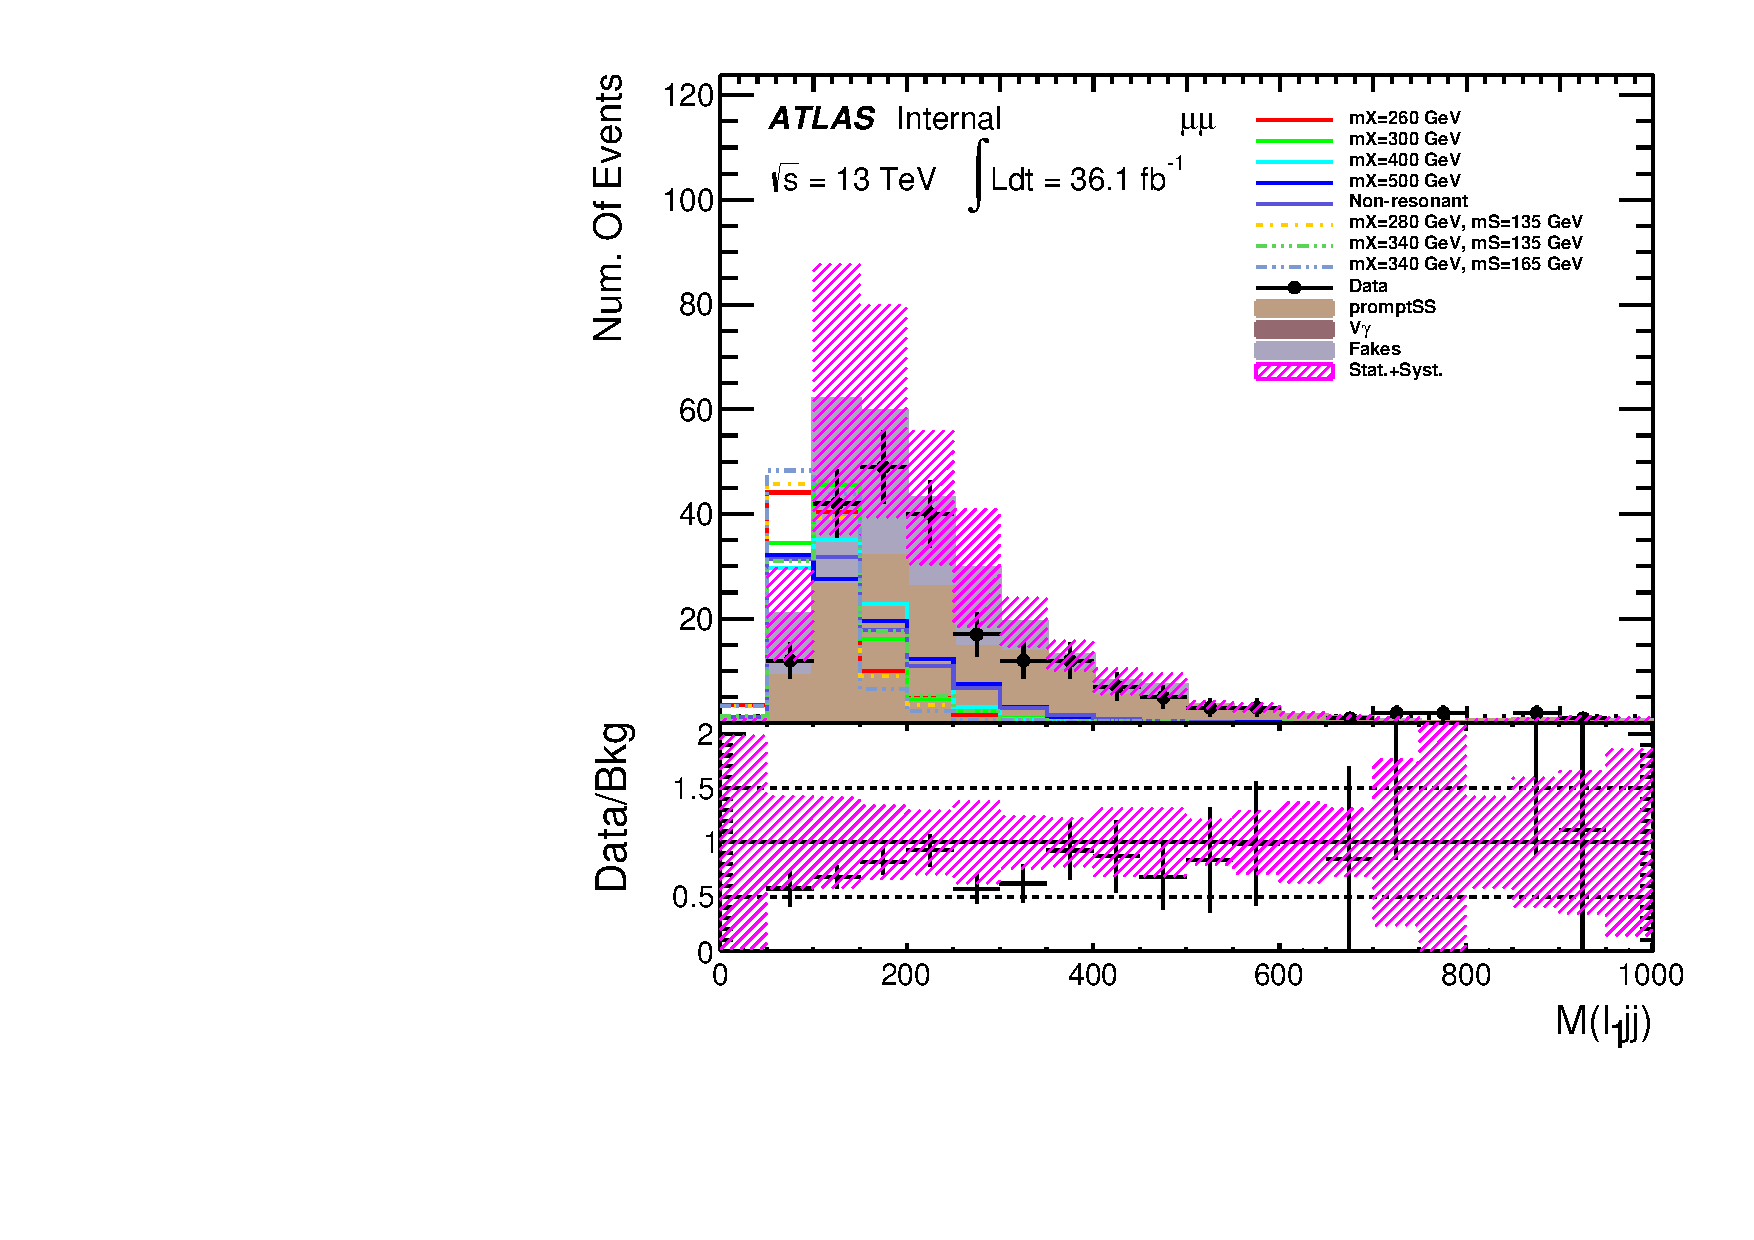
\includegraphics[width=1.0\textwidth]{fig/dataMC_high_Njet_CR/m_l1jj_mumu.pdf}\label{fig:dataMC_high_Njet_CR:m_l1jj_mumu.pdf}
 \end{minipage}
 \begin{minipage}[t]{0.33\linewidth}
 \centering
 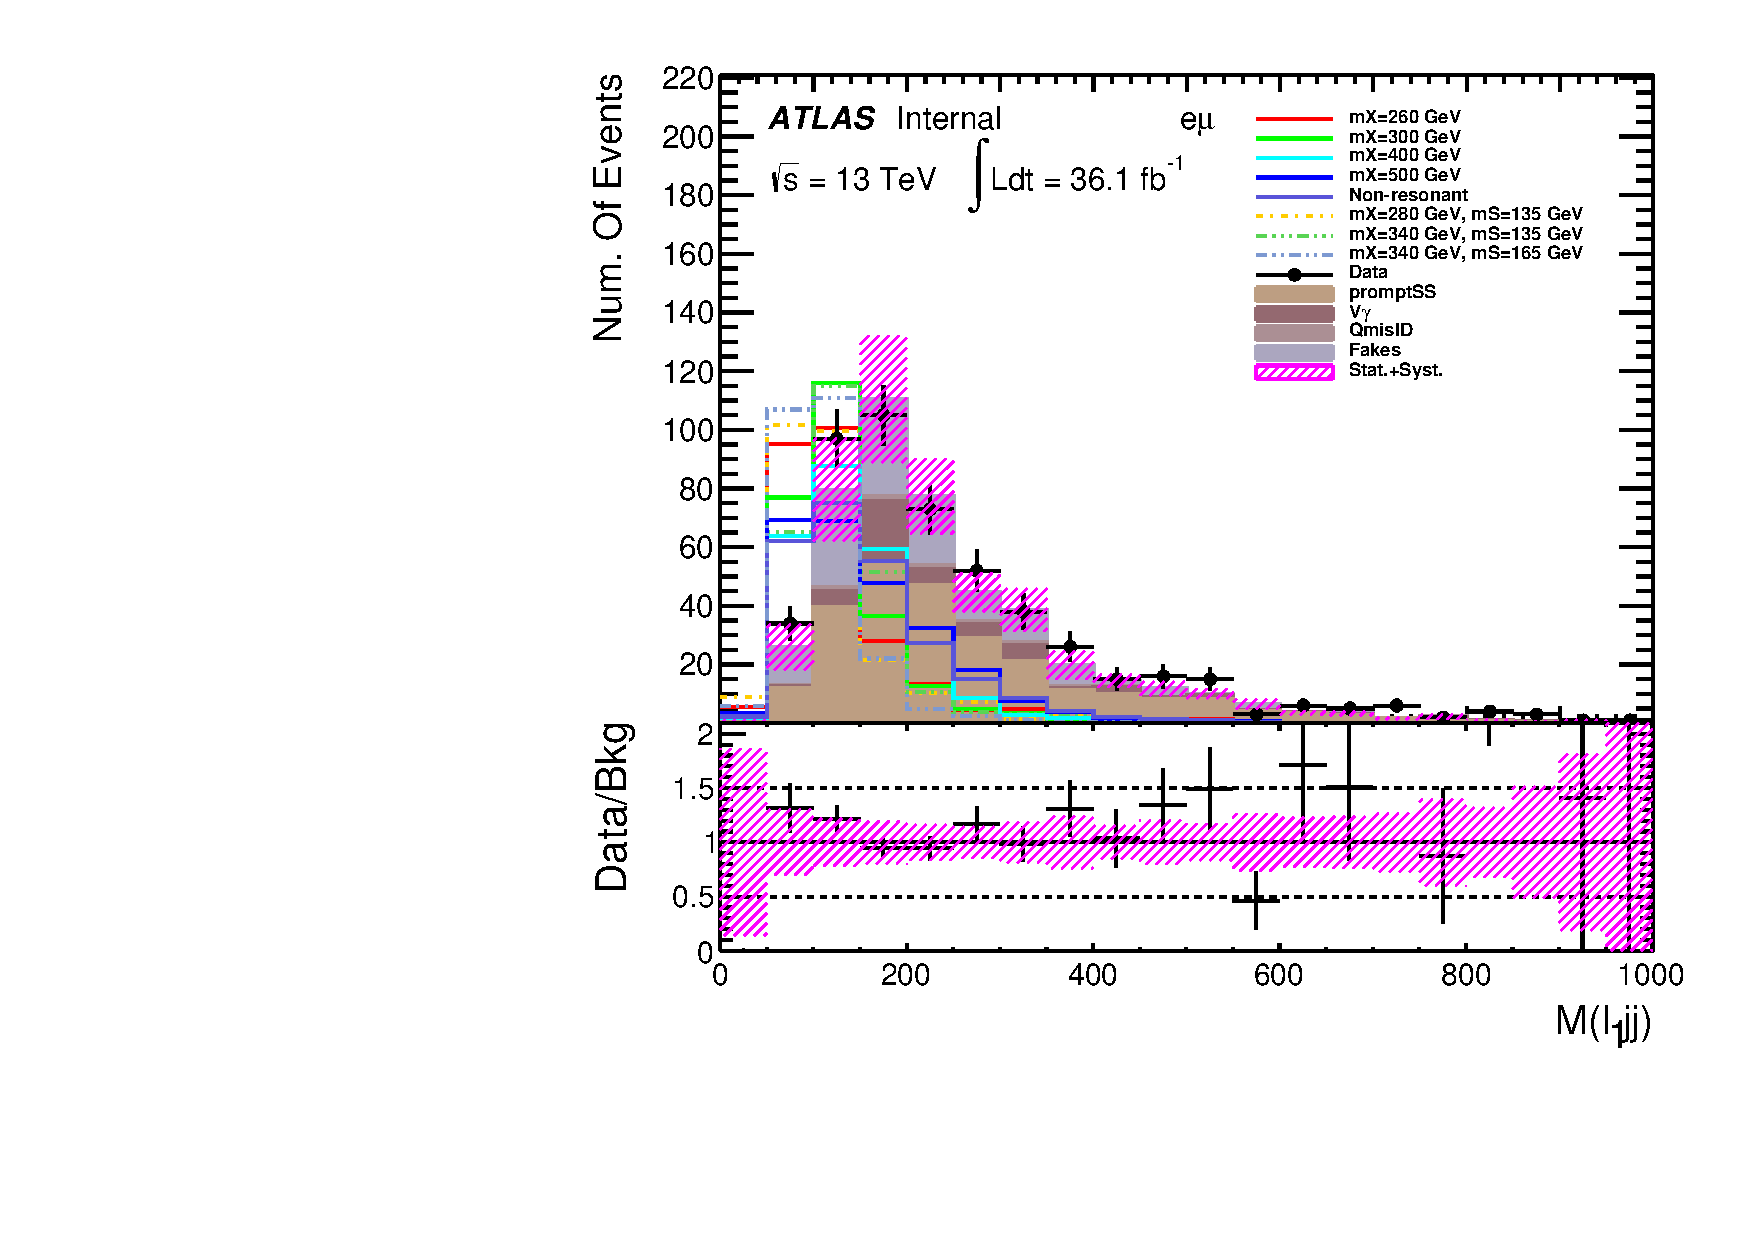
\includegraphics[width=1.0\textwidth]{fig/dataMC_high_Njet_CR/m_l1jj_emu.pdf}\label{fig:dataMC_high_Njet_CR:m_l1jj_emu.pdf}
 \end{minipage}
 \caption{The distributions of kinematic variables that are used to form optimization selections at pre-selection level, corresponding to $N_{\text{jet}}\geq3$. Left: $ee$, middle: $\mu\mu$, right: $e\mu$. PromptSS and $V+\gamma$ are normalized to the luminosity of 36.1 fb$^{-1}$.}
\label{fig:SigOpt_high_kine}
\end{figure}
\begin{figure}[h]
\begin{center}
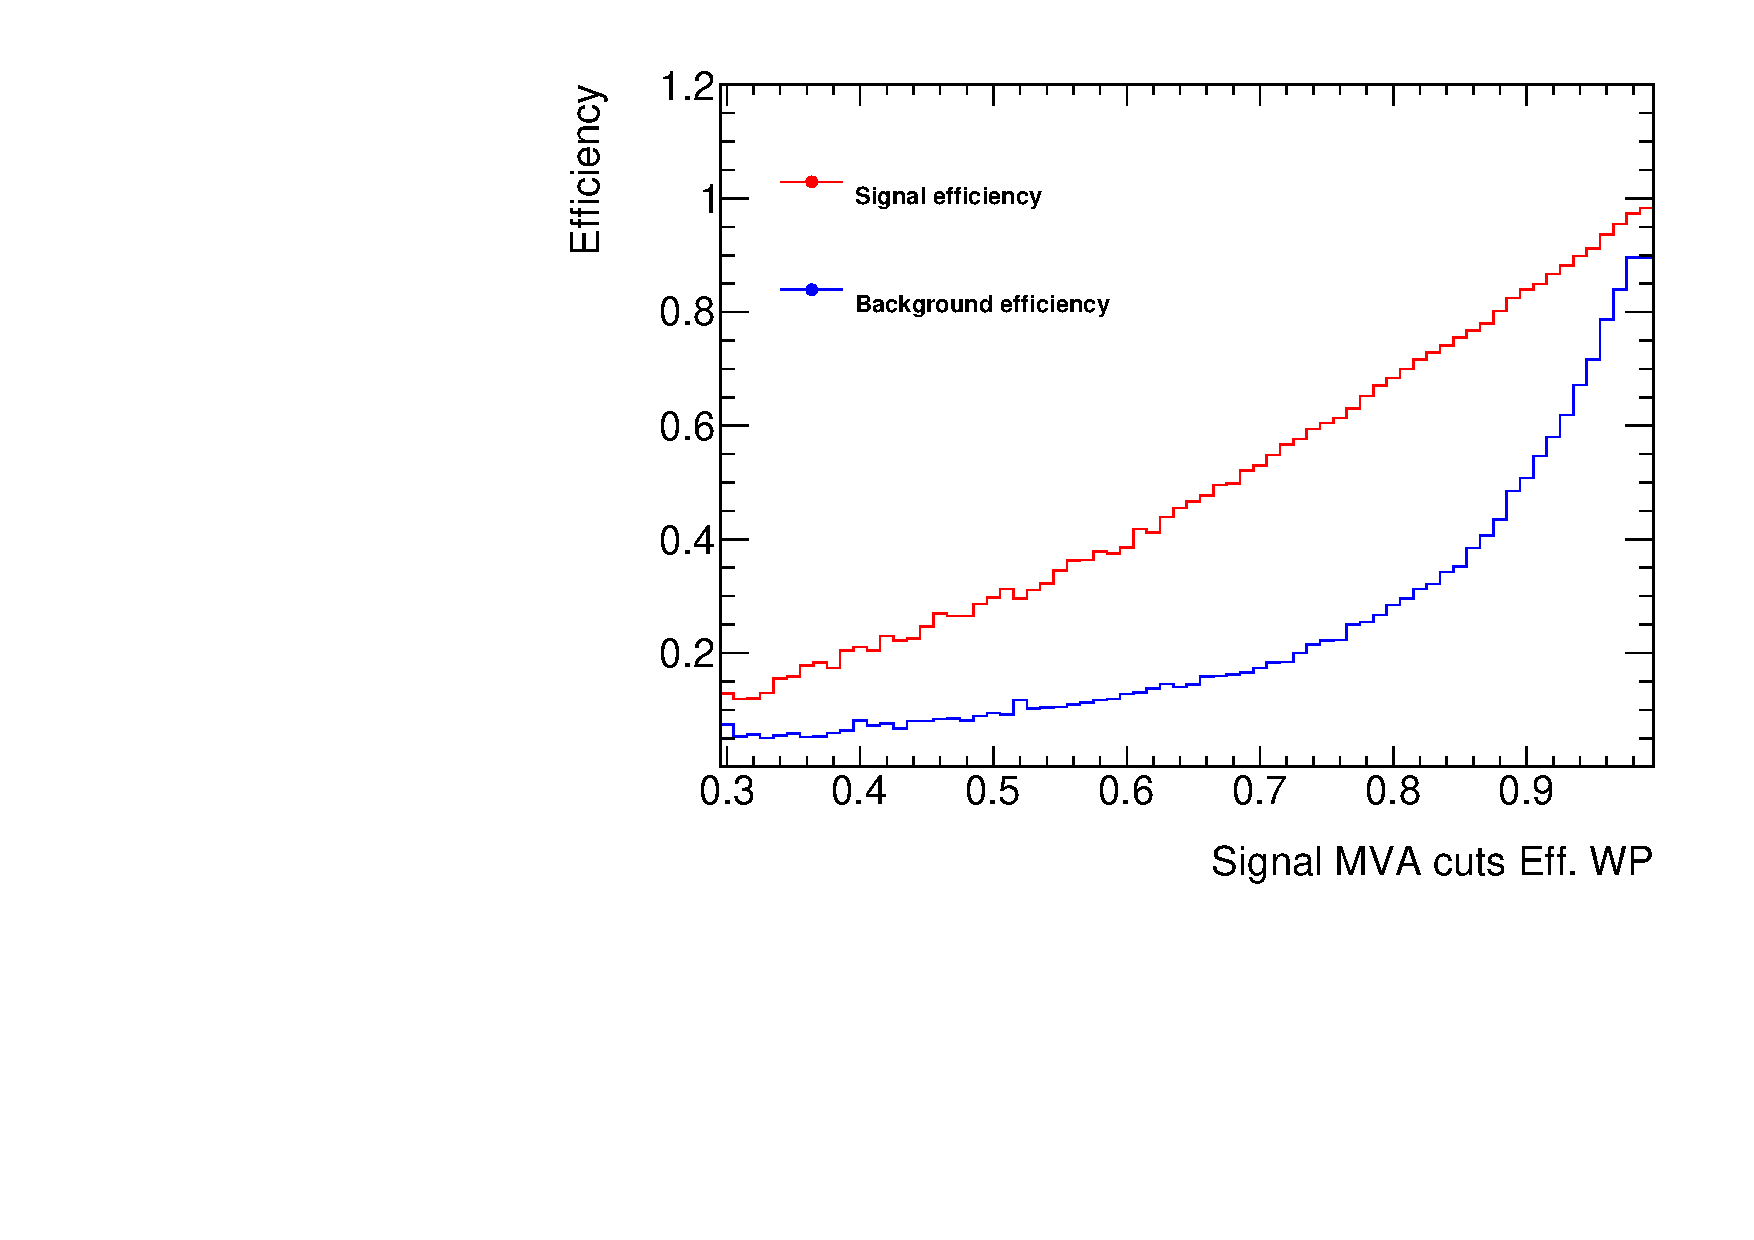
\includegraphics[width = 0.4\textwidth]{fig/SigOpt/nonres/Efficiency_mumu.pdf}
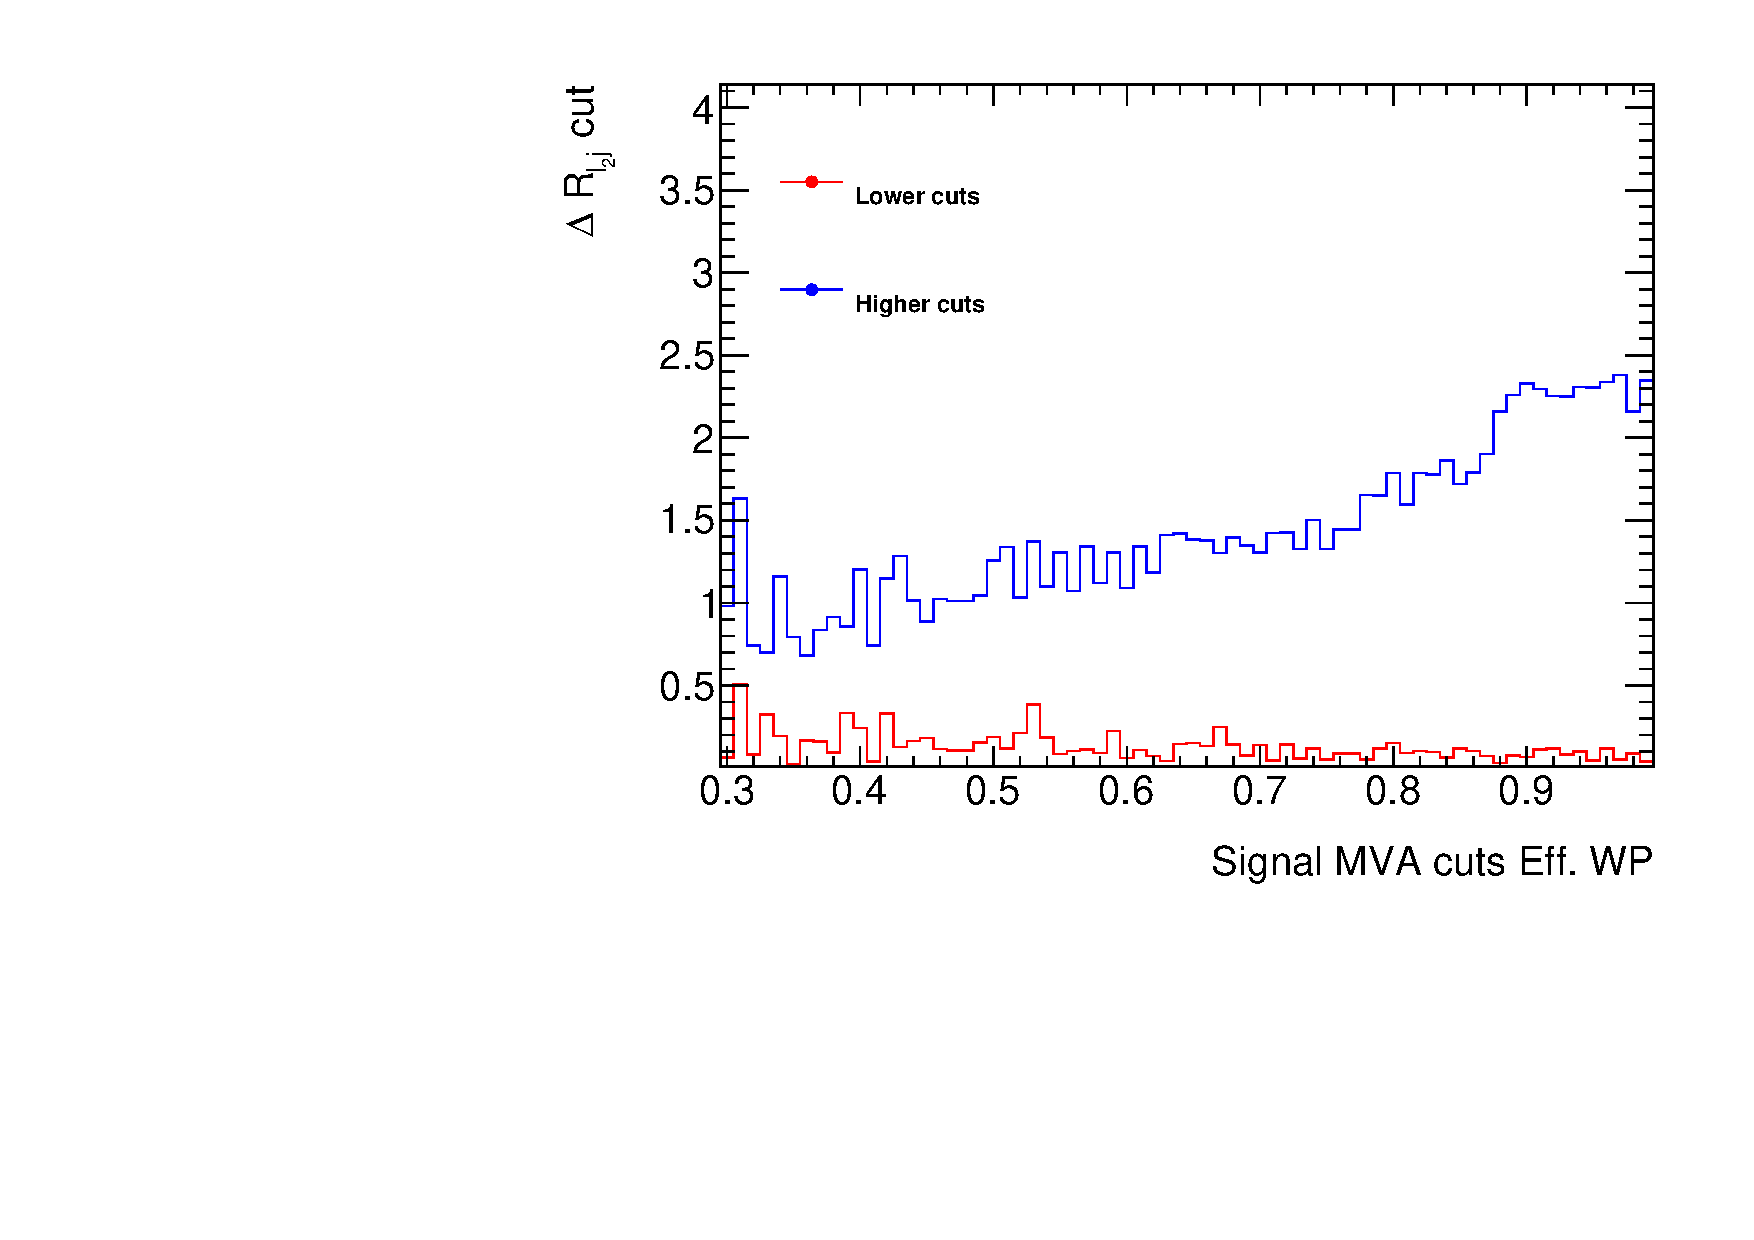
\includegraphics[width = 0.4\textwidth]{fig/SigOpt/nonres/mindR_l2j_mumu.pdf}
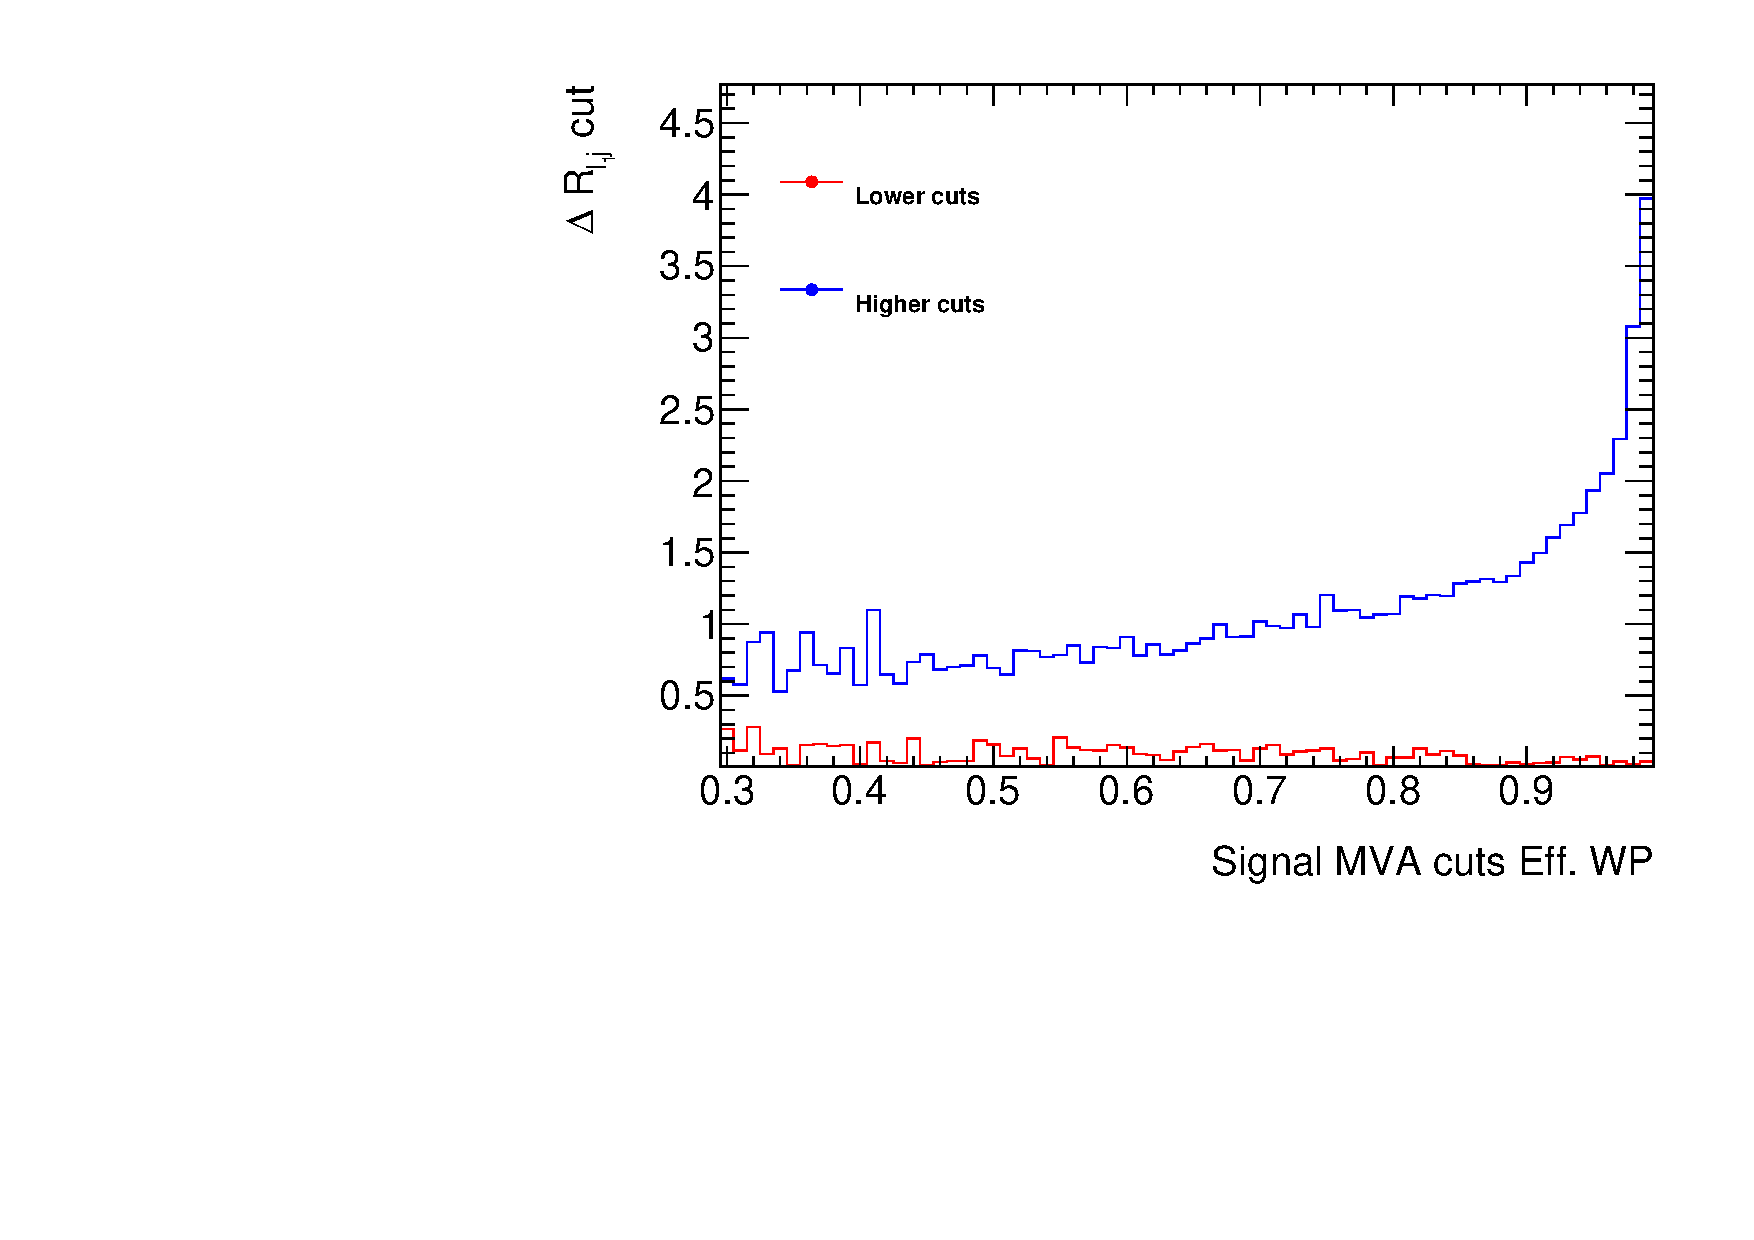
\includegraphics[width = 0.4\textwidth]{fig/SigOpt/nonres/mindR_l1j_mumu.pdf}
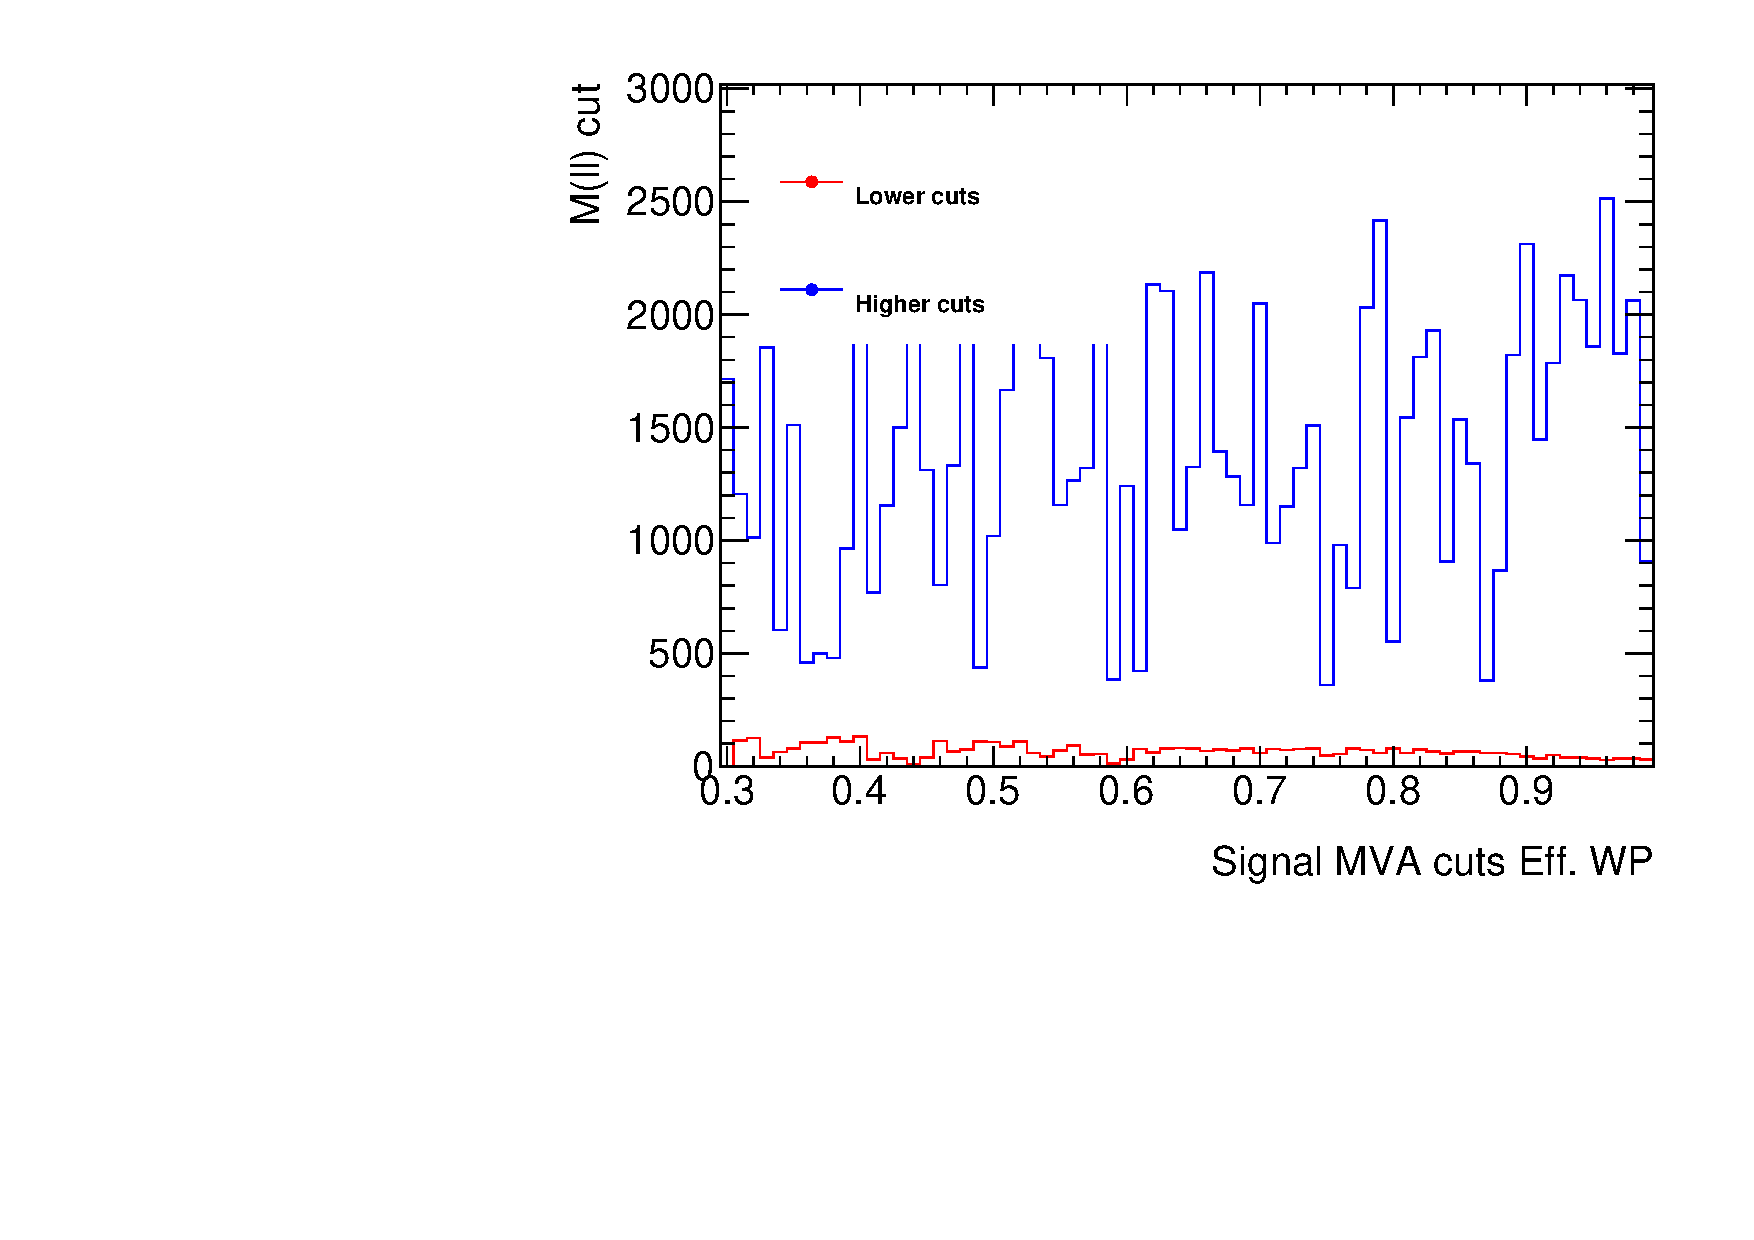
\includegraphics[width = 0.4\textwidth]{fig/SigOpt/nonres/m_ll_mumu.pdf}
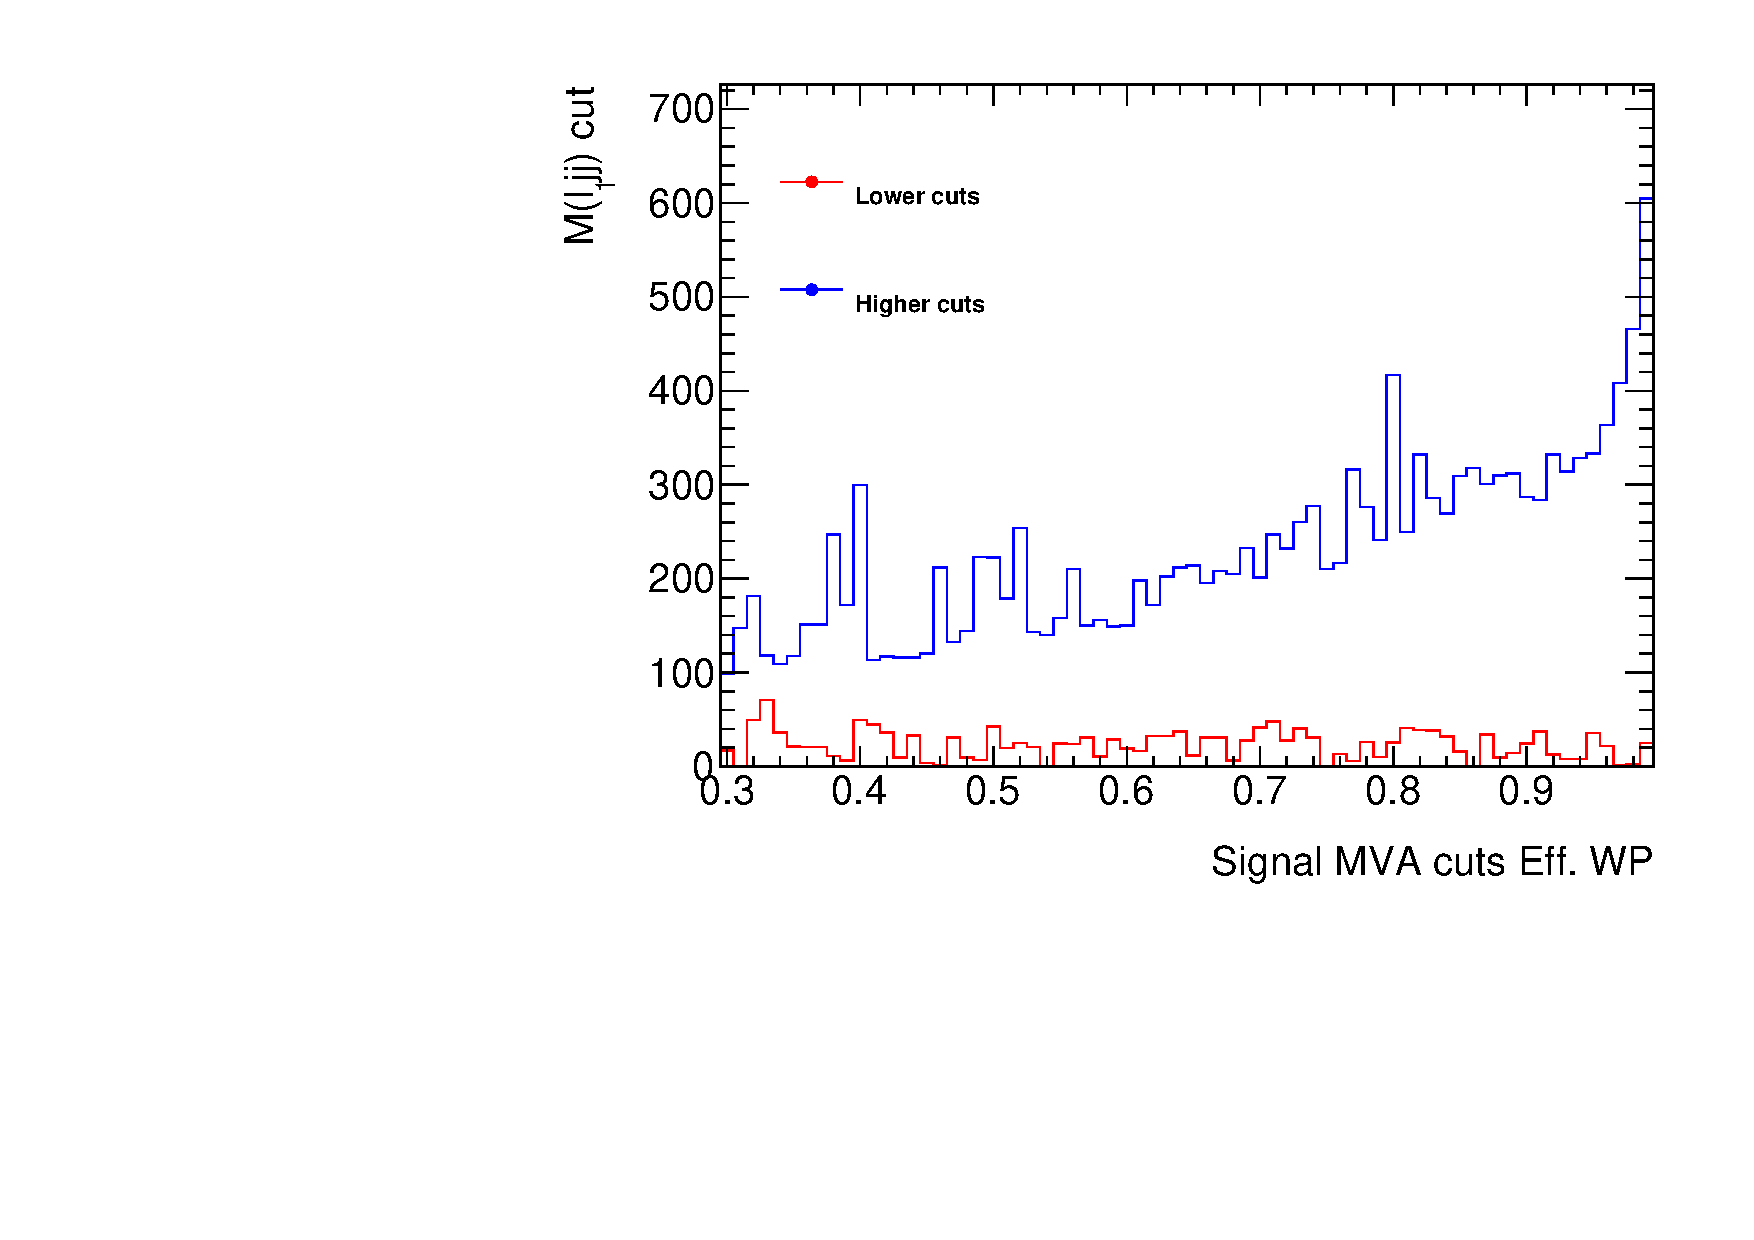
\includegraphics[width = 0.4\textwidth]{fig/SigOpt/nonres/m_l1jj_mumu.pdf}
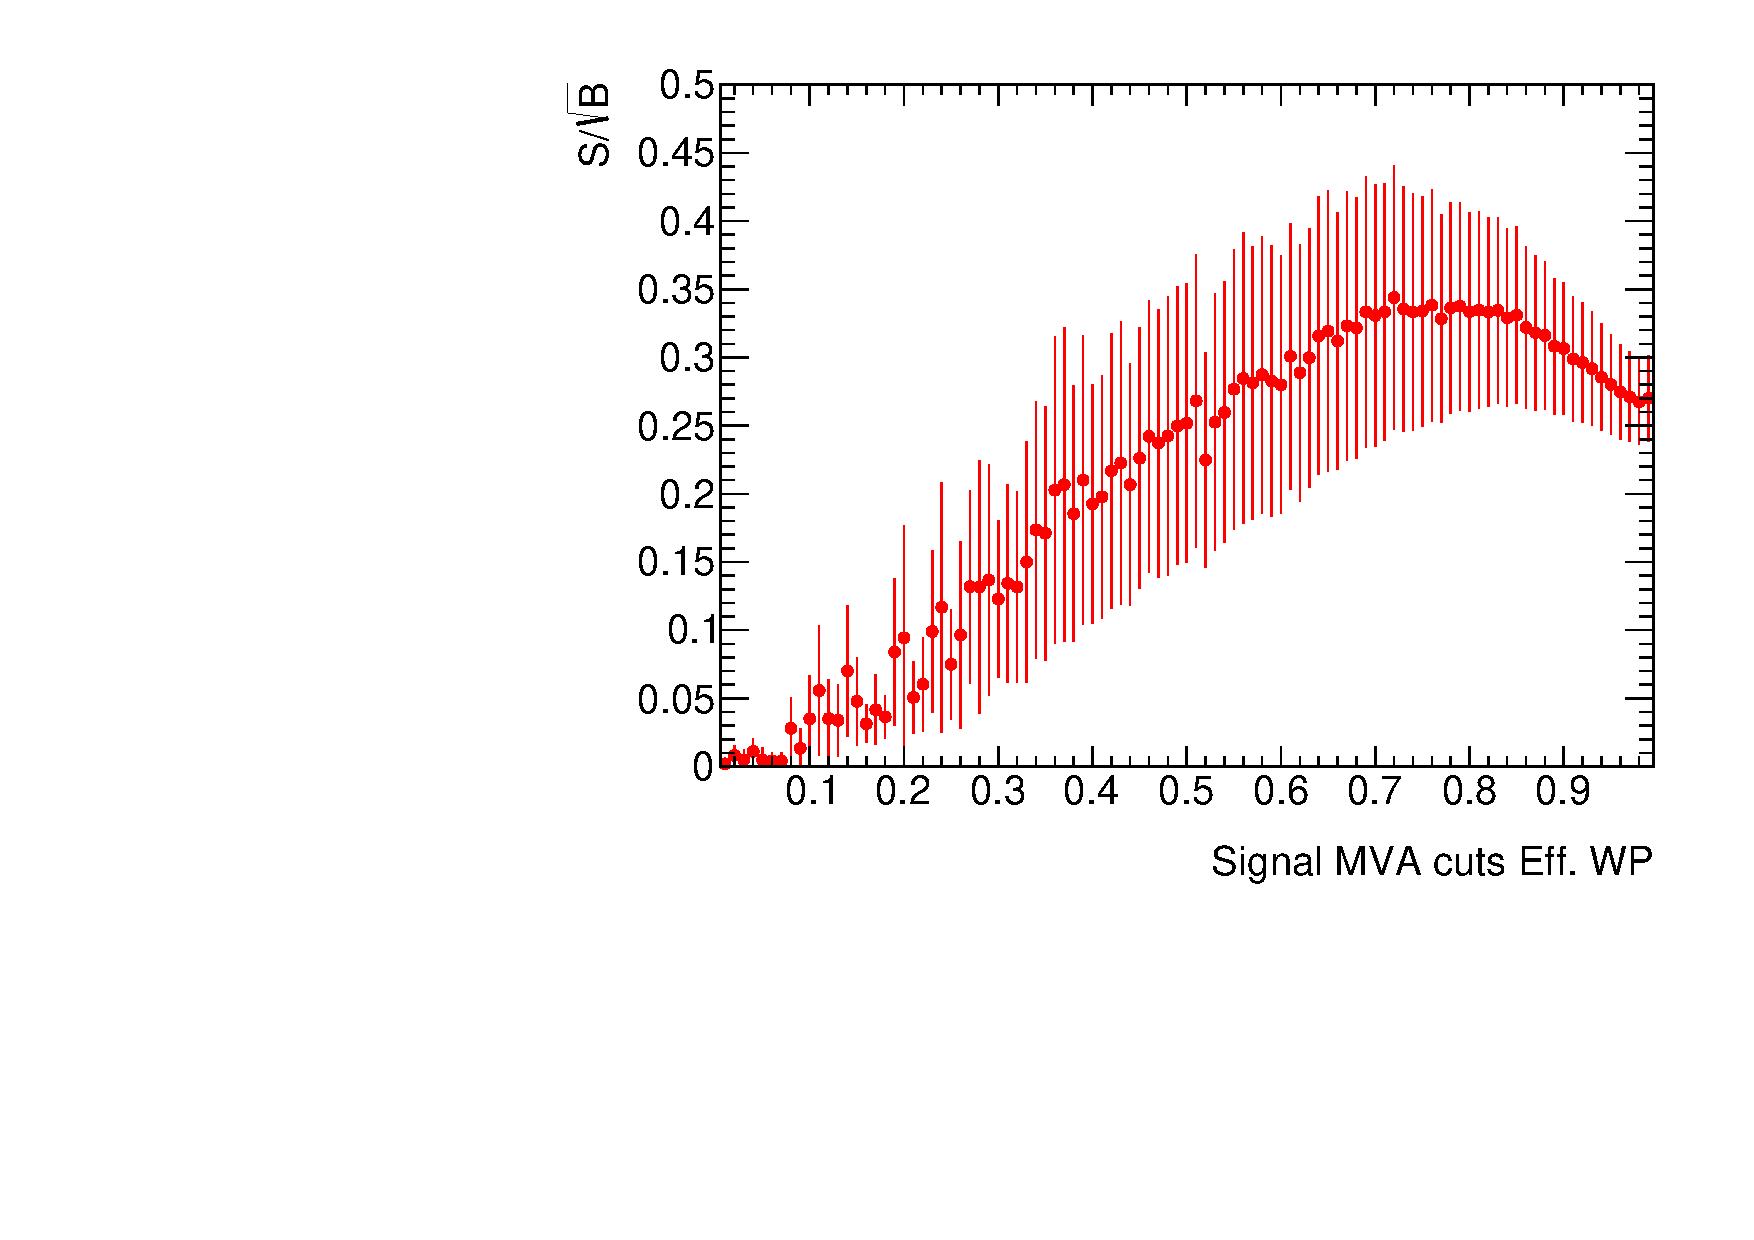
\includegraphics[width = 0.4\textwidth]{fig/SigOpt/nonres/SOverRootB_mumu.pdf}
\caption{The significance scan as a function of efficiency for $\mu\mu$ in non-resonant signal search. Statistical uncertainties on the background and the signal are considered. The 0.72 working point is chosen for $\mu\mu$ channel in the non-resonant signal optimizations.}
\label{fig:nonres:SigOpt_mumu}
\end{center}
\end{figure}

\begin{table}[h]
\begin{center}
\begin{tabular}{c|c|c|c|c|c}
\hline
\hline
  &Channel &$\Delta R_{min}(\ell_{1}, j)$ &$M(ll)$  &$M_{\ell_{1}jj}$ &$M(all)$\\
\hline
\multirow{3}{2.0cm}{$m_X$=260 GeV} &$ee$  &0.35, 1.85
&$<$100
&$<$145
&$<$1100  \\
&$\mu\mu$
&0.25, 2.10
&$<$80
&$<$115
&$<$700 \\
&$e\mu$
&0.25, 1.80
&$<$85
&$<$135
&$<$650\\
\hline
\multirow{3}{2.0cm}{$m_X$=300 GeV} &$ee$
&0.35, 1.75
&$<$120
&$<$160
&$<$1400 \\
&$\mu\mu$
&0.20, 1.75
&$<$115
&$<$185
&$<$1000 \\
&$e\mu$
&0.20, 1.80
&$<$135
&$<$160
&$<$800 \\
\hline
\hline
\end{tabular}
\end{center}
\caption{Summary of optimization selections for the search of $X \rightarrow hh$ ($m_{X}$=260, 300 GeV). All mass cuts are in GeV.}
\label{optimization_cuts_lowmass}
\end{table}

\begin{table}[h]
\begin{center}
\begin{tabular}{c|c|c|c|c|c}
\hline
\hline
  &Channel &$\Delta R_{min}(\ell_{2}, j)$ &$\Delta R_{min}(\ell_{1}, j)$ &$M(ll)$  &$M_{\ell_{1}jj}$ \\
\hline
\multirow{3}{2.0cm}{$m_X$=400 GeV} &$ee$
&0.35, 1.50
&0.30, 1.25
&45, 235
&40, 285 \\
&$\mu\mu$
&0.20, 1.20
&0.20, 1.20
&40, 215
&30, 260 \\
&$e\mu$
&0.20, 1.50
&0.20, 1.05
&35, 195
&30, 235 \\
\hline
\multirow{3}{2.0cm}{$m_X$=500 GeV} &$ee$
&0.20, 1.15
&0.20, 1.15
&100, 270
&40, 285 \\
&$\mu\mu$
&0.20, 1.05
&0.20, 0.75
&60, 250
&30, 310 \\
&$e\mu$
&0.20, 1.00
&0.20, 0.80
&75, 250
&35, 350 \\
\hline
\multirow{3}{2.0cm}{Non-resonant} & $ee$
&0.20, 1.40
&0.20, 1.15
&55, 270
&40, 285 \\
&$\mu\mu$
&0.20, 1.05
&0.20, 0.75
&60, 250
&30, 310 \\
&$e\mu$
&0.20, 1.15
&0.20, 0.80
&75, 250
&35, 350 \\
\hline
\hline
\end{tabular}
\end{center}
\caption{Summary of optimization selections for the search of $X \rightarrow hh$($m_{X}$=400, 500 GeV and non-resonant). All mass cuts are in GeV.}
\label{optimization_cuts_highmass}
\end{table}
 
\section{信号效率}


\section{优化结果}
